
\documentclass[preprint,12pt,sort&compress]{elsarticle}

%% Use the option review to obtain double line spacing
%% \documentclass[preprint,review,12pt]{elsarticle}

%% Use the options 1p,twocolumn; 3p; 3p,twocolumn; 5p; or 5p,twocolumn
%% for a journal layout:
%% \documentclass[final,1p,times]{elsarticle}
%% \documentclass[final,1p,times,twocolumn]{elsarticle}
%% \documentclass[final,3p,times]{elsarticle}
%% \documentclass[final,3p,times,twocolumn]{elsarticle}
%% \documentclass[final,5p,times]{elsarticle}
%% \documentclass[final,5p,times,twocolumn]{elsarticle}


%% The graphicx package provides the includegraphics command.
\usepackage{graphicx}
%% The amssymb package provides various useful mathematical symbols
\usepackage{amssymb}
%% The amsthm package provides extended theorem environments
\usepackage{amsthm}
\usepackage{amsmath}
\usepackage{breqn}


%% The lineno packages adds line numbers. Start line numbering with
%% \begin{linenumbers}, end it with \end{linenumbers}. Or switch it on
%% for the whole article with \linenumbers after \end{frontmatter}.
\usepackage{lineno}
\usepackage{url}
\usepackage{color}

\usepackage{changepage}
\usepackage{comment}

\usepackage{color}

\usepackage[colorinlistoftodos]{todonotes}
\definecolor{correction}{RGB}{0,0,0}
\definecolor{cut}{RGB}{255,131,0}

\definecolor{reviewer1}{RGB}{184, 111, 60}
\definecolor{reviewer2}{RGB}{160, 92, 123}

\newcommand{\rone}[1]{\textcolor{reviewer1}{#1}}
\newcommand{\rtwo}[1]{\textcolor{reviewer2}{#1}}

%% natbib.sty is loaded by default. However, natbib options can be
%% provided with \biboptions{...} command. Following options are
%% valid:

%%   round  -  round parentheses are used (default)
%%   square -  square brackets are used   [option]
%%   curly  -  curly braces are used      {option}
%%   angle  -  angle brackets are used    <option>
%%   semicolon  -  multiple citations separated by semi-colon
%%   colon  - same as semicolon, an earlier confusion
%%   comma  -  separated by comma
%%   numbers-  selects numerical citations
%%   super  -  numerical citations as superscripts
%%   sort   -  sorts multiple citations according to order in ref. list
%%   sort&compress   -  like sort, but also compresses numerical citations
%%   compress - compresses without sorting
%%
%% \biboptions{comma,round}

% \biboptions{}

\newtheorem{definition}{Definition}[section]


\newcommand{\eat}[1]{}
\newcommand{\scream}[1]{{\bf * #1 *}{\typeout{#1}}}

\journal{Journal Name}

\begin{document}

\begin{frontmatter}



%% Title, authors and addresses
\title{Credit Distribution in Relational Scientific Databases}

%% use the tnoteref command within \title for footnotes;
%% use the tnotetext command for the associated footnote;
%% use the fnref command within \author or \address for footnotes;
%% use the fntext command for the associated footnote;
%% use the corref command within \author for corresponding author footnotes;
%% use the cortext command for the associated footnote;
%% use the ead command for the email address,
%% and the form \ead[url] for the home page:
%%
%% \title{Title\tnoteref{label1}}
%% \tnotetext[label1]{}
%% \author{Name\corref{cor1}\fnref{label2}}
%% \ead{email address}
%% \ead[url]{home page}
%% \fntext[label2]{}
%% \cortext[cor1]{}
%% \address{Address\fnref{label3}}
%% \fntext[label3]{}


%% use optional labels to link authors explicitly to addresses:
%% \author[label1,label2]{<author name>}
%% \address[label1]{<address>}
%% \address[label2]{<address>}

\author[lab1]{Dennis Dosso}
\author[lab2]{Susan B. Davidson}
\author[lab1]{Gianmaria Silvello}
\address[lab1]{Department of Information Engineering, University of Padua, Italy}
\address[lab2]{Department of Computer and Information Science, University of Pennsylvania, USA}



\begin{abstract}
Digital data is an important form of research product for which citation, and the generation of credit or recognition for authors, is still not well understood.
The notion of {\em data credit} has therefore recently emerged as a new metric, defined and based on data citation theory. 

Data credit is a real value that represents the importance of data cited by a paper or by another research entity. Credit can be used to annotate data contained in a curated scientific database, and then used as a measure for the importance and impact of that data in the research world. As such, it is a new method that, together with traditional citations, helps recognize the value of data and its creators.% in a world more and more dependent on data. 

In this paper we explore the problem of Data Credit Distribution, the process by which credit is distributed to the database parts   responsible for the production of data being cited by a research entity. 

We adopt as use case the IUPHAR/BPS Guide to Pharmacology (GtoPdb), a widely-used curated scientific relational database.
We define four new distribution strategies, the first two based on two forms of data provenance, why-provenance and how-provenance, the third based on the concept of responsibility, the fourth on the Shapley value. 

Using these distribution strategies we show how credit can highlight frequently used database areas and how it can be used as a new bibliometric measure for data and their corresponding curators. In particular, credit rewards data and authors based on their research impact, not merely on the number of citations.
We also show how these distribution strategies vary in their sensitivity to the role of an input tuple in the generation of the output data, and reward input tuples differently.


\eat{In the current world of research data is a fundamental method to disseminate scientific knowledge, to determine scholarship, and to provide credit and recognition to the authors of research endeavors. 
However, issues like data citation, handling and counting the credit generated by such citations are still open research questions. 

In this context, data credit has recently emerged as a new measure of value, defined and built on top of the data citation theory. Data credit is a real value that represents the importance of data cited by a paper, or by another research entity. As such, credit can be used to annotate data contained in curated scientific databases, and it can be considered as a measure for their importance and impact in the research world. As such, it is a new method that, together with traditional citations, helps to recognize the value of data and its creators in a world more and more dependent on data. 

In this paper we explore the problem of Data Credit Distribution, the process by which credit is divided and assigned to the data in a database that are responsible for the production of data being cited by a research entity. 

We adopt as use case the IUPHAR/BPS Guide to Pharmacology (GtoPdb), a curated and well-known scientific relational database.
We define two new distribution strategies, functions that perform this task, based on two form of data provenance, why-provenance, and how-provenance. 

Using different distribution strategies, we show how credit can highlight areas of a database that are frequently used, and how it can work as a new bibliometric measure for data and their corresponding curators. Credit in particular rewards data and authors based on their research impact, and not merely on the number of citations.
Also, we show how different distribution strategies, based on different types of data provenance, can be more sensible to the role of an input tuple in the generation of the output, and thus rewarding it differently.}
\end{abstract}


\begin{keyword}
Data Citation \sep Data Credit \sep Provenance \sep Causality and Responsibility \sep Shapley value  %% keywords here, in the form: keyword \sep keyword
%% MSC codes here, in the form: \MSC code \sep code
%% or \MSC[2008] code \sep code (2000 is the default)

\end{keyword}

\end{frontmatter}

%%
%% Start line numbering here if you want
%%
\linenumbers

\section{Introduction}

Citations are an essential component of scientific research, enabling research products to be found as well as the relationships between them to be created and understood. 
They form a basis on which to give credit to authors, papers, and venues~\citep{ZouP16, cousijn2019bringing, cronin1984}.
Citations are used, among other things, to decide on tenure, promotion, hiring, and funding of grants for researchers~\citep{meho2007impact, Cronin01, Hartley17, Kosten16}.

Science and research are increasingly digital, and there are numerous curated databases that are at the core of scientific research efforts~\citep{bunemann2016citation}.
It is therefore generally accepted that data must be cited and citable~\citep{LawrenceEtAl2011,CallaghanDPTCKABBLLMHSWW12}, and that data citations should contribute to the scientific reputation of researchers, scientists, data curators, and creators~\citep{AltmanEtAl2015,Spengler2012}.
It is also accepted that data citations should be counted alongside of traditional citations, and contribute to bibliometrics indicators~\citep{Belter2014,Peters2016}.


\eat{\textcolor{cut}{Many initiatives, at different levels, have been promoted to make data citation a reality. 
Scientific publishers, such as Elsevier, Springer and Nature, have been defining data policies and author guidelines to include data citations in the reference lists of published papers~\cite{cousijn2019bringing}. 
The European Commission has introduced the Open Research Data Pilot (ODP), whose aim is to improve and maximize the access and re-use of research data, together with an increase to the credit given to data creators and curators~\cite{Silvello18jasist}. Initiatives such as FORCE11 and ESIP (Earth Science Information Partners) have collaborated on data and software citation principles and guidelines~\cite{esip2019}. Other examples are the National Science Foundation (NSF), and the National Institute of Health (NIH) in the US~\cite{Silvello18jasist}.}

\textcolor{cut}{Moreover, there are  activities to  promote and specify guidelines for data citations. A significant activity getting a broad adoption, is the Research Data Alliance (RDA), that produced a recommendation on citing specific subsets of dynamic data~\cite{rauber2015data}.%This approach is used to cite specific subsets of dynamic data by assigning and maintaining a PID (Persistent IDentifier) for a specific, time-stamped query of a data set. The repository continues to resolve the query PID and maintains or migrates the technology necessary to resolve the query within the data set. This approach is getting broader adoption.
While this approach provides reference and access to a precise subset of data, it does  not address specific credit concerns for that subset, such as when different authors contribute to a larger collection~\cite{parsons2019history}.} }
% todo aggiungi qui elementi riguardanti il data citation, mostrando che funziona

A central problem in the data citation process is how to attribute credit to data creators and curators~\cite{buneman2019summ}. 
How to handle and count the credit generated by data citation, and how it contributes to traditional and new bibliometrics, are long-standing research issues~\citep{garfield1999journal,Borgman2016}.
However, even when correctly applied, data citations and the bibliometrics computed using them do not always fully reward the creators of data used in a database.
Data, in fact, is often cited at the ``database level'' or the ``webpage level''. 
In the first case, the whole database is cited and therefore all credit goes to the key personnel of the database.
In the second case, the database has a website with webpages that can be individually cited. 
The webpages use data extracted from the database, which is aggregated by topic and built to resemble a traditional research paper.
Often the creators and curators of the webpage's data are not credited or only marginally credited for their work~\citep{AlawiniDSTW17}.

Recently, the idea of \emph{Data Credit Distribution} (DCD)~\citep{creditFang18,transitiveCreditKatz2014,zeng2020assigning} has emerged, built on top of methodologies for data citation. 
%\scream{GMS:We introduce data credit to be used on top of data citation. That's correct. But, data credit (partially) relies on a functioning data citation system. At least, we need that data citations exist. Above here. we describe the necessity of data citation, but it seems to be a completely open problem. We need to say that systems to cite data (with variable granularity) exist and are starting to be used. I'd mention RDA too, to show there is community support.}
Data credit is a value that is computed based on the importance of the data being cited in a paper, and is a proxy for the impact of the data on the citing paper. 
The DCD problem consists of distributing this credit to elements in the databases in the citation graph that are responsible for the generation of the data being cited. The goal of DCD is to improve and expand the reach of data citation, rather than being an alternative to it. %This means that to employ DCD techniques, we need data citations in some form.

\eat{
\scream{GMS: the next paragraph can be removed. We need this in the related work, here it is optional/maybe also misleading.}
\textcolor{red}{\cite{katz2020SoftwareandData}  defined credit as a ``quantity'' that describes the importance of a research entity, such as papers or data mentioned in a citation, and proposed the idea of a \emph{distribution} of credit from research entities, such as papers or data, to other research entities through citations. 
This can be done by exploiting the structure of the \emph{citation graph}, a directed graph whose nodes are publications and edges are citations.
This graph is the model at the core of systems such as Google Scholar and the Web of Science.
\citet{zeng2020assigning} and \citet{creditFang18} further explored this concept by defining frameworks for the  computation and distribution of credit between papers, authors, and data used by papers in the citation graph. }
}

In this paper, \textcolor{correction}{we consider data credit as a measure of value for data} in a (curated) scientific database.  
\textcolor{correction}{Credit is a real value that can be assigned} to data of any kind and at any level of granularity. Therefore the concept of ``data'' is left intentionally vague, although in this paper we focus on relational databases.
Credit acts as a proxy for the value of data based on the measure of citations, accesses, clicks, downloads, or other surrogates for data use. 

We define DCD as {\em the process, method, or algorithm used to assign credit to a given datum or dataset}. It differs from the traditional citation setting since: 
\begin{enumerate}
    \item \textcolor{correction}{When a paper $p_1$ cites another paper $p_2$, a $+1$ citation ``credit'' is given to $p_2$, and to all its authors. It does not matter why or how paper $p_1$ cites paper $p_2$\footnote{Note that there is vast research on this topic and many alternative proposals, but none of them currently work at a large scale.}, the result is always $+1$ to the citation count of $p_2$ and of its authors. A different credit distribution strategy can assign a quantity of credit to $p_2$ and its authors that is \emph{proportional} to the role played by $p_2$ in $p_1$. Hence, we can weight the importance of the cited entities and assign credit according to their role.}
    \item \textcolor{correction}{Traditional citations are \emph{atomic}: a citation from $p_1$ to $p_2$ can never be broken into pieces and assigned in part to $p_2$ and in part to other papers or data that contributed to $p_2$. 
	In contrast, with data credit, we use a \emph{non-atomic} real value, which can be divided and distributed to multiple components of a database.} 
	\item Credit can be \emph{transitive}, that is, it can be propagated through one cited entity to other entities cited by it that contributed to its content. Citations, traditionally, are not. 
\end{enumerate}

%We study the DCD problem in the context of relational databases (RDBs) for the following reasons:
%\begin{itemize}
% $\item 
%RDBs are pervasive in the scientific world and are the main focus of current data citation methods~\citep{bunemann2016citation,ProllR13}.
%Many scientific curated RDBs are accessible via Webpages dynamically generated via queries to the database.
%\item RDBs, being well-consolidated technologies, are widely used. The ``relational database market alone has revenue upwards of \$50B''~\citep{AbadiEtAl2020}. Known outside the database community, they are often the test-bed for new methods that can be adapted to other databases, e.g., graphs or document databases.
%\item In an RDB, the data portions that can be credited may easily be defined.             In particular, we consider the following: (i) the whole database, (ii) the tables, and (iii) the tuples.
%\end{itemize}


We study the DCD problem in the context of 
relational databases (RDBs) since they are widely used\footnote{The ``relational database
market alone has revenue upwards of \$50B''~\citep{AbadiEtAl2020}. } and are the main focus of current work in data citation methods~\citep{buneman2010rule,bunemann2016citation,ProllR13}.  
RDBs are also frequently a test-bed for new methods that can be adapted to other databases, e.g., graphs or document databases.
The ``portions" of data in an RDB that can be credited can be defined at different levels of granularity, in particular: (i) the whole database, (ii)  tables, (iii) tuples, and (iv) attributes. 
\textcolor{correction}{The ability to specify different levels of granularity in a relational database allows us to define the DCD problem at a particular level of granularity. In this paper, we focus on DCD at the tuple level.}

%\scream{GMS: and this is useful because $\ldots$}


\begin{figure}[]
    \centering
    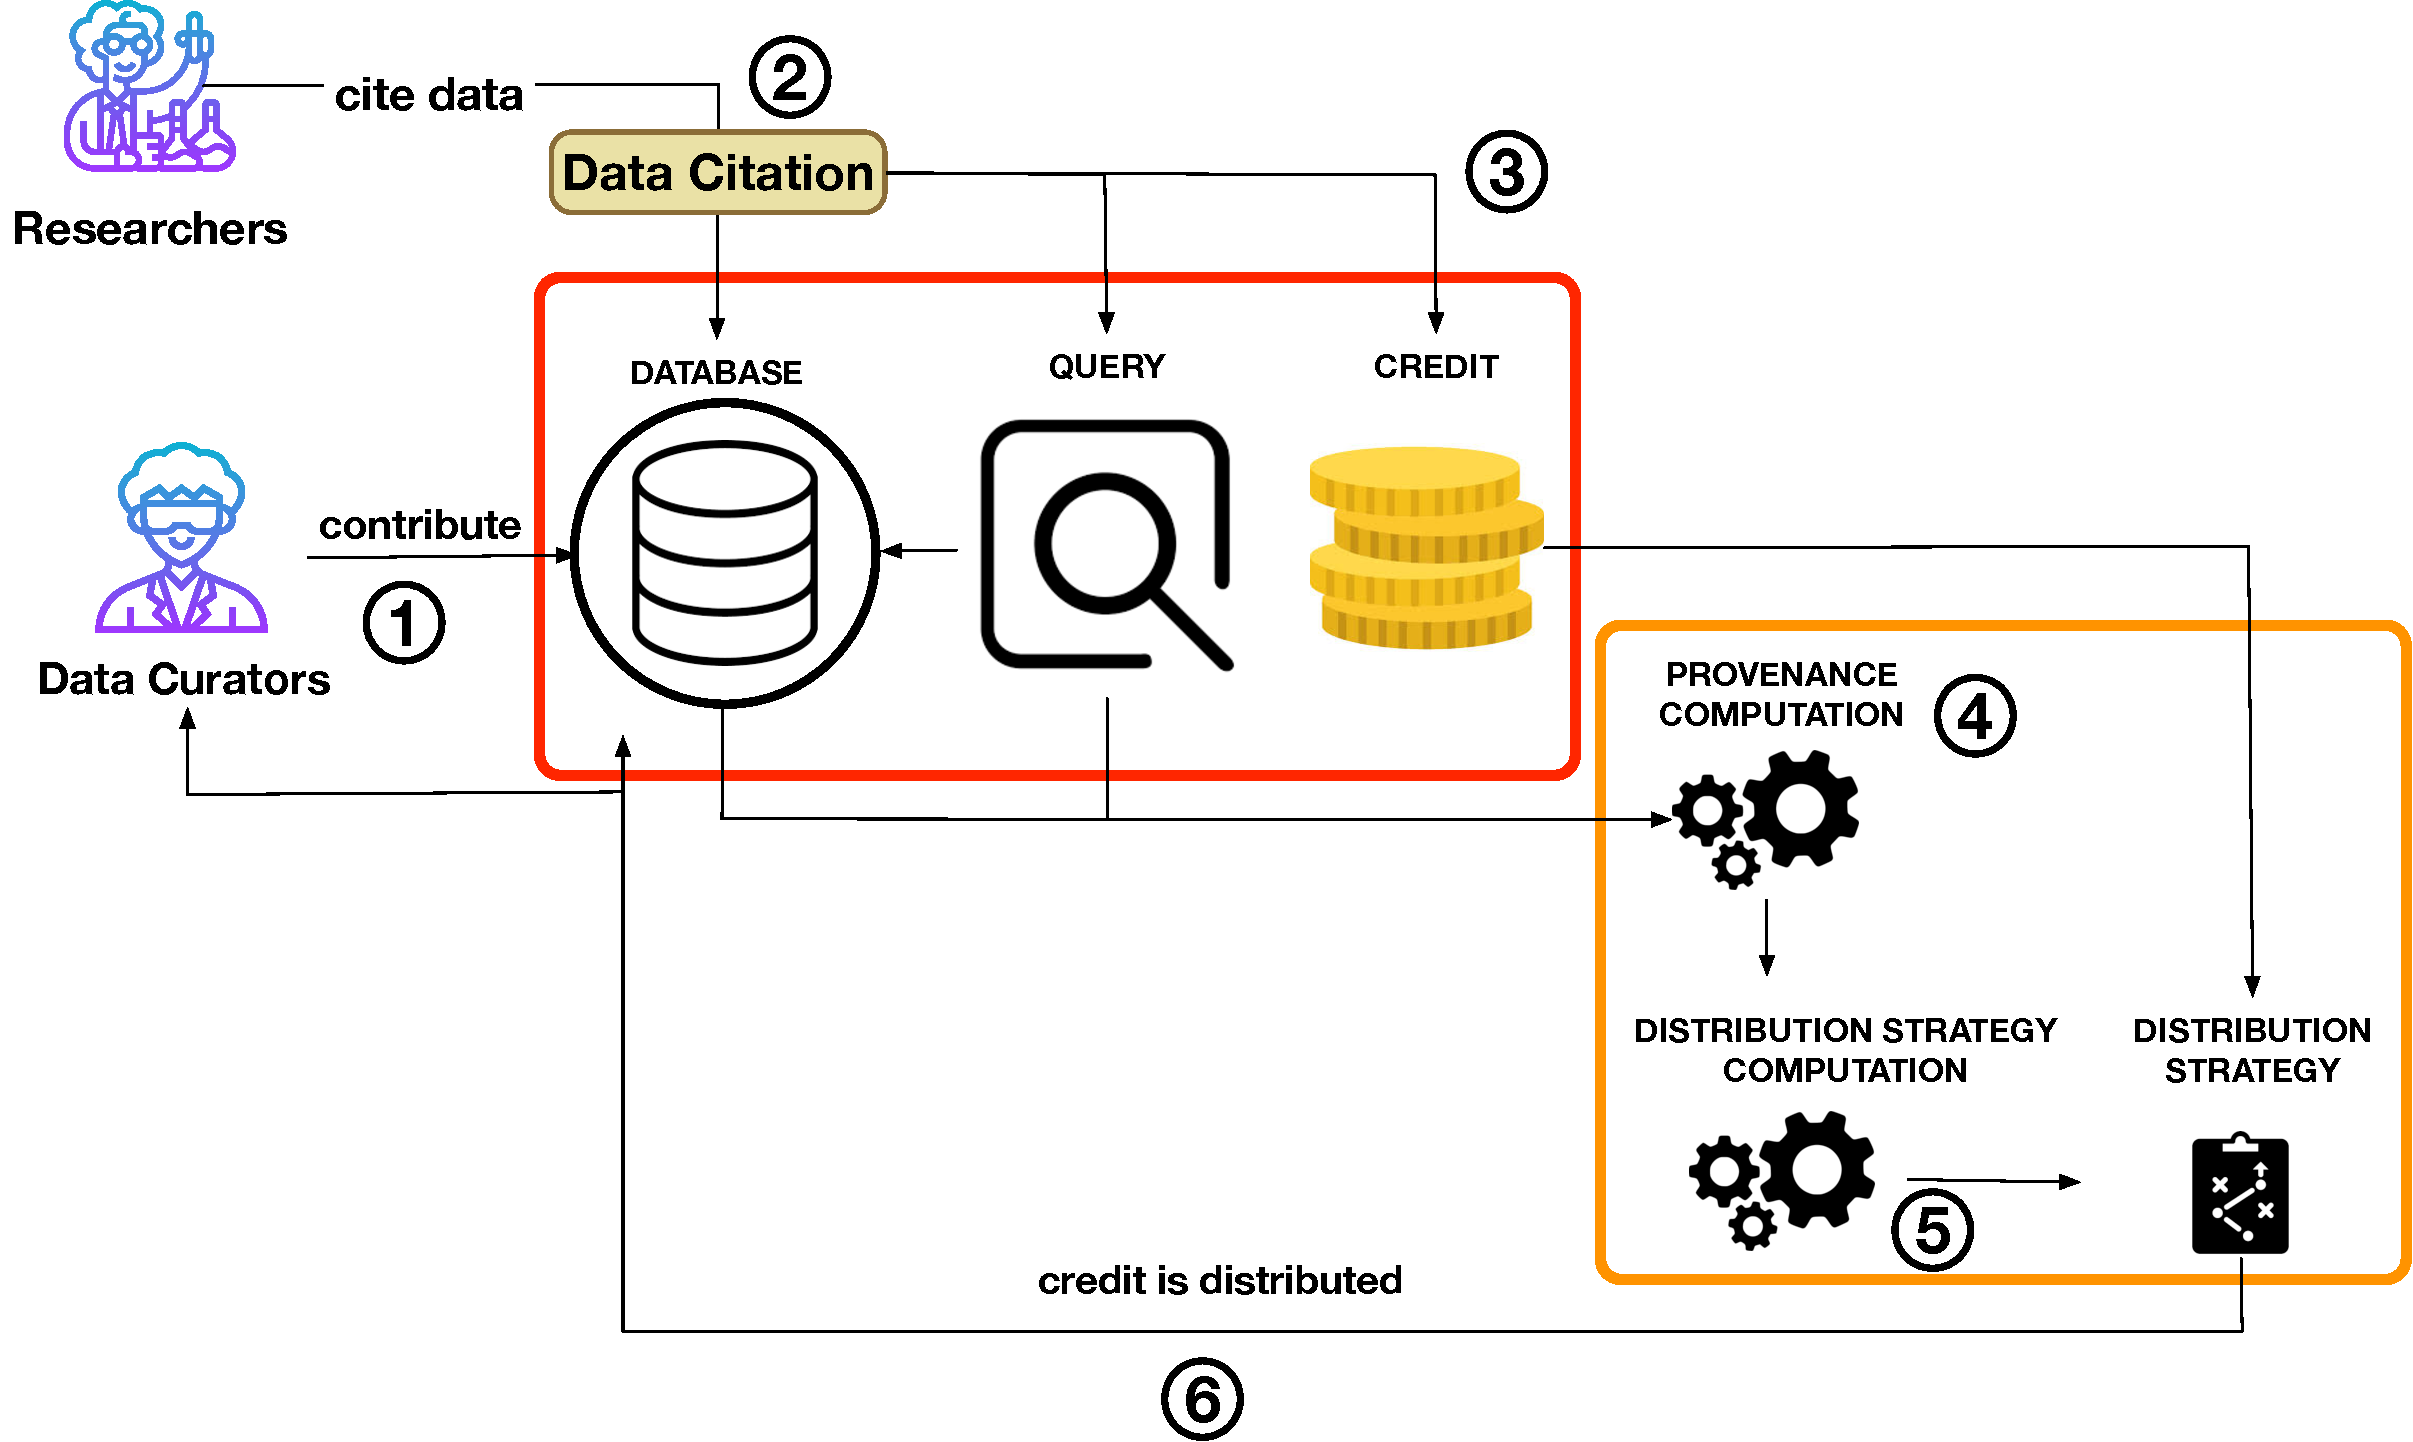
\includegraphics[width=.85\textwidth]{overview}
    \caption{Overview of the credit distribution pipeline.}
\label{fig:system_overview}
\end{figure}


% \scream{I find the description of this figure confusing. Is the assumption that this is a provenance enabled db which is capable of returning a citation along with the query result? So Step 2 is that the user issues a query that generates the data used, along with the citation?  Step 3 is then assuming the citation is used in a published paper, which generates some credit to the data used.  Step 4 now goes back in time to the db and query at the time it was asked, to calculate the provenance (or perhaps this is stored somehow), which is then used in Step 5 etc. }
\vspace{0.15in}
The DCD process that we use is summarized in Figure \ref{fig:system_overview}:
\vspace{0.15in}
\begin{description}
	\item[Step 1] Scientists and experts contribute 
	the curated information contained in a scientific database.  These are called the ``Data Curators".  
	\item[Step 2] Other researchers use the data in their research, and when possible, cite them. 
% 	\SBD{The rest of this Step is confusing. Rewrote. What dos it matter how researcheers access the data?  and the sentence was not complete.} 
	\item[Step 3] The citation to the data generates credit, that can be used as a proxy for the impact of the data on the citing paper. This credit is represented as a real value $k \in \mathbb{R}_{>0}$. 
	\item[Step 4] Given the database instance $I$ and the query $Q$,  the \emph{data provenance} of $Q(I)$ is computed. The data provenance of $Q(I)$ is a form of metadata that captures how 
	$Q$ used $I$ to generate the output~\citep{CheneyProvSurvey}. 
	\eat{, describing different kinds of relationships between data in the input and the output of a query. As reported in \citep{CheneyProvSurvey}, these provenances have been used in several applications beyond giving information on how queries work, for example, annotation propagation and the view update problem. }
	\item[Step 5] Provenance is input to the 
	\eat{DCD problem, whose aim is to compute the} \emph{Credit Distribution Strategy} (CDS, also referred only as Distribution Strategy, DS). CDS is a function $f$ that takes as input the credit value $k $, divides it and distributes it to the data in the input database $I$, and is defined on the basis of citation policies decided at the database administration level or at the domain community level. 
	%Since we are not in a "one-size-fits-all" setting, CDS can be defined with great variability and flexibility, thus allowing for ample customization. 
	\eat{In this paper, since we base CDS on data provenance, we describe four CDS, each one based on a different form of provenance. }
	\item[Step 6] Once the CDS is computed, it is used to distribute the given credit $k$ to the parts of the database that are responsible for the generation of $Q(I)$. Transitively, this credit is also divided and given to the corresponding authors of those data.
\end{description}

This paper expands the work in \citep{dosso2020data} %, which addressed the problem of how to reward data and data curators who are typically overlooked in current citation systems.
where we first defined the problem of DCD in relational databases, and proposed a viable Distribution Strategy (DS) based on \emph{lineage} -- the simplest form of \emph{data provenance}.
The lineage of a tuple $t$ in the output $Q(I)$ is defined as the set of all and only the tuples in the database instance $I$ that are ``relevant'' to the production of $t$.
% that is the tuple that are used by $Q$ in the production of $t$.
The corresponding strategy equally redistributes the credit $k$ to the tuples in the lineage set, thus each tuple receives credit $k/|L_t|$, where $L_t$ is the lineage set of $t$. 

One may argue that this DS is too simplistic, since lineage 
%only tells the relevant tuple used to produce the output, and 
does not convey any information about the role or importance of input tuples in the query.
Therefore, one may desire to give more credit to the tuples that are more {\em important} to the production of the output, i.e. those tuples that, if removed, would prevent the output tuple from appearing in the final result, or those tuples used more than once  by the query. 

Therefore, in this paper, we expand the ideas in \citep{dosso2020data} by proposing new DSs based on another form of data provenance:  how-provenance~\citep{howProvenanceGreen}.
We also propose other two DS based on the concepts of responsibility~\cite{MeliouGMS11} and the Shapley value~\cite{LivshitsBKS20,DFKM22}.
We discuss why one may be preferred to another depending on the application and its goals. 
% In particular, we show that the proposed new DSs are more sensitive than the lineage-based one to the {\em role} of a tuple in a query, i.e. how many times the tuple is used and how it is used. 
We also show that the DSs based on why-provenance and \rtwo{responsibility} give more credit to tuples that are essential to the production of the result set, whereas the how-provenance-based DS takes into consideration the different ways in which a tuple is used.
\rtwo{Finally, the DS based on the Shapley value sees the process of distribution as a competitive game in which tuples that contribute more to the generation of the output are correspondingly rewarded more.}. 
%\scream{Perhaps we could also say "Surprisingly, we also demonstrate that even the most complex DS, i.e.  the one based on Shapley, can be computed efficiently based on results in \cite{DFKM22}." Not sure if this should be "efficiently" or "quickly" as we are using it rather than proposing a new implementation. DD: not sure it needs to go here. In any case, it is said in the paper}

We use a well-known curated database called the IUPHAR/BPS\footnote{International Union of Basic and Clinical Pharmacology/British Pharmacology Society} Guide to Pharmacology~\citep{iuphar2018}, also known as GtoPdb\footnote{\url{https://www.guidetopharmacology.org/}}, to evaluate the DSs.  GtoPdb contains expertly curated information about diseases, drugs, cellular drug targets, and their mechanisms of action.
We chose GtoPdb for two main reasons: (i) it is a widely-used and valuable curated relational database, (ii) many papers in the literature use, and cite, its data (i.e., families, ligands, and receptors). 
Real queries used in papers can therefore be seen as data citations which, in turn, can be used to assign data credit.

We perform four sets of experiments. In the first, real queries are extracted from papers published in the British Journal of Pharmacology (BJP), that represent data citations to GtoPdb, and are used to distribute credit in the database using the three different provenance-based DSs. 
%We show how, given the peculiar nature of the queries, the three distributions do not present particular differences in this context and why this is the reason. 
In the second and third experiment we analyze the behavior of the different DS when complex citation queries are employed.
In the fourth set of experiments we use both real and synthetic queries to assess the difference between traditional citation and the notion of credit distribution in terms of rewarding those responsible for the data, e.g. data curators.

\textbf{Contributions}
 of this work include:
\begin{itemize}
    \item Three new Distribution Strategies based on how-provenance, responsibility and the Shapley value.
    \item An in-depth analysis of the effects of credit distribution on real-world curated data and of the differences between the five proposed Distribution Strategies.
    \item A comparison between the behavior of traditional citations and data credit in rewarding data curators.
\end{itemize}

\paragraph{\textbf{Outline}} The rest of the paper is organized as follows:
Section \ref{sec:related} presents background material and related work.   Section \ref{section:use_case} describes the GtoPdb use case. Section \ref{section:preliminaries} briefly presents the forms of provenance used in the paper.  Section \ref{section:distribution_strategies} describes the credit distribution problem and the proposed distribution strategies.  In Section \ref{sec:experiments} we present the experimental evaluation, followed by a discussion of our design decisions in Section~\ref{sec:discussion}. Section \ref{section:conclusions} draws some conclusions and outlines future work.

%############

\section{Background}
\label{sec:related}

\paragraph{Data in Research} %As described by Jim Gray in his last talk~\citep{hey2009jim}, 
The world of research is rapidly transitioning towards the \emph{fourth paradigm of science}~\citep{hey2009jim}, that is, data-intensive scientific discovery, where data are important for scientific advances as well as for traditional publications~\citep{Bechhofer2013linkisnotenough}.

The scientific community is promoting an \emph{open research culture}~\citep{nosek2015promoting}, founded on methods and tools to share, discover, and access experimental data. 
The community has identified the FAIR principles (Findable, Accessible, Interoperable, and Reusable)~\citep{fair2016Wilikinson}, that should be enforced by every database. 
In particular, data should be accessible from the articles, journals, and papers that cite or use them~\citep{cousijn2019bringing}.
Aspects such as the need for the \emph{reproducibility} of experiments through the used data; the \emph{availability} of scientific data; the \emph{connections} between data and the scientific results are all needed aspects for the fourth paradigm, and are all relevant to the domain of \emph{data citation}~\citep{honor2016data}.

\paragraph{Data Citation: Principles and Motivations} Data Citation principles were proposed in \citep{CODATA2013}, and later summarized and endorsed by the Joint Declaration of Data Citation Principles (JDDCP)~\citep{martone2014joint}. 
The principles are divided into two groups~ \citep{Silvello18jasist}. The first group contains principles concerning the role of data citation in scholarly and research activities such as the (i) \emph{importance} of data (why data citation is important and why data should be considered as first-class citizens); (ii) \emph{credit} and \emph{attribution} to the creators and curators of the data; (iii)\emph{evidence}; (iv) \emph{verifiability}; and \emph{interoperability}, with these last three requiring data citation methods to be flexible enough to operate through different communities. 
The second group defines the main guidelines to establish a data citation systems, and contains principles such as the (i) \emph{unique identification} of the data being cited; (ii) \emph{(open) access} to data; (iii) guarantee of \emph{persistence} and \emph{availability} of citations even after the lifespan of the cited entity; the (iv) \emph{specificity} of a citation, i.e. it must lead to the data set originally cited. 

The main motivations for data citation are outlined in~\citep{Silvello18jasist} and range from data attribution and connection to data sharing, impact and reproducibility. 

\eat{
\scream{SBD: Is the next paragraph necessary?  Could we just say "The main motivations for data citation are outlined in~\citep{Silvello18jasist}."}
\scream{GMS: yes. done}

It is possible to outline six main motivations for data citation~\citep{Silvello18jasist}:
\begin{itemize}
	\item \emph{Data attribution}: identify the individuals that should be credited for data with variable granularity.
	\item \emph{Data connection}: connect papers to the data being used.
    \item \emph{Data Discovery}: citations helps to find data records and subsets that would be otherwise not findable via search engines.
    \item \emph{Data Sharing}: share data obtained by researchers within the whole community. 
    \item \emph{Data Impact}: highlight the results obtained in writing papers using specific data, the frequency and modality data were used.
    \item \emph{Reproducibility}: data citation greatly impacts the reproducibility of science~\citep{baggerly2010disclose}. Many authoritative journals ask to share data and provide valid methodologies to reproduce experiments.
\end{itemize}
}

\subsection{Data Citation in Relational Databases}
%In this paper, we develop our methods and experiments on relational databases. 
Relational databases have been the target of data citation methods since the surge of the data-centric research paradigm. 
The RDA ``Working Group on Data Citation: Making Dynamic Data Citable''\footnote{\url{https://www.rd-alliance.org/groups/data-citation-wg.html}}~\citep{RauberEtAl2016} has developed guidelines for citing large, dynamic, and changing datasets which have now moved on into adoption phase. The datasets considered by the Working Group are often relational.

In one of its most recent sessions~\citep{rauber2015data}, the Working Group (WG) on Data Citation reported that there are various implementations of its guidelines for Data Citation on MySQL/Postgres relational databases. 
Some of these databases are: DEXHELPP\footnote{\url{http://www.dexhelpp.at/}} (Social Security Records); NERC (ARGO Global Array); EODC (Earth Observation Data Centre)~\citep{gosswein2019data}; LNEC (River dam monitoring); MDS (Million Song Database)~\citep{bertin2011million}; CBMI\footnote{\url{https://medicine.missouri.edu/centers-institutes-labs/center-for-biomedical-informatics}} (Center for Biomedical Informatics); VMC (Vermont Monitoring Cooperative); CCA\footnote{\url{https://ccca.ac.at/startseite}} (Climate Change Center Austria); VAMDC (Virtual Atomic and Molecular Data Center)~\citep{Dubernet_2016, ZwolfEtAl2016}.

More examples of work on data citation in relational databases are~\citep{bunemann2016citation, WuSIGMOD18, AlawiniDHW17,davidson2017model}. 
The website \texttt{\url{https://fairsharing.org/}} keeps an updated list of curated and scientific databases (many of which are relational or graph-based) following FAIR guidelines. These databases are citable since they are compliant with the most recent guidelines, and they are in the vast majority of cases accessible via dynamically created Webpages. 
In all these databases it is, therefore, possible to implement DCD on top of the existing infrastructures for citing data.

Data citation techniques are primarily applied to relational databases because of their pervasiveness as well as the ``identifiability" of the portions of data that are to be cited: the whole database, a relation, a tuple, or even an attribute. 
Many papers \citep{buneman2006cite, bunemann2016citation, AlawiniDHW17} consider more complex citable units, recognizing that often the \emph{views} of a database are the ones to be cited. Generally, a \emph{view} is a query on the database.
To this end, \citep{WuSIGMOD18} suggested decomposing the database into a set of views, where each view is associated with its citation. 


At present, the most common practices to cite databases include:
\begin{enumerate}
    \item A database cited as a whole, even though only parts of the databases are used in the papers or datasets. Alternatively, the so-called ``data papers'' are cited, being traditional papers that describe a database~\citep{CandelaEtAl2015}. \\
    In this case, all the credit from the citations goes to the database administrators or to the authors of the data papers. 
    \item Subsets of data, obtained by issuing queries to a database, are individually cited. This is the solution adopted by the \emph{Resource Data Alliance} (RDA) working group on Data Citation~\citep{RauberEtAl2016}.
    In this case, the credit generated from citations is distributed among the contributors of the portions of data being cited, and/or to the database administrators. 
    \item The database is accessible via a series of Webpages that arrange the content of the database by topic or theme. Examples in the life science domain include the Reactome Pathway database~\citep{reactome2016}, the GtoPdb \citep{iuphar2018}, and the VAMDC~\citep{ZwolfEtAl2016}.
     Every single Webpage is unequivocally identifiable and can be individually cited. 
\end{enumerate}

\eat{
\textcolor{red}{Despite all the research efforts dedicated to the study and promotion of data citation, none of the largest citation-based systems, such as Elsevier Scopus, Web of Science, Microsoft Academia, or Google Scholar, consider scientific datasets as citable objects in academic work. 
Clarivate Analytics Data Citation Index (DCI) \citep{force2016research} is an exception, since its infrastructure tracks data usage in scientific domains and provides the technical means to connect datasets and repositories to scientific papers. However, DCI considers only citations to (previously registered and approved) databases as a whole and does not count citations to database portions such as views, tables, or tuples.}
\scream{GMS: I'd remove (eat env.) this part about citation-based indexes because we are not proposing any solution for that problem.}
}

%Scholix
%Publishers, data centers, and indexing services have started to create bidirectional links between research data and scholarly literature. Such links, however, usually stem from agreements implemented by two organizations. They, therefore, lack a universally accepted industrial standard, and each agreement differs from the other~\citep{burton2017scholix}. 
%The rapid growth of bilateral agreements hinders interoperability, which is one of the principles of data citation. In fact, this kind of agreement has generated a series of undesirable side-effects. Many publishers, data centers, repositories, and infrastructure providers remain disconnected.
%Moreover, the heterogeneity that ensues from (considerably different) agreements and practices hinders the global interoperability among different agreements. 
%One example of such heterogeneity may be found in identification systems such as Digital Object Identifiers\footnote{\url{https://www.doi.org}} (DOI) and Life Science Identifiers\footnote{\url{http://www.lsid.info}} (LSID).
%
%The Scholix framework \citep{burton2017scholix} addresses this issue. As a community and multi-stakeholder driven effort, it strives to facilitate information exchange between data and literature and between data and data. 
%It can be regarded as a framework, a set of guidelines, and lightweight models to facilitate interoperability among link providers. 



\subsection{Data Credit}
Data credit is related to data citation: they both aim to recognize the work of data creators and curators. 
Data credit can therefore also be seen as a by-product of data citation, since credit attribution is impossible without the presence of data citations.

\citet{transitiveCreditKatz2014} suggests the need for a \emph{modified citation system} that includes the idea of \emph{transient} and \emph{fractional credit}, to be used by developers of research products as software and data.
Two considerations are made: (i) research objects such as data and software are currently not formally rewarded or recognized by the community; 
(ii) even in traditional papers, the contribution of each author to the work is hard to understand, unless explicitly specified in the paper. 
This is even more true for data, where different groups of people work on the same database.

In \citep{transitiveCreditKatz2014} credit is defined as a ``quantity'' that describes the importance of a research entity, such as papers, software, or data, mentioned in a citation. 
It also proposed the idea of a \emph{distribution} of credit from research entities, such as papers or data, to other research entities through citations. 
Therefore, when discussing data credit, we need to consider  \emph{credit computation} -- i.e., the process to compute the quantity of credit generated by the citation -- and \emph{credit distribution} -- i.e., the process to distribute credit and to assign it to the entities that contributed to the creation/curation of the cited data. In this paper we focus on the latter.

These two processes are done by exploiting the structure of the \emph{citation graph}, a directed graph whose nodes are publications and edges are citations.
This graph is the model at the core of systems such as Google Scholar and the Web of Science.
We add to this that the concept of credit can be built on top of the existing infrastructure handling traditional and data citations.

\citet{transitiveCreditKatz2014} further explores the idea of a \emph{distribution} of credit from research entities (i.e., papers and data) to other research entities through citations that connect them. 
Thanks to traditional citations and now also to data citations, this distribution is finally possible, at least between papers and data. 
Some problems related to traditional citations can thus be solved by citations:

\begin{enumerate}
\item Credit rewards research entities that to date are not (formally) recognized (a goal shared with data citation).
\item Credit can reward authors \emph{proportionally} to their role in generating the entity. The more an author contributes to a paper, the more credit is given to him. \citet{ZouP16} work on something similar with their zp-index, which includes in its formulation the position (and thus the role) of a publication author to represent its impact in the work itself.
\item Credit can be \emph{transitively} channeled through a chain of papers citing each other, thus enabling the rewarding of older papers that are no more cited, since other papers summarize or report their content 
%\textbf{Gianmaria: I do not understand this token, what do you mean with: papers that are no more cited?} 
but are nevertheless crucial in a research area for the influence of their content.
\end{enumerate}

\citet{creditFang18} presents a framework to distribute the credit generated by a paper to its authors and to the papers in its reference list in a transitive way. 
Let us consider the \emph{citation graph} as the graph where the nodes are papers and the links are the citations among them.
In this graph, every paper is a source of credit, which is then transferred to the neighboring nodes.
The quantity of credit received by each cited paper depends on its impact/role in the citing paper. 
So far, this theoretical framework is limited to papers, but it can be easily extended to a citation graph including both papers and data. 

\citet{zeng2020assigning} proposes the first method to compute credit within a network of papers citing data. 
Adopting a network flow algorithm, they simulate a random walker to estimate a score for each dataset, leveraging real-world usage data to compute the credit.
This is the first step towards an automatic credit computation procedure.
This proposal is, however, limited to assigning credit to whole datasets, and it does not deal with the granularity of data. It does not work to assign credit to a single research entity within a dataset. 
Differently from \citet{zeng2020assigning}, we do not treat the credit computation process, but we focus on the distribution process.

%%%%%%%%%%%
\subsection{Data Provenance}
\label{section:related_provenance}

To distribute credit, we base two of our methods on \emph{data provenance}. 
Data provenance is information that describes the origin and the process of creation of data. It can also be seen as metadata pertaining to the derivation history of the data. 
It is particularly useful to help users to understand where data are coming from, and the process they went through. 
Data citation and data provenance are closely linked~\citep{AlawiniDSTW17} since both are forms of annotations on data retrieved through queries. 
Data provenance has been widely studied in different areas of data management. 
In this paper, we focus on provenance for database management systems (DBMS). For further details on data provenance, please refer to surveys like \citep{CheneyProvSurvey} and \citep{SimmhanPG05}.

\citet{CheneyProvSurvey} presents four main types of data citation for DBMS: \emph{lineage}~\citep{lineageCui}, \emph{why-provenance}~\citep{WhyProvBuneman}, \emph{how-provenance}~\citep{howProvenanceGreen} and \emph{where-provenance}~\citep{WhyProvBuneman}.

Let us start with the first three provenances. Given a database instance $I$, a query $Q$, and the result $Q(I)$, consider one tuple $t$ of the output. 
Its provenance is information about its generation through the tuples of the input that are used by $Q$. Different types of provenance convey different levels of information. Since these three provenances are computed for each tuple of the output, they are also referred to as \emph{tuple-based}.

%Lineage is the simplest among the forms of provenance. It has been defined in different ways~\citep{CheneyProvSurvey}, but it can be thought of as the set of all the tuples that are used in some way by the query to produce the output tuple, the ones that are somehow \emph{relevant} to its generation. 
%
%The definition of why-provenance is based on the notion of \emph{witness set}. A witness is a set of relevant tuples that guarantees the existence of $t$ in $Q(D)$. The lineage is therefore an example of a witness. The why-provenance of a tuple $t$ is a peculiar set of witnesses  -- described in \citep{WhyProvBuneman} -- that are computed from the query, called \emph{witness basis}. 
%A witness basis may be composed of more than one witness. 
%Therefore, the why-provenance contains more information than the lineage, since it describes \emph{alternative} ways in which the same output may be generated. 
%
%The how-provenance takes the form of a polynomial, called \emph{provenance polynomial}, where the variables are taken from the set of identifiers of the tuples (provided that each tuple in $I$ has an identifier) and the coefficients are drew from $\mathbb{N}$. 
%This provenance also contains information on \emph{how} the input tuples are used. For example, when two tuples are combined by a join, they are also combined in the polynomial by the $\cdot$ operator. When two or more tuples become equivalent due to a union or a projection, the corresponding monomials are combined by the $+$ operator.
%
%It has been shown in \citep{CheneyProvSurvey} that the how-provenance is the more general and informative of the three, containing the other two.

Where-provenance, differently from the other three, is \emph{attribute-based}, so we do not take it into account in this work since we consider the tuple as the finest citable unit. 

\subsection{Causality and Responsibility}
We also consider the notions of causality and responsibility, as defined in 
\cite{MeliouGMS11}. Causality is an enrichment of lineage, and it is the attribution of a certain degree of importance to the tuples of the lineage based on their role in the generation of the output. Responsibility is a value given to the tuples of the lineage to rank them based on their degree of causality (the more important the role of a tuple in generating the output, the higher its responsibility).

While computing responsibility for general queries is hard~\cite{ChocklerH04}, \citet{MeliouGMS11} proved a dichotomy result for conjunctive queries: for each query without self-joins, either its responsibility can be computed in PTIME in the size of the database or checking if it has a responsibility below a given value is NP-hard.

\subsection{Shapley value}
The Shapley value was introduced in 1952~\cite{Shapley1954}, framed as a \emph{cooperative game} played by a set $A$ of players, and defined by a \emph{wealth function} $v$ that assigns to each coalition set $B \subseteq A$ the wealth $v(B)$.
The question behind the Shapley Value is how to quantify the contribution of each player to the overall wealth. 
Informally, the Shapley value is defined as follows~\cite{LivshitsBKS20}: assume that we select players randomly one by one and without replacement, starting with the empty set. Every time a player $a$ is selected, its addition to the coalition $B$ produces a change in the wealth of the coalition from $v(B)$ to $v(B \cup \{a\})$. The Shapley value of $a$ is the expectation of change that $a$ causes in this probabilistic process.

The Shapley value has been widely used, e.g. in economics, law, environmental science, and network analysis, and has strong theoretical justifications. However, its use in databases as a metric for quantifying the influence of a tuple on the output of a query (thereby presenting an alternative to responsibility)  has only recently been considered~\cite{LivshitsBKS20}. 
The initial theoretical analysis in \cite{LivshitsBKS20} showed mainly lower bounds on the complexity of the problem, and did not suggest a feasible implementation.
However, very recently, an efficient implementation for Boolean queries has been provided~\cite{DFKM22}, both in terms of an exact computation (which in practice works well for most queries) and in inexact one (which is extremely fast and provides the same ranking of tuples as the exact computation, but not necessarily the same values).


\section{Use Case: GtoPdb}
\label{section:use_case}

\begin{figure}[t]
\centering
  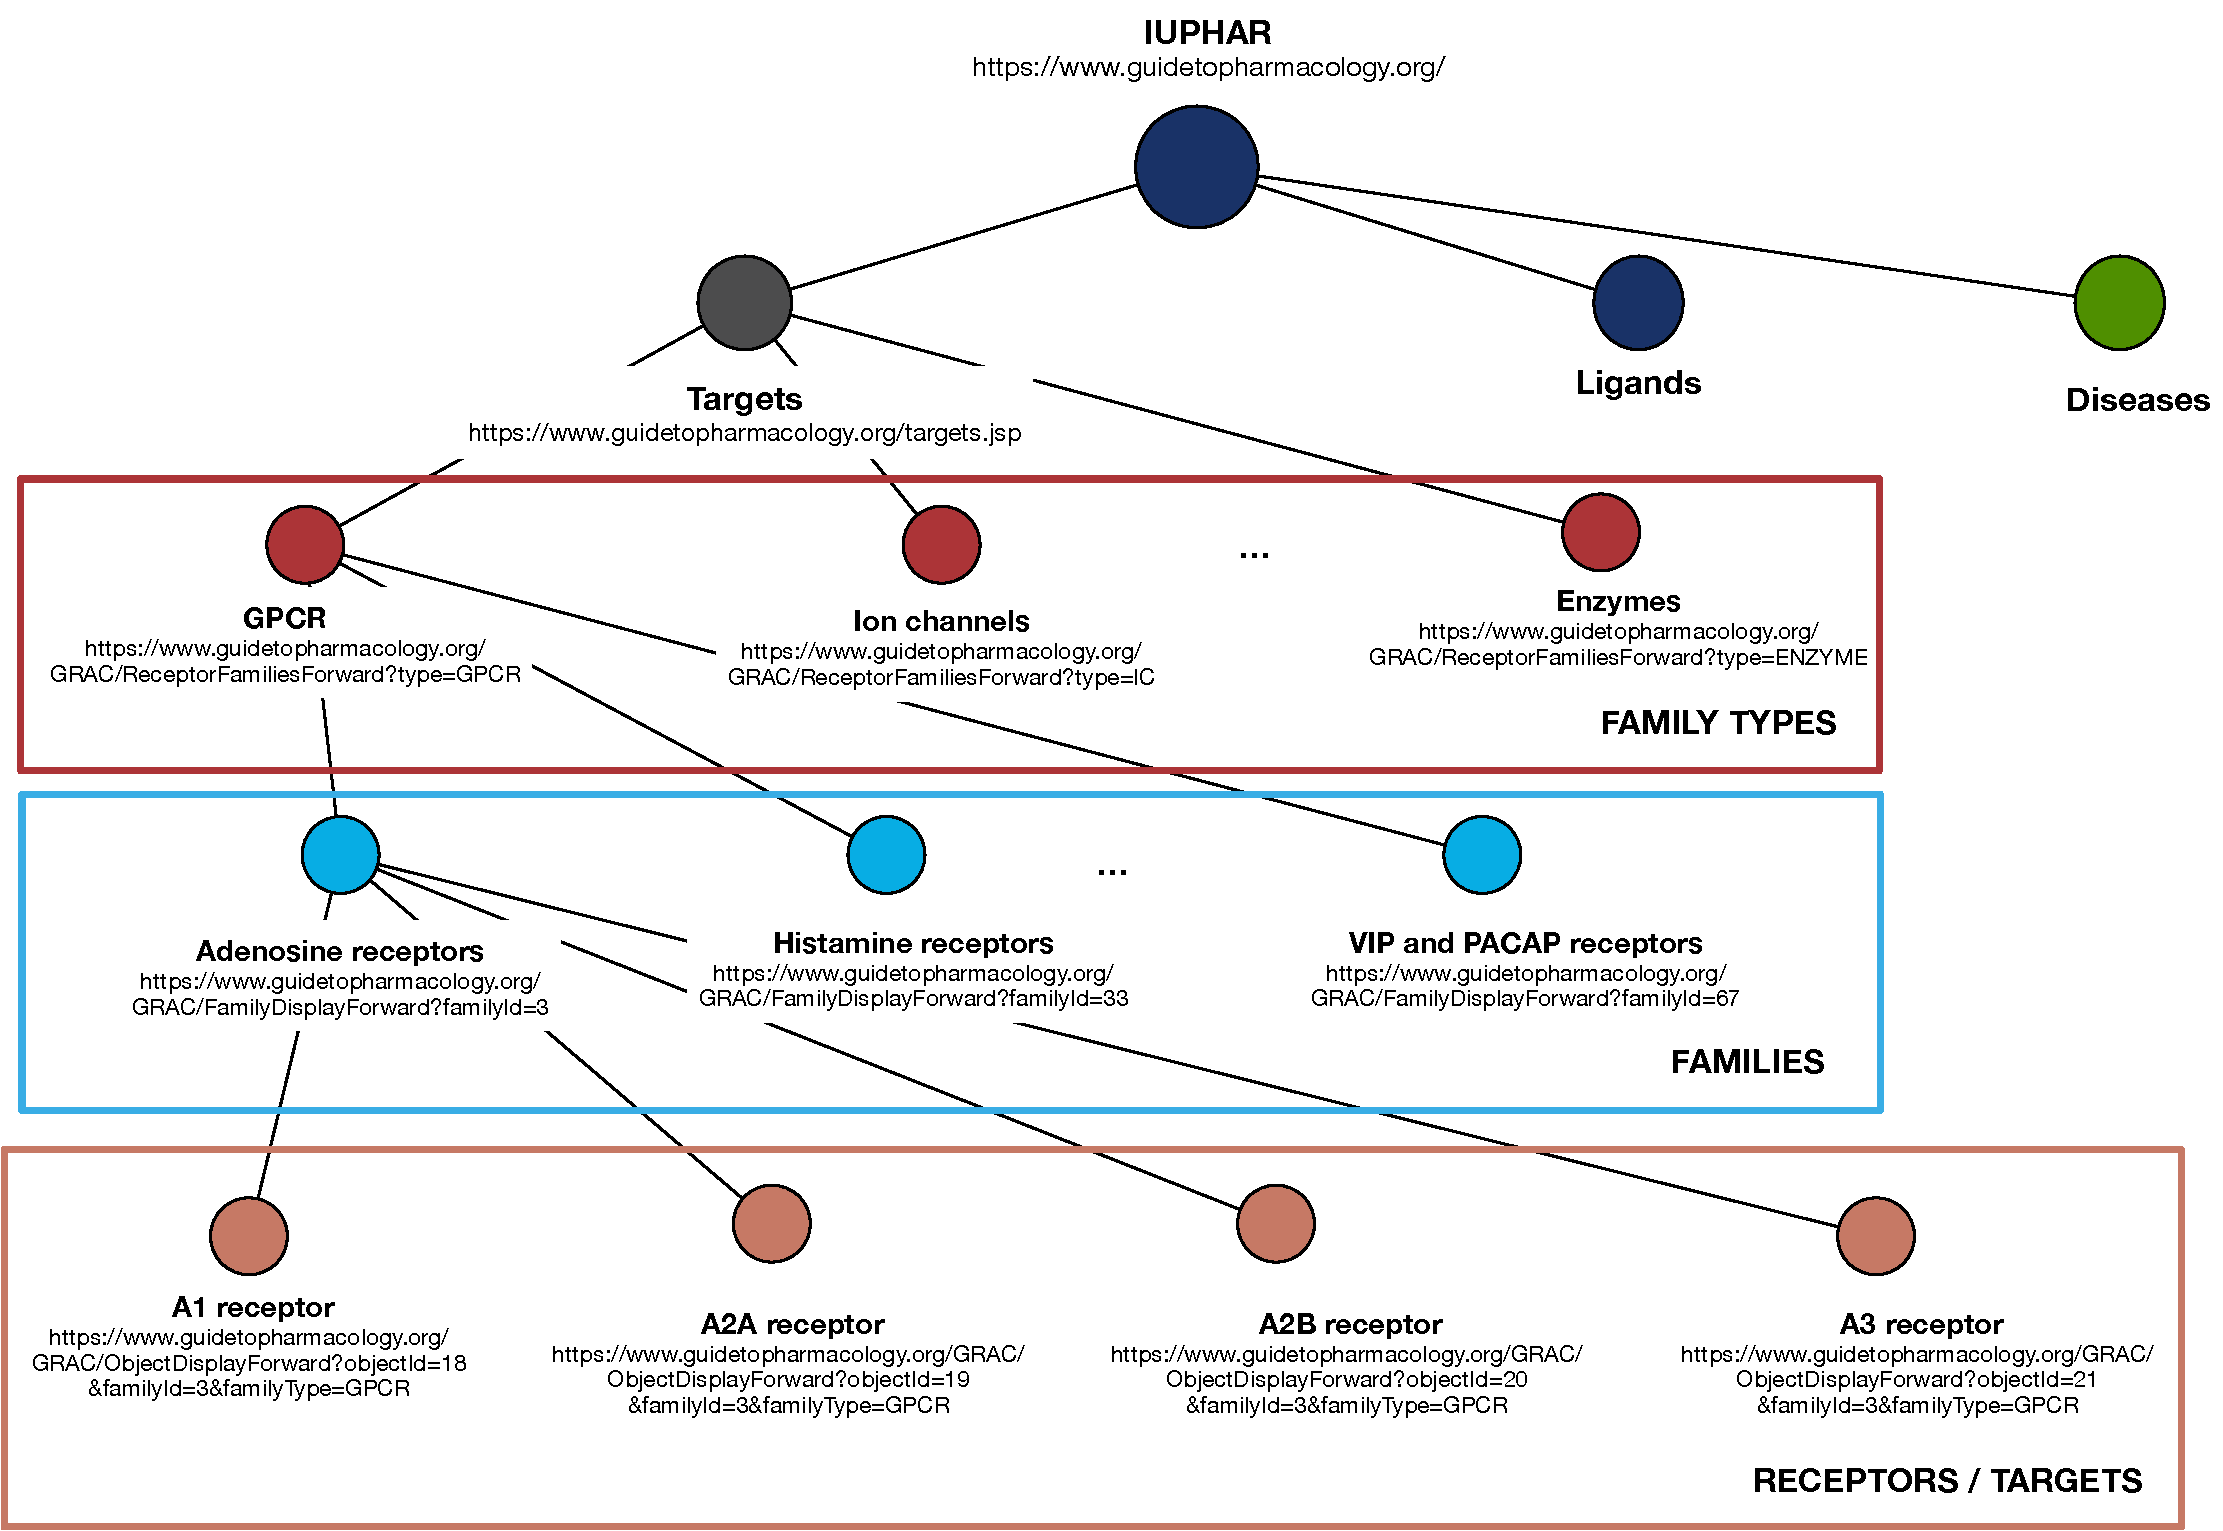
\includegraphics[width=.9\textwidth]{iuphar_schema}
  \caption{Partial map of the GtoPdb hierarchical structure grouping the targets into families and family types.}
  \label{figure:iuphar_schema}
\end{figure}

The IUPHAR/BPS Guide to Pharmacology \citep{iuphar2018}  (GtoPdb\footnote{\url{https://www.guidetopharmacology.org/}}) is a well-known and well structured scientific relational database that contains expertly curated information about diseases, drugs in clinical use, their cellular targets, and the mechanisms of action on the human body. 
It is curated and maintained by the GtoPdb Committee and 96 subcommittees, comprising 512 scientists collaborating with in-house curators who draw the information contained in the database from high-quality pharmacological and medicinal chemistry literature.
Roughly $1000$ researchers from all over the world have contributed to the database, and the curators wanted to give recognition to these contributors.  This led to some early work on data citation~\citep{buneman2006cite}.  

GtoPdb is relational, but its logical structure is hierarchical as shown in Figure \ref{figure:iuphar_schema}.  The information contained in the database is also organized into webpages focused on specific diseases, targets or ligands, and families % (i.e., groups) of them 
for easier access by users. 
As depicted in Figure \ref{figure:iuphar_schema}, the database can be thought of as a tree where the root is the database; the first level consists of all targets, ligands, and diseases; and the lower levels consists of specific targets, ligands and diseases. 
In this paper, we focus on targets; thus the figure at the third level shows examples of family types, at the fourth level of specific families of targets (a finer level of granularity), and finally, at the last level, the single targets (also known as receptors). 

\begin{figure}[t]
\centering
  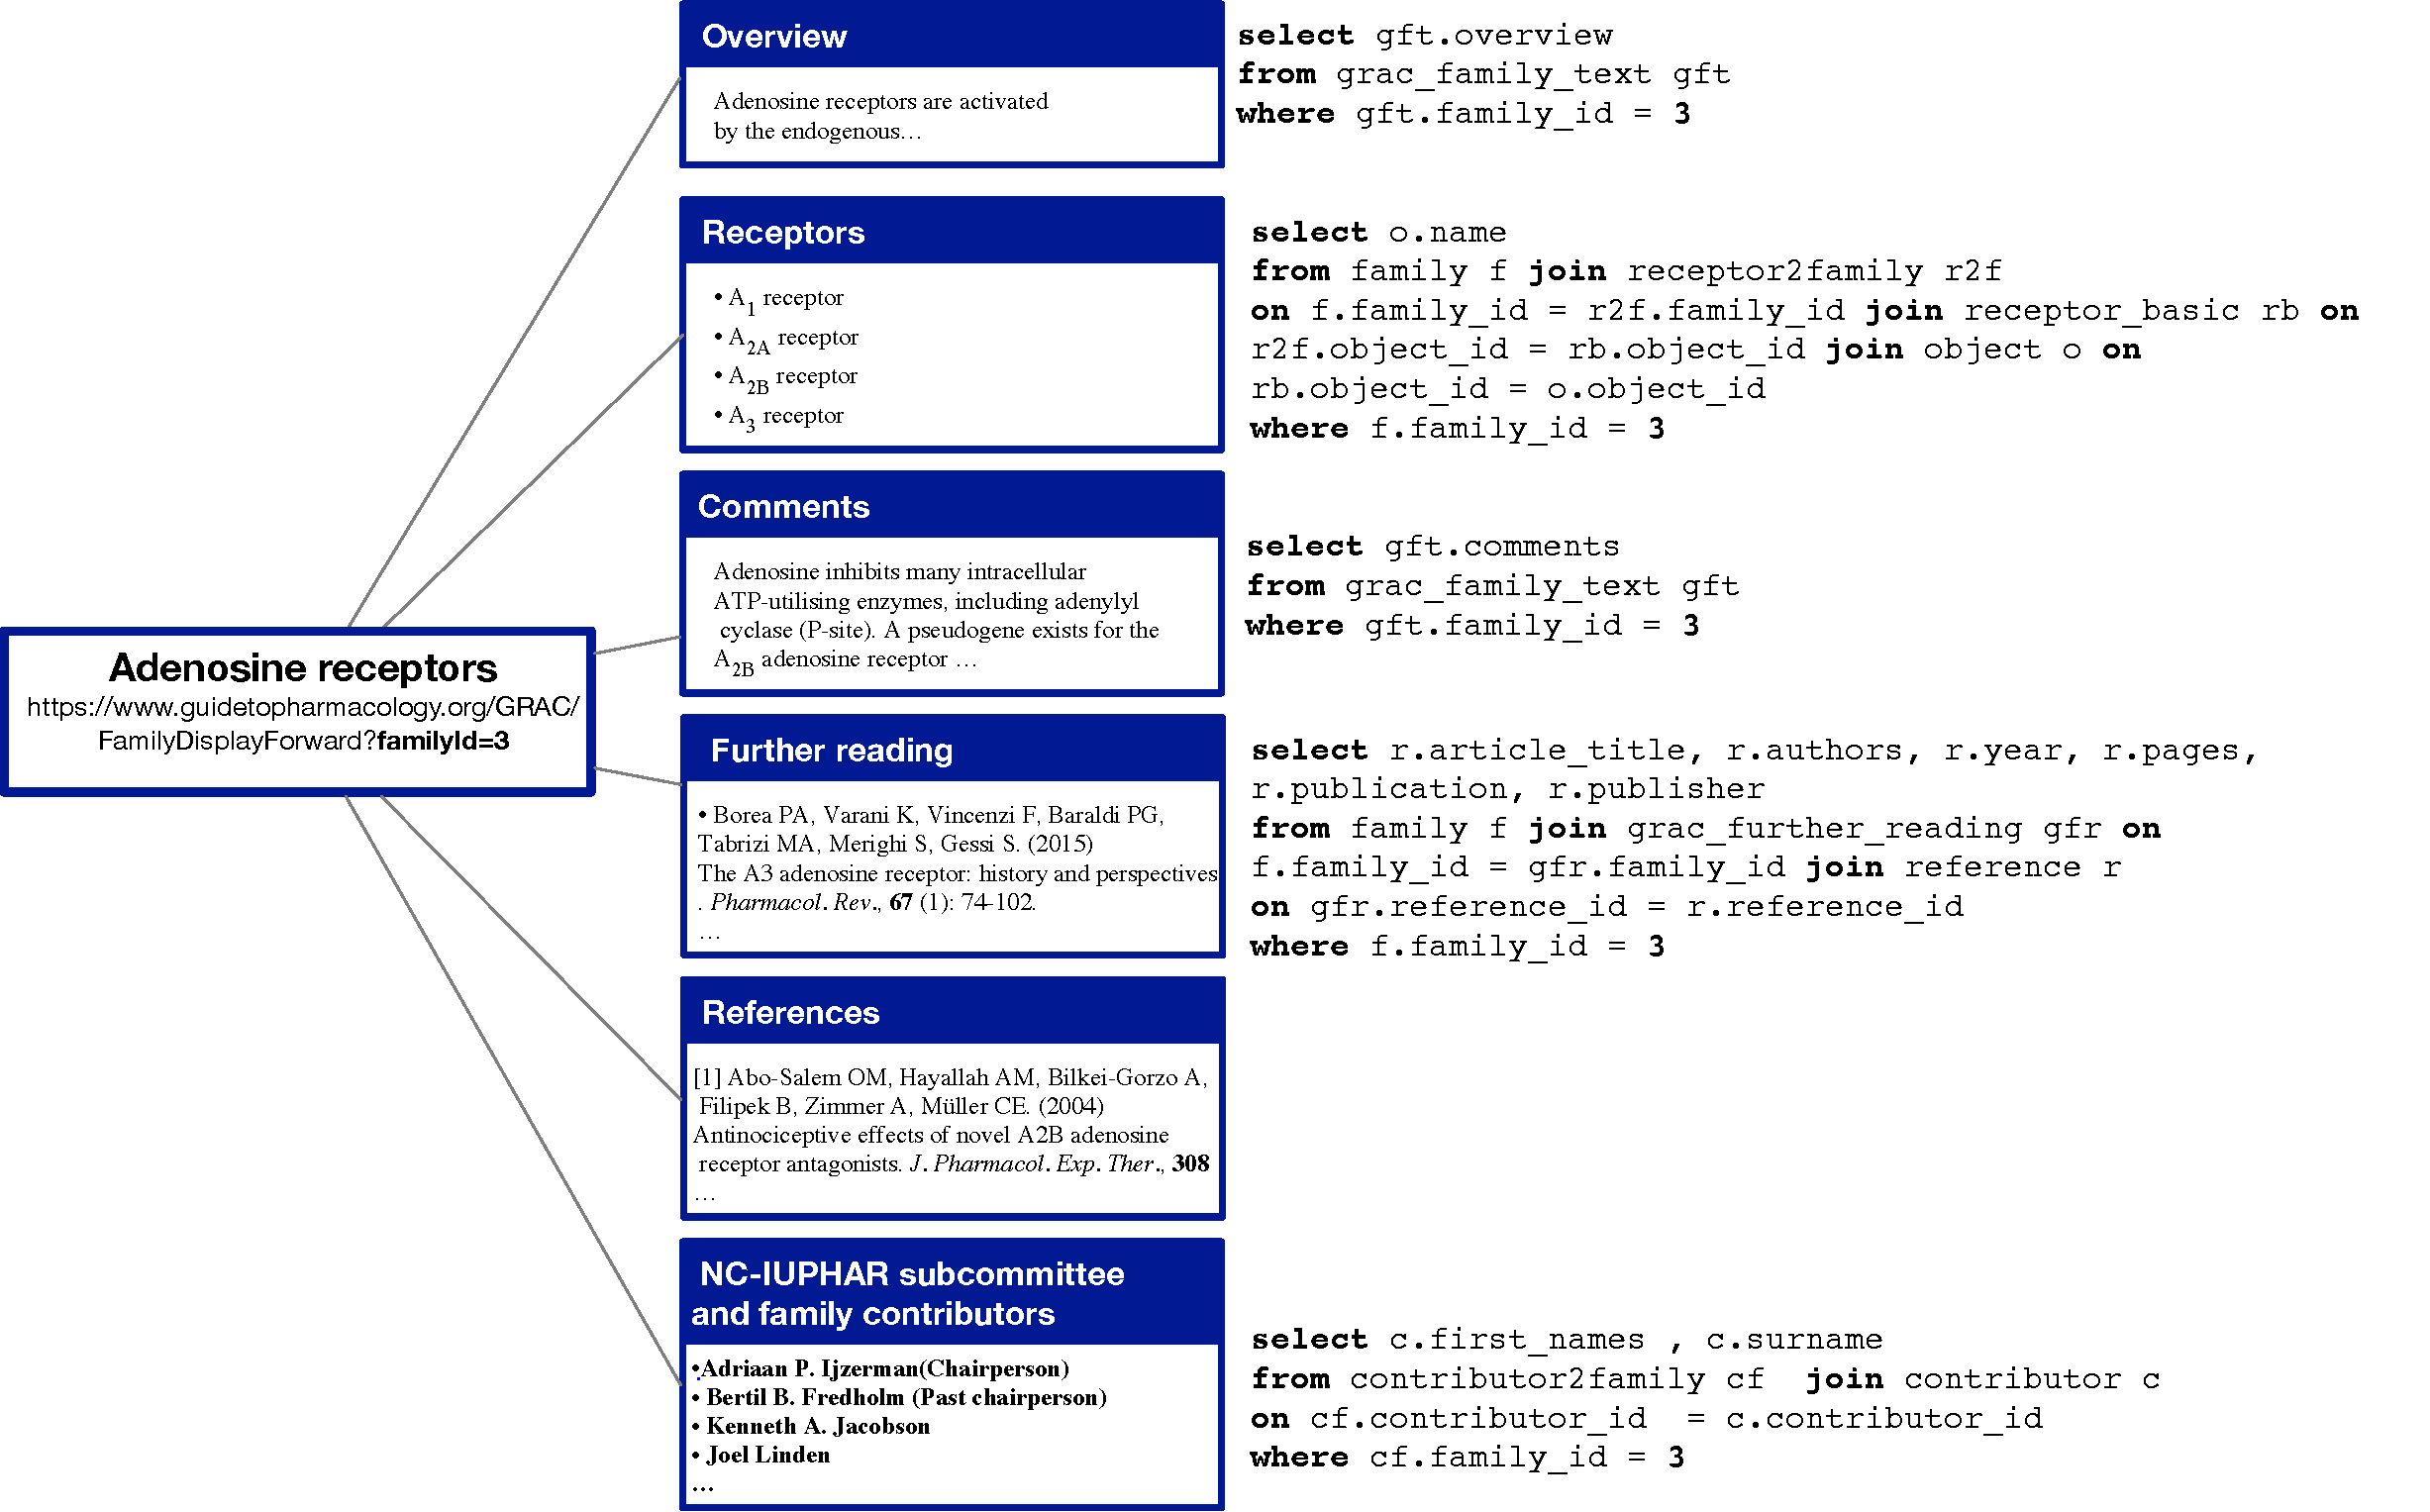
\includegraphics[width=1\textwidth]{family_structure}
  \caption{Basic web-page structure of ``Adenosine receptors'' family (ID 3), with queries used to retrieve the information contained in every section, except references.}
  \label{figure:family_structure}
\end{figure}


GtoPdb provides access to the webpages corresponding to all these nodes through URLs. 
The webpages corresponding to target families all present a similar structure, as shown in Figure \ref{figure:family_structure} for the ``Adenosine receptors'' family. 
Each page has an \emph{Overview}, a brief text describing the content of the page; a list of \emph{Receptors} comprising the family; a section of \emph{comments} about the family;
the \emph{References}, a list of the papers consulted by the curators of the page, similar to a reference list of a paper;
the \emph{further reading} list, reporting papers that an interested reader may want to consult to obtain more insight on the family; and a final section called \emph{How to cite this family page}, containing text snippets useful to cite the specific page or the whole database. 
Figure \ref{figure:family_structure} shows the SQL code that retrieves the information used to build the corresponding sections (apart from the References section).
Therefore, each family page can be considered a full-fledged traditional publication, consisting of title, authors, abstract (the overview), content, and references. 

In practice, many papers in the literature only reference GtoPdb (the root) without including a reference to the specific page being cited. 
That is, they only cite a paper describing GtoPdb as a whole (e.g., \citep{iuphar2018}) and refer to targets, ligands, diseases, etc. only by name. 
Thus, citations to specific families are \emph{de-facto} ``hidden'' to citation systems such as Google Scholar, and useless for the computation of bibliometrics. 

In certain ``lucky'' cases, as with papers available in PDF and published in the British Journal of Clinical Pharmacology~\footnote{\url{https://bpspubs.onlinelibrary.wiley.com/journal/13652125}} (BJCP), when a  family, ligand, receptor name, etc. are used, they have a hyperlink pointing to the corresponding webpage in GtoPdb. Therefore, the citations to the families can be detected and counted using the URLs reported in the papers.
However, these citations to GtoPdb webpages are not counted as such by citation systems, so they are not converted into credit for curators and collaborators. 

For our running example, consider Table \ref{table:running_example}. This simplified version of GtoPdb contains three tables: \texttt{family}, \texttt{contributor} and \texttt{contributor2family}.
% \scream{You have an id column which is "separate" from the other attributes in table.  Are these introduced as provenance tokens, or are they real attributes?  Later you speak about introducing an id in the query result, is this the same?}
The first table, \texttt{family}, has tuples representing families with three attributes: the id of the family, its name, and type. 
Table \texttt{contributor} contains people who have helped generate the data in the database.
The third table, \texttt{contributor2family}, serves as a link between the families and the people who contributed to them.
For instance, ``John Smith'' ($\mathtt{c_1}$) contributed to ``Dopamine Receptors'' ($\mathtt{f_1}$) as well as to the ``YANK Family'' ($\mathtt{f_4}$). Throughout the rest of the paper, we will use the \texttt{id} attribute of these tables as the \emph{provenance token} of its corresponding tuples, that is, as a symbol that serves to identify a tuple when talking about provenance.

\begin{table*}[]
\centering
\begin{tabular}{| l | cc |}
\multicolumn{3}{c}{\textbf{family}}\\
\hline
 id & name & type \\
  \hline
  $f_1$ & Dopamine Receptors & gpcr \\
  $f_2$ & Bile Acid Receptor & gpcr \\
  $f_3$ & FAK Family         & enzyme \\
  $f_4$ & YANK Family        & enzyme \\
\hline
\end{tabular}	
\begin{tabular}{| l |c c|}
\multicolumn{3}{c}{\textbf{contributor2family}}\\
\hline
 id & family\_id & contributor\_id \\
  \hline
  $c2f_1$ & $f_1$ & $c_1$ \\
  $c2f_2$ & $f_1$ & $c_2$ \\
  $c2f_3$ & $f_2$ & $c_3$ \\
  $c2f_4$ & $f_4$ & $c_1$ \\
\hline
\end{tabular}		
\begin{tabular}{| l |c c|}
\multicolumn{3}{c}{\textbf{contributor}}\\
\hline
 id & Name & Country \\
  \hline
  $c_1$ & John Smith & UK \\
  $c_2$ & Jim Doe & UK \\
  $c_3$ & Hans Zimmerman & Germany \\
  $c_4$ & Roberta Rossi & Italy \\
\hline
\end{tabular}		
\caption{Example of a database consisting of three tables. \texttt{family} contains receptor families; \texttt{contributor} contains the name and country of contributors; \texttt{contributor2family} connects contributors to the families they contributed to.}
\label{table:running_example}
\end{table*}

\section{Provenance, Responsibility, and Shapley}
\label{section:preliminaries}

\begin{table}[]
    \centering
%    \caption{\rone{Notation used in Definition \ref{def:how_distribution}.}}
    \begin{tabular}{c|c}
    \hline
    	 $I$ & database instance \\
    	 $L_t$ & lineage set of an output tuple $t$ \\
    	 $\Gamma$ & contingency set \\
    	 $\rho_t$ & responsibility of tuple $t$ \\
    	 $Q$ & a query \\
    	 $\bar{Q}_{o}$ & Boolean query such that $\bar{Q}_{o}(I) = 1$ if $o$ is present in $Q(I)$ \\
    	 $\mathcal{W}$ & witness basis \\
    	 $W$ & a witness set \\
    	 $\gamma(\mathcal{W}, t)$ & set of witnesses in $\mathcal{W}$ containing $t$ \\
         $\mathcal{H}$ & provenance polynomial  \\
         $M_i$ & a monomial in $\mathcal{H}$ \\
         $t_j$ & a tuple in $M_i$ \\
         $c(\mathcal{H})$ & sum of $\mathcal{H}$'s coefficients \\
         $e(M_i)$ & sum of $M_i$'s exponents \\
         $mc(M_i)$ & $M_i$'s coefficient \\
         $te(t_j, M_i)$ & exponent of $t_j$ in $M_i$ \\
         $\gamma(t_j, \mathcal{H})$ & set of monomials in $\mathcal{H}$ containing $t_j$ \\
    \hline
    \end{tabular}
   \caption{\rone{Notations used in this paper.}}    \label{tab:notation}
\end{table}


We now describe the notion of provenance used in this paper --  how-provenance -- as well as
the notion of causality and responsibility, and the Shapley value function. 

% \subsection{Lineage}
% \rone{Lineage is the simplest form of provenance. It was first introduced by \citet{lineageCui}, and can be thought of as the set of all tuples that
% %are \emph{relevant} (or that 
% are used by the query to generate the output~\cite{CheneyProvSurvey}.}


% As an example, consider the following SQL query \texttt{Q1}, applied to the database described in Table \ref{table:running_example}, asking for the names of families curated by researchers based in the United Kingdom (UK):

% \vspace{2mm}
% {\footnotesize
% \begin{adjustwidth}{25pt}{0pt}
% \begin{verbatim}
% 		Q1: SELECT DISTINCT f.name
% 		FROM family AS f JOIN contributor2family AS c2f 
% 		ON f.id = c2f.family_id
% 		JOIN contributor AS c ON c2f.contributor_id = c.id
% 		WHERE c.country = 'UK'
% \end{verbatim}	
% \end{adjustwidth}
% }
% \vspace{2mm}

% \begin{table}[hbt]
% \centering
%   \begin{tabular}{|l||c|}
%   \hline
%     id & name\\
%     \hline
%     $o_1$ &  Dopamine Receptors\\
%     $o_2$ & YANK Family\\
%     \hline
%   \end{tabular}
%   \begin{tabular}{c}
%   	lineage   \\
%   	$\{f_1, c2f_1, c_1, c2f_2, c_2\}$ \\
%   	$\{ f_4, c2f_4, c_1\}$ \\
%   \end{tabular}
%     \caption{Result of \texttt{Q1} over the database instance in Table \ref{table:running_example} with the lineage of each output tuple. %, which asks for the names of families curated by a researcher based in the UK.
%     Attribute \texttt{id} is not part of the output, and was added to identify each tuple.}
%   \label{table:result}
% \end{table}

% Table \ref{table:result} shows the query output, which consists of two tuples. We add an extra  attribute \texttt{id} so that we can easily refer to each result tuple.  
% The lineage for tuple $o_1$ is the set $\{f_1, c2f_1, c_1, c2f_2, c_2\}$, since the tuple $f_1$ was joined with $c2f_1$ and then with $c_1$, and was also joined with $c2f_2$ and $c_2$. No other tuple is used in the database to produce $o_1$.
% For tuple $o_2$ the lineage is $\{ f_4, c2f_4, c_1\}$.
% Lineage is defined for each tuple of the output, and can differ between tuples.

% \subsection{Why-Provenance}
% Why-Provenance was first defined in terms of a deterministic semistructured data model and query language \citep{WhyProvBuneman}.  We use here its definition in terms of the relational model~\citep{CheneyProvSurvey}.

% While lineage aims to find all and only the tuples in the input relevant to the production of an output tuple, why-provenance aims to find sub-instances of the input that ``witness'' a part of the output. 
% Given a tuple $t$ in the query's output $Q(I)$, a \emph{witness} is any sub-instance of the database that produces $t$, i.e., a set that guarantees the existence of $t$ in $Q(I)$.
% In particular, the whole database and the lineage of $t$ are both examples of witnesses of $t$.
% Since the definition of witness allows for the presence of ``irrelevant'' tuples, the set of all witnesses is finite (since the database instance $I$ is finite), but it is potentially exponentially large~\citep{CheneyProvSurvey}.

% \citet{WhyProvBuneman} defined the why-provenance of an output tuple $t$ in the result $Q(I)$ as a special \emph{subset} of the set of witnesses called the \emph{witness basis}.
% %The witnesses of the basis depend on $Q$; thus, each basis's size is bounded by the size of $ Q $. 
% The witnesses of the basis exclude tuples that are irrelevant to $t$ being produced by $Q$, and thus the basis tends to be very small compared to the set of all possible witnesses~\citep{CheneyProvSurvey}.
% %The witnesses are also {\em minimal}, in the sense that if one tuple is removed from one of these witnesses, it cannot produce the output. 
% % This is not true for the lineage. For example, it is sufficient to consider the lineage of $o_1$ in the example above, where the tuples $c2f_2$ and $c_2$ may be eliminated without affecting the output. 


% %FORMAL DEFINITION
% %\begin{definition}{Witness~\citep{CheneyProvSurvey}}\\
% %\label{def:witness}
% %	Let $I$ be a database instance, $Q$ a query over $I$, and $t$ a tuple in $Q(I)$. An instance $I' \subseteq I$ is a \emph{witness} for $t$ with respect to $Q$ if $t \in Q(I')$.
% %\end{definition}
% %In other words, a witness is a set of tuples in the input that guarantees the presence of $t$ in the output. Any sub-instance of the database that produces $t$ is a witness. In particular, the whole database and the lineage of $t$ are both witnesses of $t$. We can define the set of all the witnesses as $Wit(Q, I, t) = \{ J \subseteq I | t \in Q(J) \}$.
% %This set is finite (if $I$ is also finite), but it is potentially exponentially large due to the possibility for witnesses to contain ``irrelevant'' tuples. 
% %Recalling that $TupleLoc$ is the set of all the tuple locations, we say that the witness basis belongs to $\mathcal{P}(\mathcal{P}(TupleLoc))$, i.e. it is a set of sets of tuples. We note that if $TupleLoc$ is finite, then also $\mathcal{P}(\mathcal{P}(TupleLoc))$ is finite.

% %The formal definition of why-provenance in the context of relational databases is as follows:
% %
% %\begin{definition}{Why-provenance~\citep{CheneyProvSurvey}}\\
% %	Let $Q$ be an $SPJRU$ query. Let $I$ be a database instance, and $t$ be a tuple in $Q(I)$. Then, the \emph{why-provenance} (\emph{witness basis}) of $t$ according to $Q$ and $I$, denoted as $Why(Q, I, t)$, is a subset of $\mathcal{P}(\mathcal{P}(TupleLoc))$ defined as follows:
% %	\[
% %\begin{array}{rl}
% %      Why(\{t\}, I, \{u\}) = & \begin{cases}
% %		\{ \emptyset \}, & \mbox{if } t = u\\
% %		\emptyset, & \mbox{otherwise.}\\
% %	\end{cases}\\
% %	Why(R, I, t) = & \begin{cases}
% %		\{\{(R, t)\}\}, & \mbox{if } t \in R(I),\\
% %		\emptyset, & \mbox{otherwise.}\\
% %	\end{cases}\\
% %	Why(\sigma_{\theta}(Q), I, t) = & \begin{cases}
% %		Why(Q, I, t), & \mbox{if } \theta(t),\\
% %		\emptyset, & \mbox{otherwise.}
% %	\end{cases}\\
% %	Why(\pi_U(Q), I, t) = & \bigcup \left \{Why(Q, I, u) | u \in Q(I), t = u[U] \right \} \\
% %	Why(\rho_{A \mapsto B}(Q), I, t) = & Why(Q, I, t[B \mapsto A])\\
% %	Why(Q_1 \Join Q_2, I, t) = & Why(Q, I, t[U_1]) \Cup Why(Q_2, I, t[U_2]) \\
% %	Why(Q_1 \cup Q_2, I, t) = & Why(Q_1, I, t) \cup Why(Q_2, I, t)\\
% %\end{array}
% %\]
% %Where the symbol $\Cup$ takes all the pairwise unions of two collections, working in a similar way to the strict union defined above for lineage. That is: $S \Cup \bot = \bot \Cup S = \bot$, and $S \Cup T = \{s \cup t | s \in S, t \in T\}$ otherwise.
% % \end{definition}
% % 
% % As can be inferred from this definition, the witnesses of the witness basis depend on the syntax of $Q$, thus the size of each witness basis is bounded by the size of $Q$. In particular, the witnesses of the witness basis exclude tuples that are irrelevant to $t$ being produced by $Q$. Thus, the basis tends to be very small when compared to the set of all possible witnesses~\citep{CheneyProvSurvey}.
 

% \begin{table}[hbt]
% \centering
%   \begin{tabular}{|l||c|}
%   \hline
%     id & name\\
%     \hline
%     $o_1$ &  Dopamine Receptors\\
%     $o_2$ & YANK Family\\
%     \hline
%   \end{tabular}
%   \begin{tabular}{c}
%   	why-provenance   \\
%   	$\{\{f_1, c2f_1, c_1\}, \{f_1, c2f_2, c_2\}\}$ \\
%   	$\{\{ f_4, c2f_4, c_1\}\}$ \\
%   \end{tabular}
%     \caption{Result of \texttt{Q1} over the database instance in Table \ref{table:running_example} with the why-provenance of each output tuple.}
%   \label{table:result_why_prov}
% \end{table}
 
% In a sense, each witness in the witness basis captures one possible way in which a tuple in the output was generated by the query. 
% To better understand this, consider the example in Table \ref{table:result_why_prov}, where each tuple in the result of query \texttt{Q1} is annotated with its why-provenance. 

% The why-provenance of output tuple $o_2$ has only one witness, which coincides with its lineage. This happens because there is only one way this output tuple can be produced, i.e., for tuple $f_4$ to be joined with $c2f_4$ and $c_1$.
% On the other hand, $o_1$ has a witness basis of two witnesses, since there are two possible ways in which the query can generate $o_1$. 
% One possibility is that $f_1$ is joined with $c2f_1$ and $c_1$ (the first witness), and the second possibility is that $f_1$ is joined with $c2f_2$ and $c_2$ (the second witness). This means that to generate $o_1$, it is sufficient that only one of the two witnesses is present in the input database. 

\subsection{How-Provenance}
\label{section:how_provenance_tuples}

While why-provenance describes the source tuples that witness an output tuple in the result of the query, it leaves out  information about how the source tuples are used.
How-provenance was therefore defined in \citep{howProvenanceGreen} to capture this information using a \emph{semiring} algebraic structure.
It takes the form of a polynomial, called \emph{provenance polynomial}, where the variables are taken from the set $X$ of identifiers of the tuples (provided that each tuple in $I$ has an identifier) and the coefficients are drew from the set of natural numbers $\mathbb{N}$.\footnote{\rtwo{This semiring is commonly referred as $\mathbb{N}[X]$ in the literature.}}

% SOME FORMALISM
A semiring $K$ is a \emph{set} equipped with two operations, typically denoted with the symbols $+$ and $\cdot$, satisfying the following axioms ~\cite[pg. 26]{berstel1985theory}:
\begin{enumerate}
	\item The set $K$ is a \emph{commutative monoid} for the operator $+$ with a neutral element $0$. Therefore, it has these properties:
		\begin{enumerate}
			\item $(a + b) + c = a + (b + c)$ (associative property)
			\item $0 + a = a + 0 = a$ ($0$ is the neutral element) 
			\item $a + b = b + a$ (commutative property)
		\end{enumerate}
	\item The set $K$ is a \emph{monoid} with identity element $1$. Therefore, it has these properties:
		\begin{enumerate}
			\item $(a \cdot b) \cdot c = a \cdot (b \cdot c)$ (associative property)
			\item $1 \cdot a = a \cdot 1 = a$ ($1$ is the neutral element)
		\end{enumerate}
	\item Multiplication is distributive on addition, i.e.:
		\begin{enumerate}
			\item $a \cdot (b + c) = (a \cdot b) + (a \cdot c)$
			\item $(a + b) \cdot c = (a \cdot c) + (b \cdot c)$
		\end{enumerate}
	\item Multiplication by $0$ annihilates $K$, i.e. $\forall x \in K, 0 \cdot x = x \cdot 0 = 0$
\end{enumerate}

The key idea in \citet{howProvenanceGreen} is to use the two operators $+$ and $\cdot$ to represent two basic transformations that source tuples undergo as a result of applying a relational query to a database~\citep{CheneyProvSurvey}. 
Two tuples may either be joined together (a join is represented with the $\cdot$ operator) or merged via union or projection (represented with the $+$ operator).

 Now we formally introduce the mathematical framework behind how-provenance~\cite{howProvenanceGreen}.
Let $K$ be a set containing an element $0$. 
A $K$-$relation$ is a function $R: U$-$Tuples \mapsto K$ which maps every $U$-tuple in an element in $K$ such that its support, defined as $supp(R) = \{t | R(t) \neq 0\}$, is finite. 
We remember that a $U$-tuple is a tuple with attributes in the set $U$. The $K$-relation is a finite function which models a relation $R$, tagging each tuple in $R$ with an element of $K$ and each tuple that is not in $R$ with $0$.
\begin{definition}{Operations on the algebraic structure $(K, 0, 1, +, \cdot)$\cite{howProvenanceGreen}}\\
\label{definition:how_original}
	Let $(K, 0, 1, +, \cdot)$ be an algebraic structure with two binary operations $+$ and $\cdot$ and two distinguished elements $0$ and $1$. The operations of the positive $K$-relational algebra are defined as follows:
	\begin{enumerate}
		\item \textsf{Empty relation}. For any set of attributes $U$, $\exists \emptyset: U-Tuples \mapsto K | \emptyset(t) = 0$.
		\item \textsf{Selection} Let $R: U$-Tuples $\mapsto K$ and $\sigma$ be a selection predicate that maps each $U$-Tuple to either 0 or 1. Then $\sigma_\theta(R): U$-Tuples $\mapsto K$ is defined by $(\sigma_\theta(R))(t) = R(t) \cdot \sigma(t)$. 
		\item \textsf{Projection} Let $R: U$-Tuples $\mapsto K$ and $V \subseteq U$. Then $\pi_V(R): V$-Tuples $\mapsto K$ is defined by $(\pi_V(R))(t) = \sum_{t = t'[V] \vee R(t') \neq 0 }R(t')$.
		\item \textsf{Union} Let $R_1, R_2: U$-Tuples $\mapsto K$. Then $R_1 \cup R_2: U$-Tuples $\mapsto K$ is defined by $(R_1 \cup R_2)(t) = R_1(t) + R_2(t)$.
		\item \textsf{Natural join} Let $R_1: U_1$-Tuples $\mapsto K$ and $R_2: U_2$-Tuples $\mapsto K$. Then $R_1 \Join R_2: U_1 \cup U_2$-Tuples $\mapsto K$ is defined by $(R_1 \Join R_2)(t) = R_1(t_1) \cdot R_2(t_2)$, where $t_1 = t[U_1]$ and $t_2 = t[U_2]$.
	\end{enumerate}
\end{definition}

It is observed in \cite{howProvenanceGreen, CheneyProvSurvey} that if the $K$-relational semantics satisfies the same equivalence laws as positive relational algebra operators over bags, i.e. union (+) is associative, commutative and has identity $\emptyset$ and join ($\cdot$) is associative, commutative and distributive over union, and projection and selection commute with each other, as well as with union and join, then $(K, 0, 1, +, \cdot)$ must be a commutative semiring. 

let us consider the algebraic structure $(\mathbb{N}(TupleLoc), 0, 1, +, \cdot)$, where $\mathbb{N}(TupleLoc)$ is the set of polynomials whose coefficients are the natural numbers and the variable are from the set $TupleLoc$. 
The how-provenance of an output tuple is a function $\mathcal{H} = How(Q, I, o)$ that returns a polynomial in $\mathbb{N}(TupleLoc)$ called \emph{provenance polynomial}. 


\begin{definition}{How-Provenance}\\
\label{definition:how_provenance}
		Let $Q$ be a (complex) SPJRU query. Let $I$ be a database instance, and $t$ be a tuple in $Q(I)$. Then, the \emph{how-provenance} of ~$t$ according to $Q$ and $I$, denoted as $How(Q, I, t)$, is an element of the set $\mathbb{N}(TupleLoc)$ defined as follows:
\[
	\begin{array}{rl}
		How(\{u\}, I, t) = & \begin{cases}
			1, & \mbox{if } t = u,\\
			0 & \mbox{otherwise}.
		\end{cases}\\
		How(R, I, t) = & \begin{cases}
			(R, t), & \mbox{if } t \in R,\\
			0 & \mbox{otherwise}.
		\end{cases}\\
		How(\sigma_\theta(Q), I, t) = & \theta(t) \cdot How(Q, I, t) \\
		How(\rho_{A \mapsto B}(Q), I, t) = & How(Q, I, t[B \mapsto A]) \\
		How(\pi_V(Q), I, t) = & \sum_{u \in supp(Q), u[V] = t} How(Q, I, t) \\
		How(Q_1 \Join Q_2, I, t) = & How(Q_1, I, t[U_1]) \cdot How(Q_2, I, t[U_2]) \\
		How(Q_1 \cup Q_2, I, t) = & How(Q_1, I, t) + How(Q_2, I, t)\\
	\end{array}
\]
\end{definition}

We remember that $\{u\}$ is a query expression describing a constant, singleton relation, not a relation value per se. These constants correspond to $K$-relations that assign $1$ to $u$ and $0$ to all other tuples.
The summation in the projection case is finite since the support of a $K$-relation is assumed to be finite. 
In the selection rule, $\theta$ is seen as a function $\theta: U$-Tuples $\mapsto \{0, 1\}$.



\begin{table}[]
\centering
  \begin{tabular}{|l||c|}
  \hline
    id & name\\
    \hline
    $o_1$ &  Dopamine Receptors\\
    $o_2$ & YANK Family\\
    \hline
  \end{tabular}
  \begin{tabular}{c}
  	how-provenance   \\
  	$f_1 \cdot c2f_1 \cdot c_1 + f_1 \cdot c2f_2 \cdot c_2$ \\
  	$f_4 \cdot c2f_4 \cdot c_1$ \\
  \end{tabular}
    \caption{Result of \texttt{Q1} over the database instance in Table \ref{table:running_example} with the  how-provenance polynomial of each output tuple.}
  \label{table:result_how_prov}
\end{table} 



Table \ref{table:result_how_prov} shows the two output tuples of our running example annotated with their respective how-provenances. 
Tuple $o_2$ was produced by a join of the input tuples $f_4, c2f_4$, and $c_1$. The three provenance tokens are therefore  ``multiplied'' together. 
The case of $o_1$ is slightly more complex, as already discussed.
It can be obtained by the joins of two different sets of tuples, so there are two monomials combined by $+$ representing these alternative derivations. Each monomial corresponds, in a way, to the witnesses of the why-provenance of $o_1$.
%The $+$ operator represents the fact that the two monomials describe alternative derivations. 
%\scream{Is the reset of this paragraph (in particular the next sentence) necessary or can it be deleted? -- Reviewer 2 seemed to want us to work with set semantics and ditch polynomials. This paragraph should help them clarify the fact that polynomials are actually important and make a difference.-- DD: paragraph commented}
% The output tuple is the result of a merge of two distinct tuples after the projection on the attribute \texttt{name}. This merge is due to the fact that the result of a relational algebra expression is always a {\em set} of tuples, which corresponds to the presence of the \texttt{DISTINCT} operator in an SQL query. 
% This simple example gives the basic idea behind how-provenance and how it allows us to track the operations that produced an output tuple. 

% talking a little bit about coefficients and exponents
Provenance polynomials may also have monomials whose exponents and/or coefficients are greater than one, for example, $3f_1 \cdot c2f_1 \cdot c_1 + f_1 \cdot c2f_2^3 \cdot c_2^3$. This is a polynomial of a tuple produced by a query where the result of the join between the tuples $f_1$, $c2f_1$, and $c_1$ is produced three times and then merged (e.g. as the result of a union), and the tuples $c2f_2$ and $c_2$ are used three times in the operation described by the second monomial (e.g., with nested queries). 
% \scream{Why would the join tuple be produced 3 times?  Perhaps as a result of a union? Projection doesn't make sense}

\subsection{Causality and Responsibility}
\label{sec:responsibility}

A formal study of causality was introduced in \cite{Halpern2013Causality,ChocklerH04} and later expanded by \citet{MeliouGMS11} to explain the causes of answers and non-answers to queries. 
%Causality is related to the provenance of a query result such as lineage and adds more information to it.
In the following, we refer to the definition of causality and responsibility provided in \cite{MeliouGMS11}. 
In particular, we only focus on answers to a query since non-answers are not relevant in our context.

% paragraph added to make the subsection less formality heavy

There are two types of ``cause" tuples: counterfactual and actual. 
Let $o$ be a tuple in the result of query $q$ on the database instance $I$, and $t$ a tuple in its lineage. We call $t$ a \emph{counterfactual cause} if, by removing $t$ from $I$, $o$ is also removed from the output (i.e., $t$ is essential for the generation of $t$). 
We call $t$ an \emph{actual cause} if there is a set of tuples $\Gamma \subseteq I$ called a \emph{contingency set}, such that $t$ is a counterfactual cause in $I - \Gamma$. In other words, $t$ is an actual cause if, even when removed from $I$, there is another set of tuples of the lineage that guarantees the presence of $o$.

\eat{
Let 
%$R_1, \dots, R_k$ be the relation names of a standard relational schema, 
 $D$ be a database instance and $q$ a conjunctive query, let $D^n \subseteq D$ be the set of \emph{endogenous tuples}, i.e. the tuples being actually considered to be possible causes of a query output; while $D^x = D - D^n$ is the set of \emph{exogenous tuples}, the tuples being considered external, unconcerned factors, thus deemed not to be possible causes. 
This distinction between endogenous and exogenous tuple is application dependent, and it can be done by the user at query time. 
%One example is with probabilistic databases with uncertain tuples, where erroneous data may be contained. By considering these uncertain tuples as part of the exogenous tuples dataset, we are factoring them out of the computation of causality. 

% trying to make the theoretical part more "light"
% Then, let $t$ be a tuple in $D^n$ and $o$ be a tuple in the output of query $Q$ on $D$. Then, $t$ is called \emph{counterfactual cause} if, by removing it from the database, we also remove $\bar{a}$ from the answer. In other words, a counterfactual cause is a tuple of the lineage that is fundamental for the presence of $\bar{a}$ in the answer.





Given a tuple $\bar{a}$ with the same arity as the query's answer, we write $D \vDash q(\bar{a})$ when $\bar{a}$ is an answer to $q$ on $D$ and write $D \nvDash q(\bar{a})$ when $\bar{a}$ is a non-answer to $q$ on $D$. 
Causality is defined as follows:

\begin{definition}{Causality \cite{MeliouGMS11} }\\
	Let $t \in D^n$ be an endogenous tuple and $\bar{a}$ a possible answer for $q$. Then:
	\begin{enumerate}
		\item $t$ is called a \emph{counterfactual cause} for $\bar{a}$ in $D$ if $D \vDash q(\bar{a})$ and $D - \{t\} \nvDash q(\bar{a})$
		\item $t \in D$ is called an \emph{actual cause} for $\bar{a}$ if there exists a set $\Gamma \subseteq D^n$, called \emph{contingency} for $t$, such that $t$ is a counterfactual cause for $\bar{a}$ in $D - \Gamma$.
	\end{enumerate}
\end{definition}

$t$ is a \emph{counterfactual cause} if, by removing it from the database, we remove $\bar{a}$ from the answer. Therefore, it can be thought as a tuple of the lineage which is fundamental for the presence of $\bar{a}$ in the answer.
Vice-versa, $t$ is an actual cause if it is possible to find a contingency set of tuples such that, if that set is removed, only then $t$ becomes counterfactual. In other words, when $t$ is an actual cause, even if it was removed from the database, $\bar{a}$ would still be present in the result set thanks to the contingency set. }

Computing the causality of tuples is NP-complete for general queries~\cite{EiterL02}, but for conjunctive queries can be computed in PTIME, as showed by ~\citet{MeliouGMS11}. 


The notion of \emph{responsibility}  measures the degree of causality as a function of the size of the smallest contingency set~\cite{ChocklerH04}. This  allows us to rank lineage tuples based on their degree of causality in generating the output. 

\begin{definition}{Responsibility \cite{MeliouGMS11}}\\
\label{def:responsibility}
	Let $o$ be an output tuple in the result of query $Q$ on $I$, and let $t$ be a cause for $o$. The \emph{responsibility} of $t$ for the answer $o$ is:
	\[
		\rho_t = \frac{1}{1 + min_\Gamma|\Gamma|}
	\]
	where $\Gamma$ ranges over all contingency sets for $t$.
\end{definition}

Note that a counterfactual cause will have the maximum responsibility of $1$, and that the larger the minimum contingency of an actual cause is, the smaller its responsibility will be since there are alternatives to  guarantee the presence of the answer $o$.


\begin{table}[]
\footnotesize
\centering
  \begin{tabular}{|l|c|}
  \hline
    id & name\\
    \hline
    $o_1$ &  Dopamine Receptors\\
    $o_2$ & YANK Family\\
    \hline
  \end{tabular}
  \begin{tabular}{c}
  	responsibility   \\
  	$f_1=1, c2f_1=0.5, c2f_2=0.5, c_1=0.5, c_2=0.5$ \\
  	$f_4=1, c2f_4=1, c_1=1$ \\
  \end{tabular}
    \caption{Result of \texttt{Q1} over the database instance in Table \ref{table:running_example} with the responsibilities of lineage tuples.}
  \label{table:result_responsibility}
\end{table} 

As an example, consider Table \ref{table:result_how_prov}, where we reported the result set of \texttt{Q1} and the tuples of the lineages with their responsibility values. 
Focusing on $o_1$: the lineage tuple $f_1$ is a counterfactual cause, since its contingency set is empty (when removed from the database, $o_1$ disappears from the result set). Consequently, its responsibility is 1. All the other tuples of the lineage are actual causes. $c_1$, for example, has as minimal contingency set $\{c2f_2\}$ , thus its responsibility is $0.5$. 
For the output tuple $o_2$, all the tuples of the lineage are counterfactual causes, thus their responsibility is 1.

%%%%%%%%%%%%%%%%%%%%

\rtwo{\subsection{Shapley value}}
\label{sec:shapley_value}

\eat{
We use the definitions provided in \cite{DFKM22}:  
given a query $q(\bar{x})$, a database $D$, an input fact $f \in D$ and a tuple $\bar{t}$ of same arity as $\bar{x}$, the Shapley value of $f$ in $D$ intuitively represents the contribution of $f$ to the presence (or absence) of $\bar{t}$ in the query result.

\begin{definition}{Shapley value \cite{DFKM22}}\\
	Let the database instance $I$ be partitioned into two sets of facts: a set $I^x$ of  exogenous facts, and a set $I^n$ of endogenous facts. Let $Q$ be a Boolean query and $f \in I^n$ be an endogenous fact. The Shapley value of $f$ in $I$ for query $Q$ is defined as:
	\begin{multline*}
		Shapley(Q, I^n, I^x, f) = \\ \sum_{B \subseteq I^n\backslash \{ f \}}\frac{|B|!(|I^n| - |B| - 1)!}{|I^n|!}  \left(Q(I^x \cup B \cup \{ f\} ) - Q(I^x \cup B)\right)
	\end{multline*}
\end{definition}
}
We use the definitions provided in \cite{DFKM22}:  
Let~$q$ be a Boolean query and~$f
\in D$ be a fact, the Shapley value of $f$ in $D$ intuitively represents the contribution of $f$ to the query result.\footnote{We ignore the distinction between endogenous and exogenous facts, since in our setting they are all assumed to be endogenous. }
The higher the value, the more $f$ helps in satisfying $q$.
Formally, the Shapley value is defined as follows:

% \vspace{0.1in}
\[
Shapley(q,D,f)= 
\sum_{E\subseteq D \setminus \{f\}} \frac{|E|!(|D|-|E|-1)!}{|D|!} \bigg(
q(E\cup \{f\}) - q(E)\bigg)
\]
% \vspace{0.1in}

\noindent
The sum in this value is performed on all possible subsets of $D$ that do not contain $f$. The value $\left(q(E \cup \{ f\} ) - q(E)\right)$ is the ``wealth" brought by $f$ when added to $E$. 
Thus, the Boolean query is used as a wealth function $v$: its value is $1$ only when the set $E \cup \{ f\}$ makes the query true, and the set $E$ makes it false, i.e., when the addition of the fact $f$ is determinant to making the Boolean query true. 
The value $|E|!(|D| - |E| - 1)!$ is the number of all the possible permutations over $D$ where the facts in $E$ come first, then $f$ is added, and then all the remaining facts. Thus, the value $\frac{|E|!(|D| - |E| - 1)!}{|D|!}$ can be thought as a weight for the wealth brought by $f$ when added to $E$. 

To extend this definition to non-Boolean queries, we adopt the approach in \citet{DFKM22}: the Shapley value of the fact $f$ for the answer $\bar{t}$ to $Q(\bar{x})$ is the value $Shapley(Q[\bar{x} / \bar{t}], D, f)$, where $Q[\bar{x} / \bar{t}]$ is the Boolean query defined by $Q[\bar{x} / \bar{t}](D) = 1$ if and only if $\bar{t}$ is in the output of $Q(\bar{x})$ on $D$, and $0$ otherwise.
In other words, the definition of $Shapley(q, D, f)$ is extended to queries $Q(\bar{x})$ with free variables by considering the Boolean query $Q[\bar{x} / \bar{t}]$ as a value function. This query can be seen as a function that takes as input a set of facts and returns $1$ if this set is a witness for $\bar{t}$, and $0$ otherwise.


%%%%%%%%%%%%%%%%%%%%
\eat{The set $I^n$ of endogenous facts can be thought as the set of tuples being taken into consideration, while $I^x$ is the set of tuples that are ignored. The choice of $I^n$ is usually application-dependent. 

The sum in the definition of the Shapley value is performed on all possible subsets of $E$ that do not contain $f$. Thus, the value $\left(Q(I^x \cup B \cup \{ f\} ) - Q(I_x \cup B)\right)$ is ``wealth" brought by $f$ when added to $B$. Thus, the Boolean query is used as wealth function $v$: its value is $1$ only when the set $I^x \cup B \cup \{ f\}$ makes the query true, and the set $I_x \cup B$ makes it false, i.e., when the addition of the fact $f$ is determinant to make the Boolean query true. 
The value $|B|!(|I^n| - |B| - 1)!$ is the number of all the possible permutations over $I^n$ where the facts in $B$ come first, then $f$ is added, and then all the remaining facts. Thus, the value $\frac{|B|!(|I^n| - |B| - 1)!}{|I^n|!}$ can be thought as a weight for the wealth brought by the addition of $f$ to the coalition $B$. 

To extend this definition to non-Boolean queries, we use the same straightforward approach used by \citet{DFKM22}: the Shapley value of the fact $f$ for the answer $\bar{t}$ to $Q(\bar{x})$ is the value $Shapley(Q[\bar{x} / \bar{t}], I^n, I^x, f)$, where $Q[\bar{x} / \bar{t}]$ is the Boolean query defined by $Q[\bar{x} / \bar{t}](I) = 1$ if and only if $\bar{t}$ is in the output of $Q(\bar{x})$ on $I$, and $0$ otherwise.
In other words, the definition of $Shapley(Q, I^n, I^x, f)$ is extended to such queries $Q(\bar{x})$ with free variables by considering the Boolean query $Q[\bar{x} / \bar{t}]$ instead as value function. This query can be seen as a function that takes as input a set of facts and returns $1$ if this set is a witness for $\bar{t}$, and $0$ otherwise.}

%%%%%%%%%%%%%%%%%%%%

\begin{table}[]
\footnotesize
\centering
  \begin{tabular}{|l|c|}
  \hline
    id & name\\
    \hline
    $o_1$ &  Dopamine Receptors\\
    $o_2$ & YANK Family\\
    \hline
  \end{tabular}
  \begin{tabular}{c}
  	Shapley value   \\
  	$f_1=\frac{7}{15}, c2f_1=\frac{2}{15}, c2f_2=\frac{2}{15}, c_1=\frac{2}{15}, c_2=\frac{2}{15}$ \\
  	$f_4=\frac{1}{3}, c2f_4=\frac{1}{3}, c_1=\frac{1}{3}$ \\
  \end{tabular}
    \caption{Result of \texttt{Q1} over the database instance in Table \ref{table:running_example} with the Shapley values of the tuples of the lineage. In this case $D^n$ corresponds to the lineage.}
  \label{table:result_shapley}
\end{table} 

As an example, consider Table \ref{table:result_shapley}, that shows the Shapley values for the lineage's tuples of $o_1$ and $o_2$, results of query \texttt{Q1}. 
% \scream{I'm confused by the next part, is it necessary?  Why conflate with witnesses?}
%%%%%%%%%%%%%%%%%%%%
\eat{
Since the tuples of the lineage are the only one with a role in creating the output tuples, when computing the Shapley value we can use it as the set of endogenous facts.
We note that, to compute the Shapley value of an input tuple $f$ it is sufficient to compute and sum the values $\frac{|B|!(|I^n| - |B| - 1)!}{|I^n|!}$ for all the possible sets $B$ such that $B \cup \{f\}$ is a witness and $B$ is not. 
Thus, suppose we want to compute the Shapley value of the tuple $f_1$. Let us call $\bar{Q}_{1, o_1}$ the Boolean query such that $\bar{Q}_{1, o_1}(I) = 1$ if and only if $o_1$ is in the output of \texttt{Q1}, and $L_{o_1}$ the lineage of $o_1$.}
%%%%%%%%%%%%%%%%%%%%
We note that, to compute the Shapley value of an input tuple $f$ it is sufficient to compute and sum the values $\frac{|E|!(|D| - |E| - 1)!}{|D|!}$ for all the possible sets $E$ such that $E \cup \{f\}$ is a witness and $E$ is not. 
Thus, suppose we want to compute the Shapley value of the tuple $f_1$. Let us call $\bar{Q}_{1, o_1}$ the Boolean query such that $\bar{Q}_{1, o_1}(D) = 1$ if and only if $o_1$ is in the output of \texttt{Q1} on $D$, and $L_{o_1}$ is the lineage of $o_1$. 
Then the Shapley value of $f_1$ with respect of $o_1$ is given by:
% \scream{What is $L$?  do you mean $L_{o1}$? And my definition of Shapley only has three terms, I don't know what L and I/L correspond to (mine was D).}

\[
\begin{array}{ll}
	Shapley(\bar{Q}_{1, o_1}, L_{o_1}, f_1) & = \frac{2!2!}{5!} + \frac{2!2!}{5!} + \frac{3!}{5!} + \frac{3!}{5!}  + \frac{3!}{5!} + \frac{3!}{5!} + \frac{4!}{5!}\\
	& = \frac{7}{15}
\end{array}
\]

\noindent
where for the first element of the sum the corresponding $E$ is $\{c2f_1, c_1\}$, for the second element it is $\{c2f_2, c_2\}$, for the third $\{c2f_1, c2f_2, c_1\}$, for the fourth  $\{c2f_1, c_1, c_2\}$, for the fifth  $\{c2f_2, c_2, c_1\}$, for the sixth  $\{c2f_1, c2f_2, c_2\}$, and for the seventh $\{c2f_1, c2f_2, c_1, c_2\}$. Every other possible subset $E$ would make the factor equal to $0$. Note that in this case we consider $D = L_{0_1}$ , the lineage of $o_1$, since these are the only facts in all the database that contribute to the generation of $o_1$.

Similarly, for tuple $c_1$ (and the other tuples of the lineage), the computation is:
\[
\begin{array}{ll}
	Shapley(\bar{Q}_{1, o_1}, L_{o_1}, c_1) & = \frac{2!2!}{5!} + \frac{3!}{5!} + \frac{3!}{5!}\\
	& = \frac{2}{15}
\end{array}
\]

It can be seen that for all the tuples of $o_2$'s lineage the corresponding Shapley values are equal to $1/3$, since they are all equally responsible for the generation of the output.
Thus the sum of the Shapley values of all the tuples in an output tuple's lineage is always equal to 1 when using a Boolean query as wealth function. 



%MORE FORMALISM
%Now we formally introduce the mathematical framework behind how-provenance~\citep{howProvenanceGreen}.
%Let $K$ be a set containing an element $0$. 
%A $K$-$relation$ is a function $R: U$-$Tuples \mapsto K$ which maps every $U$-tuple in an element in $K$ such that its support, defined as $supp(R) = \{t | R(t) \neq 0\}$, is finite. 
%We remember that a $U$-tuple is a tuple with attributes in the set $U$. The $K$-relation is a finite function which models a relation $R$, tagging each tuple in $R$ with an element of $K$ and each tuple that is not in $R$ with $0$.

%\begin{definition}{Operations on the algebraic structure $(K, 0, 1, +, \cdot)$\citep{howProvenanceGreen}}\\
%\label{definition:how_original}
%	Let $(K, 0, 1, +, \cdot)$ be an algebraic structure with two binary operations $+$ and $\cdot$ and two distinguished elements $0$ and $1$. The operations of the positive $K$-relational algebra are defined as follows:
%	\begin{enumerate}
%		\item \textsf{Empty relation}. For any set of attributes $U$, $\exists \emptyset: U-Tuples \mapsto K | \emptyset(t) = 0$.
%		\item \textsf{Selection} Let $R: U$-Tuples $\mapsto K$ and $\sigma$ be a selection predicate that maps each $U$-Tuple to either 0 or 1. Then $\sigma_\theta(R): U$-Tuples $\mapsto K$ is defined by $(\sigma_\theta(R))(t) = R(t) \cdot \sigma(t)$. 
%		\item \textsf{Projection} Let $R: U$-Tuples $\mapsto K$ and $V \subseteq U$. Then $\pi_V(R): V$-Tuples $\mapsto K$ is defined by $(\pi_V(R))(t) = \sum_{t = t'[V] \vee R(t') \neq 0 }R(t')$.
%		\item \textsf{Union} Let $R_1, R_2: U$-Tuples $\mapsto K$. Then $R_1 \cup R_2: U$-Tuples $\mapsto K$ is defined by $(R_1 \cup R_2)(t) = R_1(t) + R_2(t)$.
%		\item \textsf{Natural join} Let $R_1: U_1$-Tuples $\mapsto K$ and $R_2: U_2$-Tuples $\mapsto K$. Then $R_1 \Join R_2: U_1 \cup U_2$-Tuples $\mapsto K$ is defined by $(R_1 \Join R_2)(t) = R_1(t_1) \cdot R_2(t_2)$, where $t_1 = t[U_1]$ and $t_2 = t[U_2]$.
%	\end{enumerate}
%\end{definition}

%It is observed in \citep{howProvenanceGreen, CheneyProvSurvey} that if the $K$-relational semantics satisfies the same equivalence laws as positive relational algebra operators over bags, i.e. union (+) is associative, commutative and has identity $\emptyset$ and join ($\cdot$) is associative, commutative and distributive over union, and projection and selection commute with each other, as well as with union and join, then $(K, 0, 1, +, \cdot)$ must be a commutative semiring. 
% 
%The semiring operations document \emph{how} each output tuple is produced from source tuples. If each source tuple in a database $D$ is tagged with a distinct id, the semiring gives the how-provenance for each output tuple in the form of a polynomial with coefficient from the set $\mathbb{N}$ of natural numbers and variables from the set of source tuples id. 
%
%For clarity, taking inspiration from the original definition \ref{definition:how_original}, we re-define this definition in a compositional manner, as done with lineage and why-provenance. For this, let us consider the algebraic structure $(\mathbb{N}(TupleLoc), 0, 1, +, \cdot)$, where $\mathbb{N}(TupleLoc)$ is the set of polynomials whose coefficients are the natural numbers and the variable are from the set $TupleLoc$. 
%The how-provenance of an output tuple is a function $\mathcal{H} = How(Q, I, o)$ that returns a polynomial in $\mathbb{N}(TupleLoc)$ called \emph{provenance polynomial}. 
%
%
%\begin{definition}{How-Provenance}\\
%\label{definition:how_provenance}
%		Let $Q$ be a (complex) SPJRU query. Let $I$ be a database instance, and $t$ be a tuple in $Q(I)$. Then, the \emph{how-provenance} of ~$t$ according to $Q$ and $I$, denoted as $How(Q, I, t)$, is an element of the set $\mathbb{N}(TupleLoc)$ defined as follows:
%\[
%	\begin{array}{rl}
%		How(\{u\}, I, t) = & \begin{cases}
%			1, & \mbox{if } t = u,\\
%			0 & \mbox{otherwise}.
%		\end{cases}\\
%		How(R, I, t) = & \begin{cases}
%			(R, t), & \mbox{if } t \in R,\\
%			0 & \mbox{otherwise}.
%		\end{cases}\\
%		How(\sigma_\theta(Q), I, t) = & \theta(t) \cdot How(Q, I, t) \\
%		How(\rho_{A \mapsto B}(Q), I, t) = & How(Q, I, t[B \mapsto A]) \\
%		How(\pi_V(Q), I, t) = & \sum_{u \in supp(Q), u[V] = t} How(Q, I, t) \\
%		How(Q_1 \Join Q_2, I, t) = & How(Q_1, I, t[U_1]) \cdot How(Q_2, I, t[U_2]) \\
%		How(Q_1 \cup Q_2, I, t) = & How(Q_1, I, t) + How(Q_2, I, t)\\
%	\end{array}
%\]
%\end{definition}
%
%We remember that $\{u\}$ is a query expression describing a constant, singleton relation, not a relation value per se. These constants correspond to $K$-relations that assign $1$ to $u$ and $0$ to all other tuples.
%The summation in the projection case is finite since the support of a $K$-relation is assumed to be finite. 
%In the selection rule, $\theta$ is seen as a function $\theta: U$-Tuples $\mapsto \{0, 1\}$.

\section{Credit Distribution and Distribution Strategies}
\label{section:distribution_strategies}
We now give formal definitions of data credit and Data Credit Distribution (DCD), and present three different Distribution Strategies (DSs):  How-Provenance-based DS,  responsibility-based DS, and the Shapley value-based DS.  We also show how these strategies distribute credit in the IUPHAR example discussed earlier.


\subsection{Data Credit and Data Credit Distribution}
Given a database instance $I$, a \emph{recipient of credit} is a unit of information within $I$. In the case of relational databases, recipients may be (i) the whole database; (ii) a table; (iii) a tuple; or (iv) an attribute.

\emph{Data credit} is a value $k \in \mathbb{R}_{>0}$. 
Every recipient in a database is annotated with a quantity of credit as a proxy for its importance. In this paper, we focus on {\em tuples} as recipients of credit. 

\eat{\emph{Data Credit Distribution} (DCD) considers a database instance $I$, a certain quantity of credit $k$ (here, without loss of generality, deemed to be given), 
and a query $Q$ producing a result set $Q(I)$.  
DCD consists of defining a function, i.e., a \emph{distribution strategy} (DS), to split credit into portions to be assigned to the tuples in $I$.}

Given a \emph{distribution strategy} (DS),  \emph{Data Credit Distribution} (DCD) takes a database instance $I$, a quantity of credit $k$, %(here, without loss of generality, deemed to be given), 
and query $Q$ over $I$, and it splits $k$ among the recipients of credit in $I$.

\eat{
In the following, we use the notation in \citet{CheneyProvSurvey}: a \emph{tuple location} is defined as a tuple in a relation in $I$, tagged with its name. It is indicated with $(R, t)$, where $R$ is the relation in the database, and $t$ is the tuple in $R$. With reference to the running example, \texttt{(family, $\langle f_1$, Dopamine Receptors, gpcr$\rangle$)} is the tuple location of the first tuple in the \texttt{family} relation.  The set of all the tuple locations in $I$ is called \emph{TupleLoc}.
The following is the definition of DCD at \emph{tuple level}. We refer to the level of tuple because the credit is annotated to tuples.}

In the following, we use the notation in \citet{CheneyProvSurvey}: Given a database instance $I$, a \emph{tuple location} $(R, t)$ is a tuple $t$ in  relation $R$. With reference to the running example, \texttt{(family, $\langle f_1$, Dopamine Receptors, gpcr$\rangle$)} is the tuple location of the first tuple in the \texttt{family} relation.  The set of all tuple locations in $I$ is called \emph{TupleLoc}.  We use this to formally define DCD at the \emph{tuple level}.


\begin{definition}
    \textbf{Tuple Level Data Credit Distribution (DCD)}~\citep{dosso2020data}
    \label{def:CDT}\\
    Given a query $Q$ over $I$ and $k \in \mathbb{R}_{>0}$, {DCD} is defined by the 
    function $f_{I, Q} : TupleLoc \times \mathbb{R}_{> 0} \rightarrow \mathbb{R}_{\geq0}$ such that $f_{I,Q}(t, k)=h$ where $0 \leq h \leq k$ and $\sum_{t \in TupleLoc}f_{I, Q}(t, k) = k$.  The function $f_{I Q}$ is the distribution strategy (DS).
\end{definition}

As we can see, the DS is a function that annotates each tuple in the database with a real value, which is a fraction of the given quantity $k$. The only constraint is that the sum of the credit annotations on tuples must be $k$, i.e. that no credit is generated or destroyed during the distribution.
Given $I$ and $Q$, many different DSs may be defined as long as they sum up to $k$. 

In what follows, we use information provided by data provenance to define distribution functions.
% that take into account the query over the given instance. 
For simplicity, we assume that the credit $k$ is distributed equally across the set of output tuples (i.e. the result of a query), and discuss how the credit of one output tuple $o$, $k_o$, is distributed across the instance $I$.
%We also assume that each output tuple carries a credit of 1 ($k_o=1$). 

% \subsection{A Lineage-based Distribution Strategy}
% %The distribution strategy is defined as follows:
% In the lineage-based distribution strategy, each tuple in the output of a query distributes credit equally to each input tuple that appears in its lineage.  More formally:

% \begin{definition}{Lineage-based Distribution Strategy}~\citep{dosso2020data}
%     \label{def:lineage_ds}\\
%     Let $I$ be a database instance, $Q$ a query over $I$, $o \in Q(I)$ an output tuple and $k_o$ the credit associated to $o$.
%     Let $L$ be the lineage of $o$ and $t$ be a tuple in $I$, then $t$ receives credit equal to:
%     \begin{equation*}
%         f_{I, Q}(t, k_o) =  \begin{cases}
%          0 & \mbox{if $t \notin L$} \\
%             \frac{k_o}{|L|} & \mbox{if $t \in L$}
%         \end{cases}
%     \end{equation*}
% \end{definition}

% %It is trivial to see how this is actually a Distribution Strategy since the sum of all the values assigned by the set of functions returns exactly the value $k$:
% %
% %\[
% %\begin{array}{ll}
% %    \sum_{t \in I}f(t, k) & = \sum_{t \notin L}f(t, k) + \sum_{t \in L}f(t, k)\\
% %    & = 0 + \sum_{t \in L}\frac{k}{|L|}  \\
% %     & = \frac{k}{|L|}\sum_{t \in L}1 \\
% %     & = k
% %\end{array}{}
% %\]

% \eat{Definition~\ref{def:lineage_ds} 
% %The DS is defined 
% defines how to distribute credit $k_o$ for one tuple of the output. Therefore, to perform credit distribution for the set of output tuples (i.e. the result of a query), it is first necessary to divide the quantity of credit $k$ associated with the query among tuples in the output, and then compute the credit distribution for each tuple.
% For simplicity, in this paper we assume that each output tuple carries a credit of 1 ($k_o=1$). }
% Note that lineage-based DS distributes credit only to input tuples that have a role in creating $o$ by the query $Q$, and that each receives an equal share of credit. Thus, the more tuples in a lineage set, the less credit each tuple receives. 


% As an example, consider the output tuples of Table \ref{table:result}, and assume that each output tuple has credit $k_o = 1$.
% The lineage of the first tuple, $o_1$, is the set $\{f_1, c2f_1, c_1, c2f_2, c_2\}$. Therefore, each tuple in this set receives credit $1/5$. The other tuples of the database receive zero credit.
% The lineage of the second output tuple is $\{ f_4, c2f_4, c_1\}$, therefore each of these tuples receives credit $1/3$.

% At the end of the process, tuples $f_1$, $c2f_2$ and $c_2$ each receive credit $1/5$, tuples $f_4$ and $c2f_4$ receive $1/3$, while tuple $c_1$ receives $8/15$.  
% Note that if a tuple appears in more than one lineage set, then it will accumulate credit from the distribution associated with each one of these sets, implying that it has a more significant role in the context $Q$, as is the case with $c_1$ in this example.
 
% Not all of the tuples in the lineage of an output tuple are necessary to be present at the same time for the output tuple to appear in the query results.  For example, if the database only had the set of  tuples $\{f_1, c2f_1, c_1\}$ or the set $\{f_1, c2f_2, c_2\}$, the existence of $o_1$ would still be guaranteed. 
% In other words, while $f_1$ is always needed for $o_1$ to appear in the output, 
% only one of the sets of tuples $\{ c2f_1, c_1 \}$ and $\{ c2f_2, c_2 \}$ is required. 
% One could therefore argue that it would be more fair for $f_1$ to receive more credit than the other four tuples, given its role in producing $o_1$.  

% This highlights one limitation of the lineage-based DS: while able to find all and only the relevant tuples of the output, it does not distinguish the \emph{importance} of tuples in the query computations. 
% %This information could be incorporated in the definition of a DS to distribute credit based on the actual role that tuples play in the computation. 
% We therefore present four other, more sophisticated, forms of distribution strategies based on why-provenance, how-provenance, \rtwo{ responsibility, and Shapley value}.

% \subsection{A Why-Provenance-Based Distribution Strategy}
% The distribution strategy based on why-provenance first equally distributes the credit $k_o$ among the witnesses of the witness basis for $o$, and then equally divides the credit of a witness among the tuples in the witness. 
% Since a tuple may appear in more than one witness, it will receive more than one portion of credit from the same distribution. More formally:

% %The distribution strategy based on why-provenance is defined as follows:

%  \begin{definition}{Why-Provenance-based Distribution Strategy}\\
%         \label{def:why_distribution}
%     Let $I$ be a database instance, $Q$ a query over $I$, $o \in Q(I)$ an output tuple and $k_o$ the total credit associated to $o$. 
%     Let $\mathcal{W} = Why(Q, I, o)$ be the witness basis of $o$ according to $Q$ and $I$, and $W \in \mathcal{W}$ be a witness. 
    
%     \eat{
%     Let $\gamma(\mathcal{W}, t): (\mathcal{W}, t) \mapsto \mathcal{P}(\mathcal{P}(TupleLoc))$ be the function that returns the set 
%     $\{W \in \mathcal{W} : t \in W\}$.
%     % of all the witnesses $W \in \mathcal{W}$ such that $t \in W$.
%     }
 
%     Then tuple $t$ in $I$ receives credit equal to:
%     \begin{equation*}
%         f_{I, Q}(t, k_o) =
%             \frac{k_o}{|\mathcal{W}|}\sum_{W \in \gamma(\mathcal{W}, t)}\frac{1}{|W|}
%     \end{equation*}            
%     where $\gamma$ is a function which returns all witnesses $W$ in which $t$ appears:
%   $$\gamma(\mathcal{W}, t)=  \{W \in \mathcal{W} : t \in W\}$$
% \end{definition}
% %We now prove that this set of functions is a Distribution Strategy. As we can see, with abuse of language we use $t \notin \mathcal{W}$ to indicate the input tuples $t$ that are not present in any witness.
% %\[
% %\begin{array}{rl}
% %\sum_{t \in I}f_{I, Q}(t, k) & = \sum_{t \notin \mathcal{W}}f_{I, Q}(t, k) + \sum_{t \in \mathcal{W}} f_(I, Q)(t, k)\\
% %                    & = 0 + \frac{k}{|\mathcal{W}|}\left[\sum_{W \in  \mathcal{W}} \left(\sum_{t \in W}\frac{1}{|W|}\right)\right]\\
% %                    & \frac{k}{|\mathcal{W}|}\sum_{W \in  \mathcal{W}} 1 \\
% %                    & = \frac{k}{|\mathcal{W}|}|\mathcal{W}|\\
% %                    & = k
% %\end{array}
% %\]

% \begin{figure}[]
% \centering
%   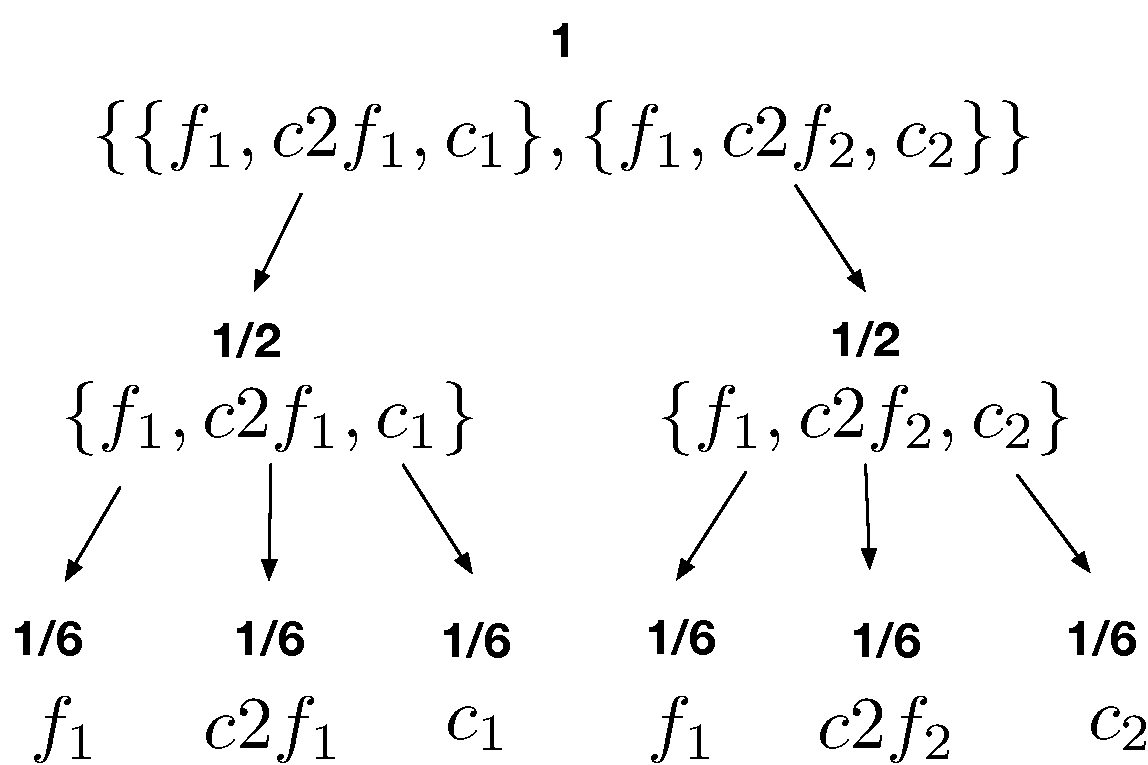
\includegraphics[width=.45\textwidth]{figures/why_distribution}
%   \caption{Distribution of credit using why-provenance-based DS for tuple $o_1$.}
%   \label{figure:why_prov_distribution}
% \end{figure}

% Figure \ref{figure:why_prov_distribution} shows the distribution of credit with why-provenance-based DS for tuple $o_1$.
% The credit is first equally divided between the two witnesses, so that both receive credit $1/2$. 
% The credit is then further divided among the tuples in each witness. Since each witness has three tuples, each tuple in a witness receives $1/6$ of credit. At the end of the distribution, $f_1$ receives a total credit of $1/3$, and the other tuples receive $1/6$ each.
% This distribution better reflects the role of $f_1$ in the generation of $o_1$ since, as discussed earlier, it is the only mandatory tuple for $o_1$ to appear in the output; only one of the two other pairs of tuples are necessary for $o_1$ to appear in the result. 

% This example illustrates that why-provenance can better reward input tuples depending on their role. Tuples that appear in more than one witness are rewarded more than others. 
% \eat{This means that tuples that are more important to the generation of the output, since they are used more by the query, are rewarded more than tuples that are ``interchangeable'' with others. }

\subsection{A How-Provenance Based Distribution Strategy}
\label{section:how_prov_distr_tuples}

%\scream{You did not talk about coefficients in section 4, you only talked about monomials.}

%How-provenance conveys more information than why-provenance since it not only captures what tuples are relevant to the output and in which combination, but also how they are used. The ``how" is captured through the provenance polynomials.

The how-provenance-based DS first distributes the credit to the monomials of the polynomial accordingly to the weight represented by their coefficients, then to the tuples of each monomial accordingly to the weights represented by their exponents. 

To define the DS more formally, we introduce some notation and illustrate it using the provenance polynomial $\mathcal{H}$ shown in Figure \ref{figure:how_example}. This notation is also shown  in Table \ref{tab:notation} for easy reference.


\begin{figure}[]
\centering
  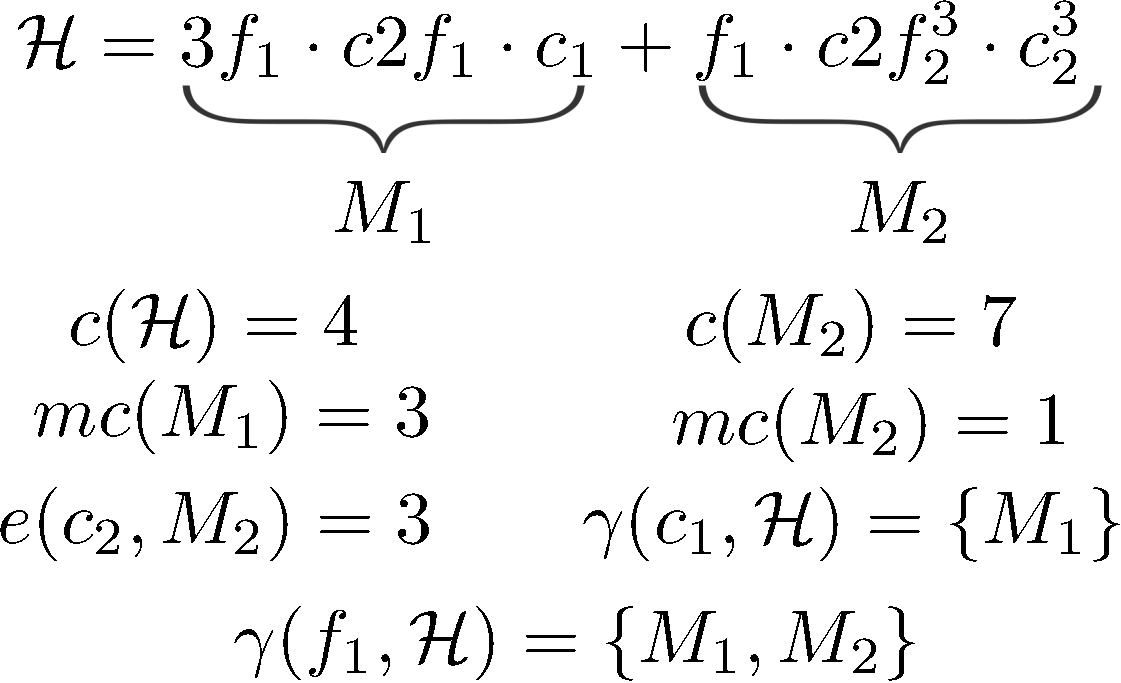
\includegraphics[width=.4\textwidth]{figures/how_example}
  \caption{Illustration of notation used to define the how-provenance based DS } %in Definition \ref{def:how_distribution}.}
  \label{figure:how_example}
\end{figure}

%In this figure we show the notation that we use to refer to different information taken from the provenance polynomial. 
We call $c$ the function that, given a polynomial, returns the sum of its coefficients; thus $c(\mathcal{H})=\;3+1=4$. 
\rone{We call $e$ the function that, given a monomial, returns the sum of its exponents, thus $e(M_2)=1+3+3=7$.}
$mc$ is the function that takes as input a monomial and returns its coefficient; thus $mc(M_1) = 3$. 
\rone{$te$ is a function that takes as input a tuple and a monomial, and returns the exponent of the tuple in the monomial, if present; thus $te(c_2, M_2)=3$}. 
Finally, $\gamma$ takes as input a tuple and the whole polynomial, and returns a set of monomials containing that tuple, if present in the polynomial; thus $\gamma(f_1, \mathcal{H})=\;\{M_1, M_2\}$, $\gamma(c_2, \mathcal{H})=\;\{M_2\}$. 

\eat{
%\scream{This needs to be simplified.  Get rid of the mathematical notation and just give an English definition.}
More formally, consider the provenance polynomial $\mathcal{H} = H(Q, I, o)$ of a tuple $o$. We define: 
\begin{enumerate}
	\item $c(\mathcal{H}) = n$ the function $c: \mathbb{N}[TupleLoc] \mapsto \mathbb{N}$ that, given a polynomial, returns the sum of its coefficients;
	\item $c(M)$ the function $c: \mathcal{M} \mapsto \mathbb{N}$ that, given a monomial $M$, returns the sum of its exponents (with $\mathcal{M} \subset \mathbb{N}[TupleLoc]$ such that $\mathcal{M}$  is made only by the monomials $M$ in $\mathbb{N}[TupleLoc]$); 
	\item $e(t, M)$ the function $e: TupleLoc \times \mathcal{M} \mapsto \mathbb{N}$ that, given in input a tagged tuple and a monomial, returns the exponent of that tuple inside the monomial;
	\item $mc(M)$ the function $mc: \mathcal{M} \mapsto \mathbb{N}$ that, given in input one monomial, returns its coefficient;
	\item $\gamma(t, \mathcal{H})$ the function $\gamma: TupleLoc \times \mathbb{N}[TupleLoc] \mapsto \mathcal{M}$ that, given a tuple $t$ and a provenance polyomial $\mathcal{H}$, returns the (possibly empty) set of monomials $M$ in $\mathcal{H}$ such that $t$ appears in $M$.
\end{enumerate}
}
%\scream{You need to give a little example to clarify the ideas.}
\begin{definition}{How-Provenance-Based Distribution Strategy}
    \label{def:how_distribution}\\
    Let $I$ be a database instance, $Q$ a query over $I$, $o \in Q(I)$ an output tuple, $\mathcal{H}$ be the provenance polynomial for $o$, and $k_o$ the credit given to $o$.
    The credit given to tuple $t$ in $I$ is:
    \[
    f_{I, Q}(t, k_o) = \frac{k_o}{c(\mathcal{H})} \sum_{M \in \gamma(t, \mathcal{H})} mc(M) \frac{\rone{te(t, M)}}{\rone{e(M)}}
    \]
\end{definition}

%We demonstrate that this is a Distribution Strategy by considering the contributions of the single monomials one at a time in the sum. With abuse of language in the following demonstration, we write $t \in M$ to indicate one tuple $t$ appearing in the monomial $M$.
%
%\[
%\begin{array}{rl}
%\sum_{t \in I}f(t, k) & = \sum_{t | \gamma(t, \mathcal{H}) = \emptyset}f(t, k) + \sum_{t | \gamma(t, \mathcal{H}) \neq \emptyset}f(t, k) \\
%    & = 0 + \sum_{M \in l(\mathcal{H})} \left(k \cdot \frac{mc(M)}{c(\mathcal{H})} \sum_{t \in M} \left[\frac{e(t, M)}{c(M)} \right]\right)\\
%    & = \frac{k}{c(\mathcal{H})}\sum_{M \in l(\mathcal{H})} \left[ \frac{mc(M)}{c(M)} \sum_{t \in M} e(t, M)  \right] \\
%    & = \frac{k}{c(\mathcal{H})} \sum_{M \in l(\mathcal{H})} mc(M)\\
%    & = k
%\end{array}
%\]

\eat{The how-provenance-based DS first distributes the credit to the monomials of the polynomial accordingly to the weight represented by their coefficients, then to the single tuples in every monomial accordingly to the weights represented by their exponents. }

Going back to the example of Table \ref{table:result_how_prov}, consider $o_1$ with provenance polynomial $f_1 c2f_1 c_1 + f_1 c2f_2 c_2$. The how-provenance-based DS firstly divides the credit between the two monomials. Since the coefficients of each monomial are $1$, the credit is split in half. If they were, for example, $1$ and $2$ respectively, $1/3$ of the credit would go to the first monomial, and $2/3$ to the second.  
Since in our example each variable has exponent $1$, the credit is further divided equally among the three variables. Thus, at the end of the computation, $f_1$ receives $1/3$, and the other tuples receive $1/6$.

% \rone{Consider instead the example where the polynomial is $f_1^2 c2f_1 c_1 + f_1^2 c2f_2 c_2$, $k_0 = 1$, and let us focus on the first monomial. It receives $1/2$ of credit, then $f_1$ receives $1/4$ of credit due to its exponent, while the other two tuples receive $1/8$.}
%If, for example, the first monomial was $f_1^2 c2f_1 c_1$, then the portion of credit of this monomial would be divided in this way: $1/2$ to $f_1$ and $1/4$ to each of the other two tuples. 


In this specific example, the how-provenance-based DS has the same outcome as the one based on why-provenance. %Consequently, one may ask if there is a significant difference between the two strategies. 
We therefore consider another query over GtoPdb, \texttt{Q2}, that asks for the families of type \texttt{gpcr} that have as contributor a researcher located in the UK:

\vspace{2mm}
{\footnotesize
\begin{adjustwidth}{25pt}{5pt}
\begin{verbatim}
	Q2: SELECT DISTINCT F.name 
	FROM family as F JOIN
		(SELECT DISTINCT f.name AS name
		FROM family AS f JOIN contributor2family AS c2f ON f.id = c2f.family_id
		JOIN contributor AS c ON c2f.contributor_id = c.id
		WHERE c.country = "UK") AS R ON F.name = R.name
	WHERE F.type = "gpcr"
\end{verbatim}	
\end{adjustwidth}
}
\vspace{2mm}

\begin{table}[]
\centering
  \begin{tabular}{|l||c|}
  \hline
    id & name\\
    \hline
    $oxs_1$ &  Dopamine Receptors\\
    \hline
  \end{tabular}
  \newline
\vspace{2mm}
  \begin{tabular}{c | c | c}
  	lineage & why-provenance & how-provenance   \\
  	$\{f_1, c2f_1, c_1, c2f_2, c_2\}$ & $\{\{f_1, c2f_1, c_1\}, \{f_1, c2f_2, c_2\}\}$ & $f_1^2 c2f_1 c_1 + f_1^2 c2f_2 c_2$\\
  \end{tabular}
    \caption{Result of query \texttt{Q2} applied on the database of Table \ref{table:running_example} and its different provenances. The reported numbers are the credit distributed through the process.}
  \label{table:difference_result}
\end{table}

The result of \texttt{Q2} is shown in Table \ref{table:difference_result}, and consists of one tuple, $oxs_1$, annotated with each of the three provenances. As can be seen, lineage and why-provenance are identical to those of the tuple $o_1$ in the previous example. 
The how-provenance, however, is different since tuple $f_1$ is used twice: first in the join of the inner query, and second in the join of the outer query. This information is lost in the first two forms of provenances since they are sets, but it is captured in how-provenance through the use of the operator `$\cdot$'.

%\scream{This polynomial still doesn't have coefficients other than 1, but ok. Why don't you rewrite the polynomial to $f_1^2c2f_1c_1 + f_1^2c2f_2c_2$ to make the exponents clearer?}

\begin{figure}[]
\centering
  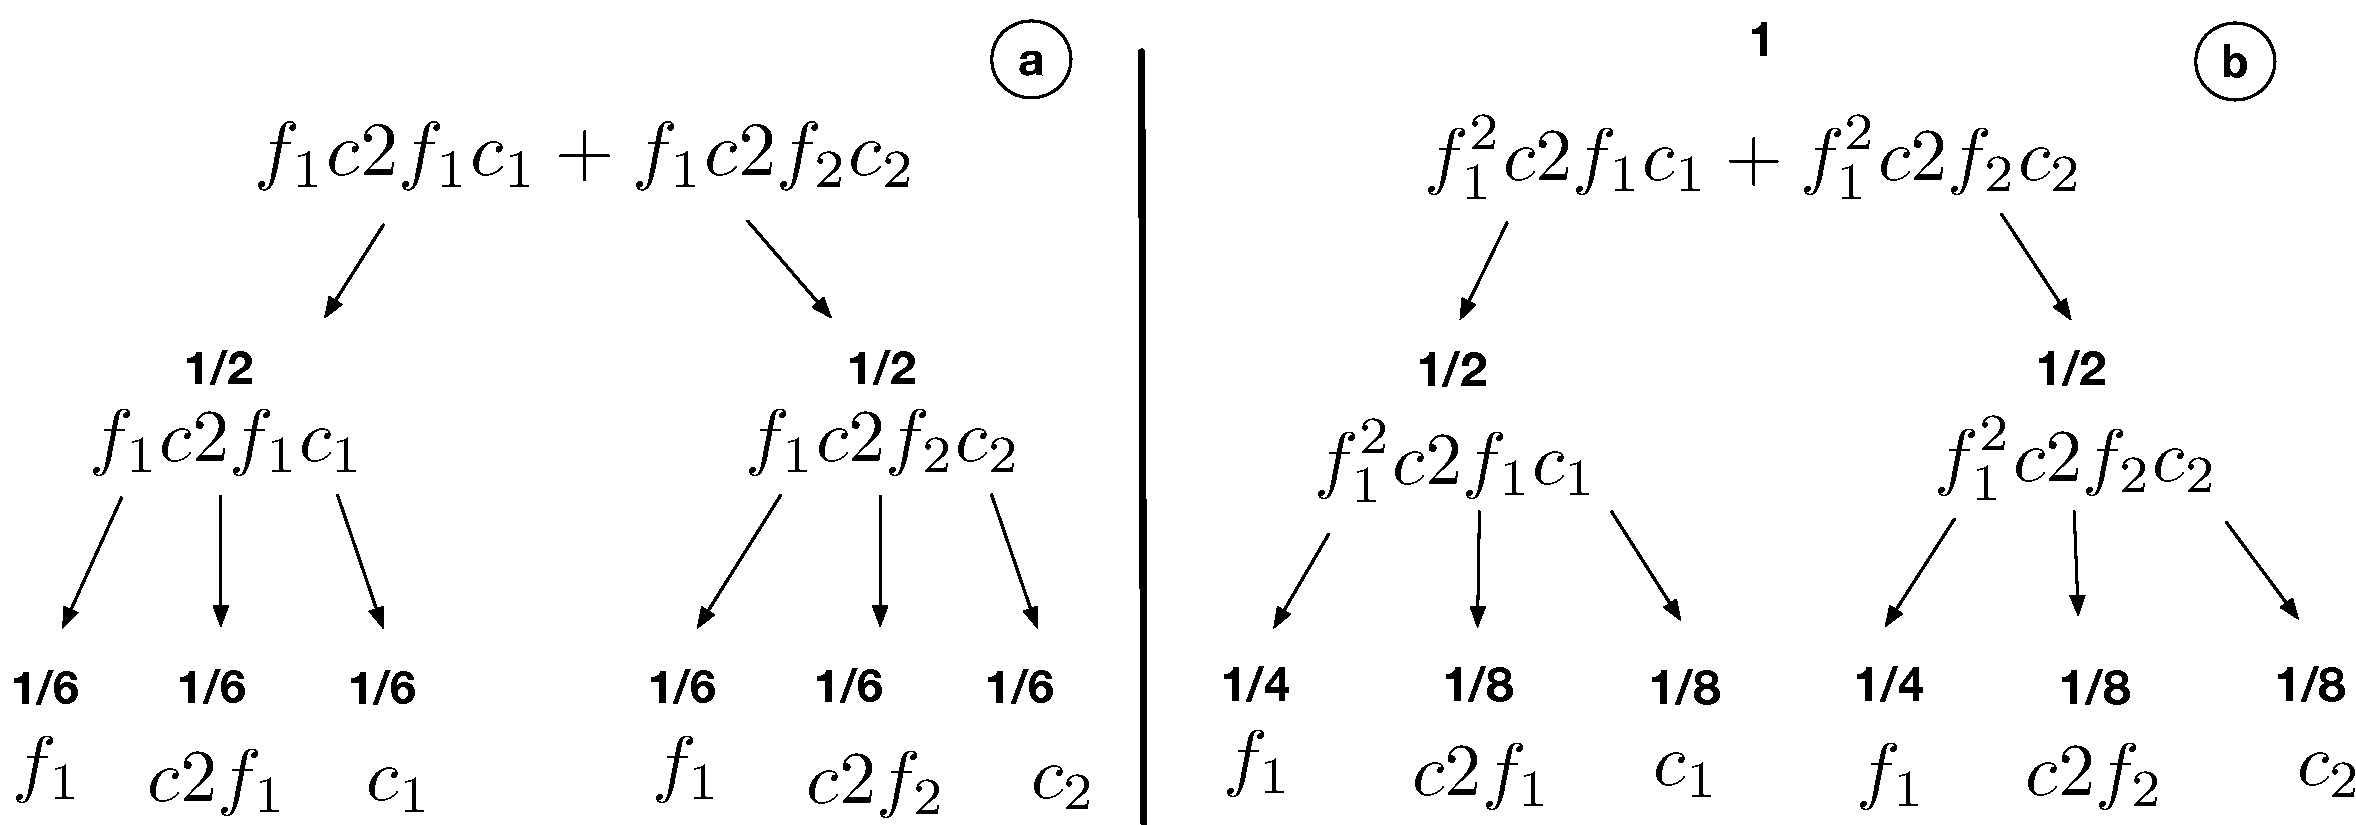
\includegraphics[width=.8\textwidth]{figures/new_comparison}
  \caption{Comparison of different distributions obtained with the how-provenance-based DS with queries \texttt{Q1} and \texttt{Q2}.}
  \label{figure:distributions_differences}
\end{figure}


Figure \ref{figure:distributions_differences} shows the differences between the three DS for the tuple $o_1$ of Table \ref{table:difference_result}. Subfigure \ref{table:difference_result}.a uses lineage, sub-figure \ref{table:difference_result}.b uses why-provenance, and sub-figure \ref{table:difference_result}.c uses how-provenance. 
The DS based on the provenance polynomial gives credit $1/2$ to $f_1$, and $1/8$ to the other tuples.
This is reasonable since \texttt{Q2} relies on $f_1$ even more than \texttt{Q1} does. 
The distribution based on how-provenance rewards $f_1$ more, showing that how-provenance is even more sensitive to the tuples' role in a query than why-provenance. %In this case, the why-provenance is not sensible to this difference. 
This is a direct consequence of the fact that, as proven in \citep{howProvenanceGreen}, how-provenance is more general than why-provenance and lineage, in the sense that it contains more information. 

\rtwo{\subsection{Responsibility-based Distribution Strategy}}
% Given the lineage of an output tuple $o$, it is first possible to compute the type of causality of each of tuple in its lineage, distinguishing between counterfactual and actual causes, by testing what happens as a result of removing single tuples and contingency sets of other tuples of the lineage.
% It is then possible to compute their responsibility through the minimal contingency sets found in this way. 

% One possible option for defining a distribution strategy using responsibility is to simply assign the responsibility of a tuple as its credit. In this way, responsibility is both a way to compute credit and to distribute it.
% Using the example of Table \ref{table:result_responsibility}, in the case of output tuple $o_1$, $f_1$ receives credit 1 and the other tuples receive credit $0.5$. 

As described in Section \ref{sec:responsibility}, causality and responsibility is 
new information that is added to lineage.   One possible option for defining a distribution strategy using responsibility is to simply assign the responsibility of each tuple in the lineage of an output tuple as its credit. In this way, responsibility is both a way to compute credit and to distribute it.
Using the example of Table \ref{table:result_responsibility}, in the case of output tuple $o_1$, $f_1$ receives credit 1 and the other tuples receive credit 0.5.


However, we want a DS that is also a function of the input credit value $k$ in order to be comparable with the other three strategies proposed so far.
We define a new DS based on responsibility that is a function of the quantity of credit $k_o$ that assigns to each tuple of the lineage a portion of this credit weighted by its normalized quantity of responsibility.
This will give a bigger portion of credit to tuples that are higher in the responsibility ranking.
Formally:
\newline
\begin{definition}{Responsibility-based Distribution Strategy}\\
\label{def:resp_ds}
Let $I$ be a database instance, $Q$ a query over $I$, $o \in Q(I)$ an output tuple, $L$ the lineage of $o$, and $k_o$ the credit given to $o$. The credit given to tuple $t$ in $I$ is:
\[
	f_{I, Q}(t, k_o) = k_o \frac{\rho_t}{\sum_{t' \in L} \rho_{t'}}
\]
where $\rho_j$ is the responsibility of tuple $j$ as in Definition \ref{def:responsibility}.
\end{definition}


\begin{figure}[]
\centering
  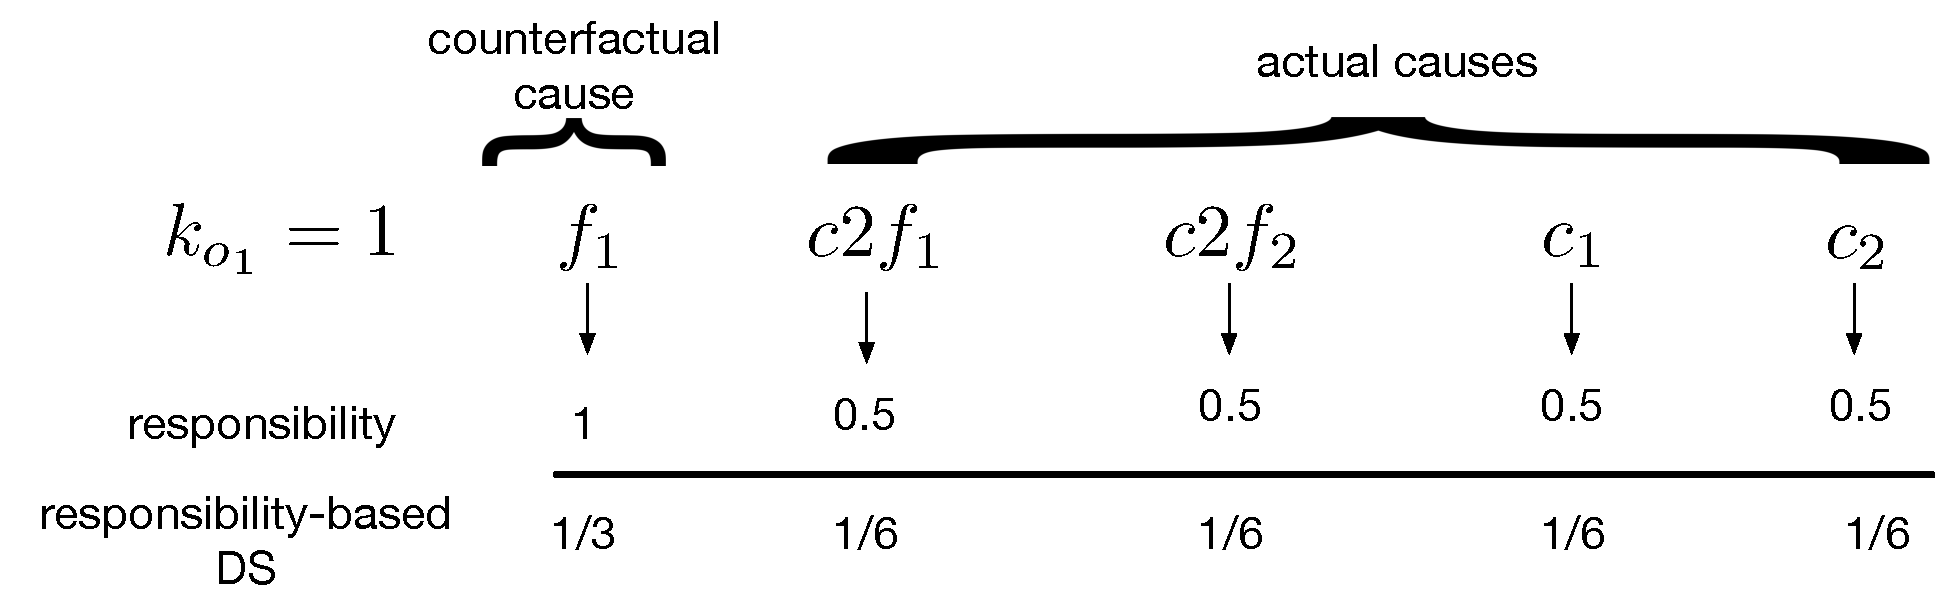
\includegraphics[width=.7\textwidth]{resp_example}
  \caption{Example of distribution of credit using 
%  responsibility and normalized responsibility and 
    the responsibility-based DS, assuming $k_o = 1$.}
  \label{fig:resp_example}
\end{figure}

Note that only the tuples that belong to the lineage will receive a quantity of credit $> 0$. Furthermore, the more important the tuple is, i.e., the higher its responsibility, the larger the quantity of credit received. 

Figure \ref{fig:resp_example} shows the responsibility and credit assigned to the tuples of the lineage of the output tuple $o_1$ of Table \ref{table:result_responsibility}. 
Assuming that $k_{o_1} = 1$, $f_1$ receives credit $1/3$, while the others receive credit $1/6$. 
As we see, the DS in this case returns the same distribution as that obtained using why-provenance as shown in Figure \ref{figure:distributions_differences}.
This is not always the case though, as we show in the example of Section \ref{sec:synth_queries}.

\rtwo{\subsection{Shapley value-based Distribution Strategy}}

As with responsibility, the Shapley value can be seen both as a method to generate and distribute credit. Moreover, it can be seen that, using the definition of Shapley value for Boolean queries given in Section \ref{sec:shapley_value}, the sum of the Shapley values of all the tuples of the lineage $L$ of an output tuple $o$ is $1$. Thus, the definition of a Shapley value-based distribution strategy is straightforward:

\begin{definition}{Shapley Value-Based Distribution Strategy} \\
	Let $I$ be a database instance, $Q$ a query over $I$, $o \in Q(I)$ an output tuple, and $k_o$ the credit given to $o$. The credit given to tuple $t$ in $I$ is:
	\[
		f_{I, Q}(t, k_o) = k_o \cdot 
		Shapley(\bar{Q}_o, I, t)
	\] 
	where $\bar{Q}_o$ is the Boolean query such that, given the set of facts $D$, $\bar{Q}_o(D) = 1$ if and only if $o$ is in the output of $Q$ on $D$.
\end{definition}

As shown in Table \ref{table:result_shapley}, tuple $f_1$ in $o_1$'s lineage takes credit $7/15$ when $k_{o_1} = 1$, while the other tuples of the lineage take credit $2/15$. This DS still rewards $f_1$ more than the other tuples, since it is more important than the other tuples of the lineage. This DS thus behaves differently from all the other four previous strategies. In particular, $f_1$ is rewarded more with this DS than with the others.

In the case of $o_2$ there is only one witness set, thus this DS behaves like all the others, distributing $1/3$ of credit to each tuple in the lineage. 

\section{Experimental Evaluation}
\label{sec:experiments}
To understand the trade-offs between these Distribution Strategies (DSs), we perform four sets of experiments using queries over target families presented on the GtoPdb website. The first set of experiments use real queries extracted from citations to GtoPdb published in the British Journal of Pharmacology.  
The second set uses synthetically produced provenance polynomials, corresponding to more complex queries, in order to better highlight the differences between the DSs.
The third set of experiments considers the accrual of credit over time by the three strategies, again using synthetic queries.
The fourth set of experiments shows how the DSs compare to traditional citations in giving credit to data curators using both real and synthetic queries.
%We close by discussing the relative execution times of the three strategies.

%All experiments were carried out on a MacBook Pro %13-inch, 2019 
%with a 2.4 GHz processor Intel Core i5 quad-core and 8 GB of memory at 2133 MHz.  
The source code for the experiments is written in Java and supported by a PostgreSQL database. For purposes of reproducibility, the code we used for our experiments and all queries are available here: \url{https://bitbucket.org/dennis_dosso/credit_distribution_project}.

\subsection{Real-world queries}
\label{sec:real_world_queries}

\begin{figure}[t]
\centering
  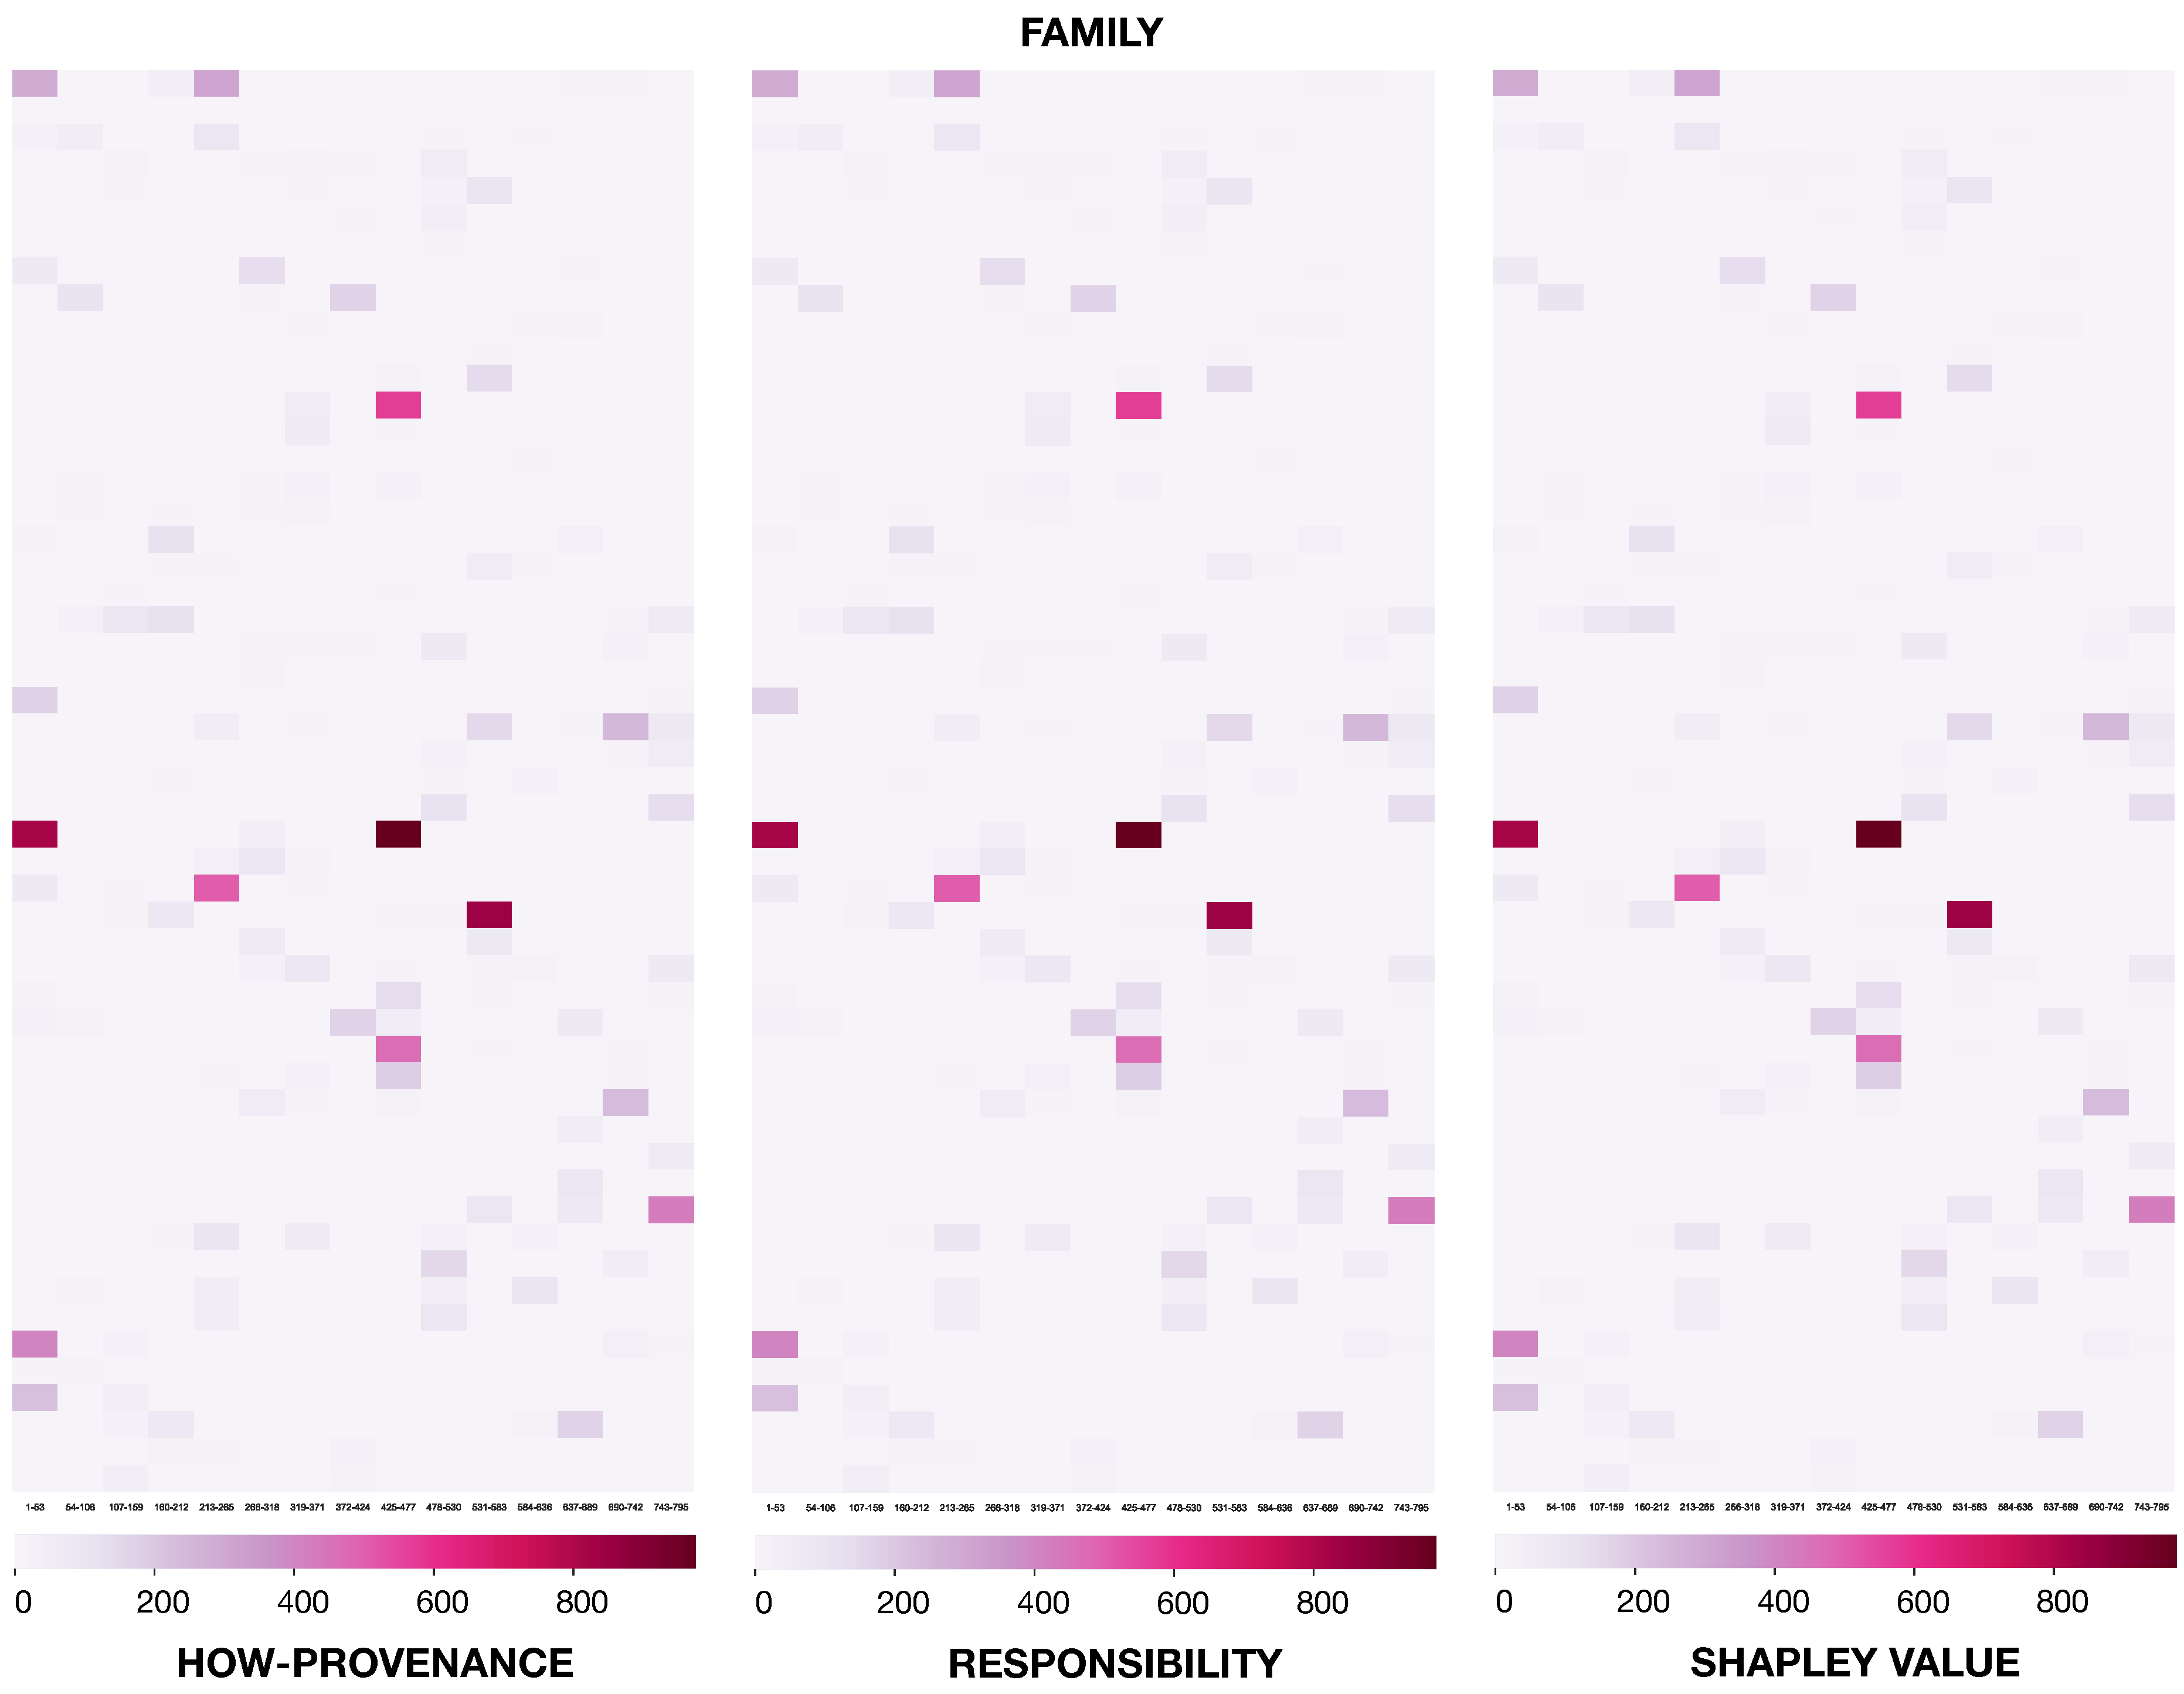
\includegraphics[width=\textwidth]{paper_based}
  \caption{Comparison of four DS on the same table \texttt{family} using the distribution given by the queries retrieved from papers. Each cell is a tuple.}
  \label{figure:comparison_on_papers}
\end{figure}


%We evaluate the proposed distribution strategies on GtoPdb, and in particular, we focus on target families described on the GtoPdb website. 

%When a paper uses data from GtoPdb, it can cite the full database, a webpage of interest, or a subset of data extracted with a query. 

Examples of real queries are drawn from papers published in the British Journal of Pharmacology (BJP)~\footnote{\url{https://bpspubs.onlinelibrary.wiley.com}}.  Each time a paper in this journal cites a webpage from GtoPdb, it reports the URL of the page. From this URL, the query used to obtain the webpage data can be determined. 
We considered all $889$ papers in BJCP citing the IUPHAR/BPS Guide to pharmacology \citep{iuphar2018} as of October 2020, and extracted all webpage URLs to GtoPdb contained within the paper.\footnote{The IUPHAR/BPS Guide is a journal that describes the structure and evolution of GtoPdb. At the time of writing, it had received more than $1200$ citations on Google Scholar.}

\eat{
There are eight target family webpages linked from the GtoPdb website: \emph{GPCR}, \emph{Ion channels}, \emph{NHRs}, \emph{Kinases}, \emph{Catalytic receptors}, \emph{Transporters}, \emph{Enzymes} and \emph{Other protein targets}.}
The queries that we inferred are those used to build target family webpages within GtoPdb.
An example was given in Figure \ref{figure:family_structure}, where we show how the structure of the ``Adenosine receptors'' family can be mapped into  queries over the underlying database. %to get the information reported in the corresponding webpage. 
In GtoPdb, all target family pages share a similar structure; the only difference is that individual sections, such as ``contributors'' or ``further readings'', may be missing.
Therefore, the same queries can be used to build all of the target family pages by changing the family id used in the query (for example, in Figure \ref{figure:family_structure}, it is 3).
Note that the queries are fairly simple SQL queries, and fall into a class called ``select-project-join" or ``SPJ" queries. 
A total of more than $12K$ different queries were built in this way.
Without loss of generality, we give each tuple in the output of a query a credit of $1$.

\paragraph{Results} Figure \ref{figure:comparison_on_papers} shows the heat-maps obtained by the distribution of credit according to the \rtwo{five} DS on one of the tables in the underlying database, \texttt{family}, 
%describes the characteristics and necessary information of the receptor families and, as can be seen in Figure \ref{figure:family_structure}, it 
which is often joined with other tables in the database to build the webpages. Each cell in a heat-map represents a tuple of the \texttt{family} table and the color indicates the amount of credit attributed to such tuple.
It can be seen that the result of  credit distribution over \texttt{family} is the same for all \rtwo{five} strategies. The same result is also obtained with the other tables of the database used by the queries shown in Figure \ref{figure:family_structure}. 

The reason why credit distribution is the same for all \rtwo{five} strategies is that the queries are all simple SPJ queries, which use each table only once and do joins on key attributes. 
Under these conditions, each tuple of the output presents: (i) a how-provenance that is a single monomial with coefficient one and exponent one in each variable; (ii) a why-provenance with only one witness; (iii) a lineage that is the same of the witness in the basis, \rtwo{(iv) all tuples are counterfactual causes when considering responsibility, and (v) all tuple have the same importance in the production of the output tuples according to their Shapley value}.
Hence, for these queries, the \rtwo{five} DSs behave in the same way: credit is uniformly distributed among the tuples of the lineage. 

To illustrate this, consider one of the queries in Figure \ref{figure:family_structure} which is used to build the output webpage:

\vspace{2mm}
{\footnotesize
\begin{adjustwidth}{25pt}{5pt}
	\begin{verbatim}
	Q3: SELECT c.first_names, c.surname
	FROM contributor2family AS cf JOIN contributor AS c ON 
	cf.contributor_id = c.contributor_id 
	WHERE f.family_id = 3
\end{verbatim}
\end{adjustwidth}
}
\vspace{2mm}

\texttt{Q3} returned $10$ tuples from the version of GtoPdb used. 
The first tuple, \texttt{<Bertil B., Fredholm>}, has  $c_{939} \cdot c2f_{496}$ as its provenance polynomial.
$c_{939}$ represents the provenance token of a tuple in \texttt{contributor}, and $c2f_{496}$ the provenance token of a tuple in table \texttt{contributor2family}. 
The why-provenance of this tuple is $\{\{c_{939}, cf_{496} \}\}$, its lineage is $\{c_{939}, c2f_{496} \}$, \rtwo{both these tuples are counterfactual causes and have a responsibility of one.}
Therefore, the credit assigned to these tuples is $1/2$ using all five DS.
This happens for all the tuples in the output of each query of GtoPdb, thus making the distributions equivalent over all outputs.

However, this is not the case with more complex queries. As we showed in the previous section, when two or more tuples are merged as a result of a projection or union, the credit distributions will differ between the strategies. %These are represented as multiple witnesses and multiple monomials. 

\begin{comment}
	
To give an example of how the CDS can differ from one another in their behavior, let us consider a different query:

\vspace{2mm}
{\footnotesize
\begin{adjustwidth}{25pt}{5pt}
	\begin{verbatim}
	Q4: SELECT f.name AS name
	FROM family AS F JOIN
	(SELECT DISTINCT f.family_id, f.name
	FROM "family" AS f JOIN contributor2family AS cf ON 
	f.family_id = cf.family_id 
	JOIN contributor c ON 
	cf.contributor_id = c.contributor_id 
	WHERE c.country = 'UK') AS R 
	ON F.name = R.name
\end{verbatim}
\end{adjustwidth}
}
\vspace{2mm}

Here the innermost query retrieves all the names and ids of the families written by an author from the UK producing a relation called $R$. This relation is then joined with the table \texttt{family} on the attribute \texttt{name}. 

One output tuple of this query is \texttt{<Histamine receptors>}, that has the following provenance polynomial:

{\footnotesize
\[
\begin{array}{c}
	f_{625}(f_{625} c2f_{656} c_{184} + f_{625} c2f_{113} c_{180} + f_{625} c2f_{283} c_{198} +\\ 
	+ f_{625} c2f_{550} c_{865} + f_{625} c2f_{573} c_{101} + f_{625} c2f_{95} c_{109} )
\end{array}
\]
}

As already discussed, the different monomials represent possible \emph{alternatives} of combinations of tuples that produce the considered output tuple. 
Tuple $f_{625}$ is used multiple times with different joins, thus it appears in each monomial. 
The last join, performed in the outmost query, is responsible for the final multiplication of $f_{625}$ with the rest of the polynomial between parenthesis.

From this polynomial we compute the why-provenance as a set of six different witnesses:

{\footnotesize
\[
\begin{array}{c}
\{\{ f_{625}, c2f_{656}, c_{184} \}, \{ f_{625}, c2f_{113}, c_{180} \} 
\{ f_{625}, c2f_{283}, c_{198} \}, \\ \{ f_{625}, c2f_{550}, c_{865} \},
 \{ f_{625}, c2f_{573}, c_{101}\} , \{f_{625}, c2f_{95}, c_{109} \}\}	\\
\end{array}
\]
}

And corresponding lineage:
{\footnotesize
\[
\begin{array}{c}
	\{ f_{625}, c2f_{656}, c_{184}, c2f_{113}, c_{180}, 
  c2f_{283}, c_{198}, c2f_{550}, c_{865}, 
  c2f_{573}, c_{101}, c2f_{95}, c_{109}\}
\end{array}
\]
}

\begin{figure}[tb]
  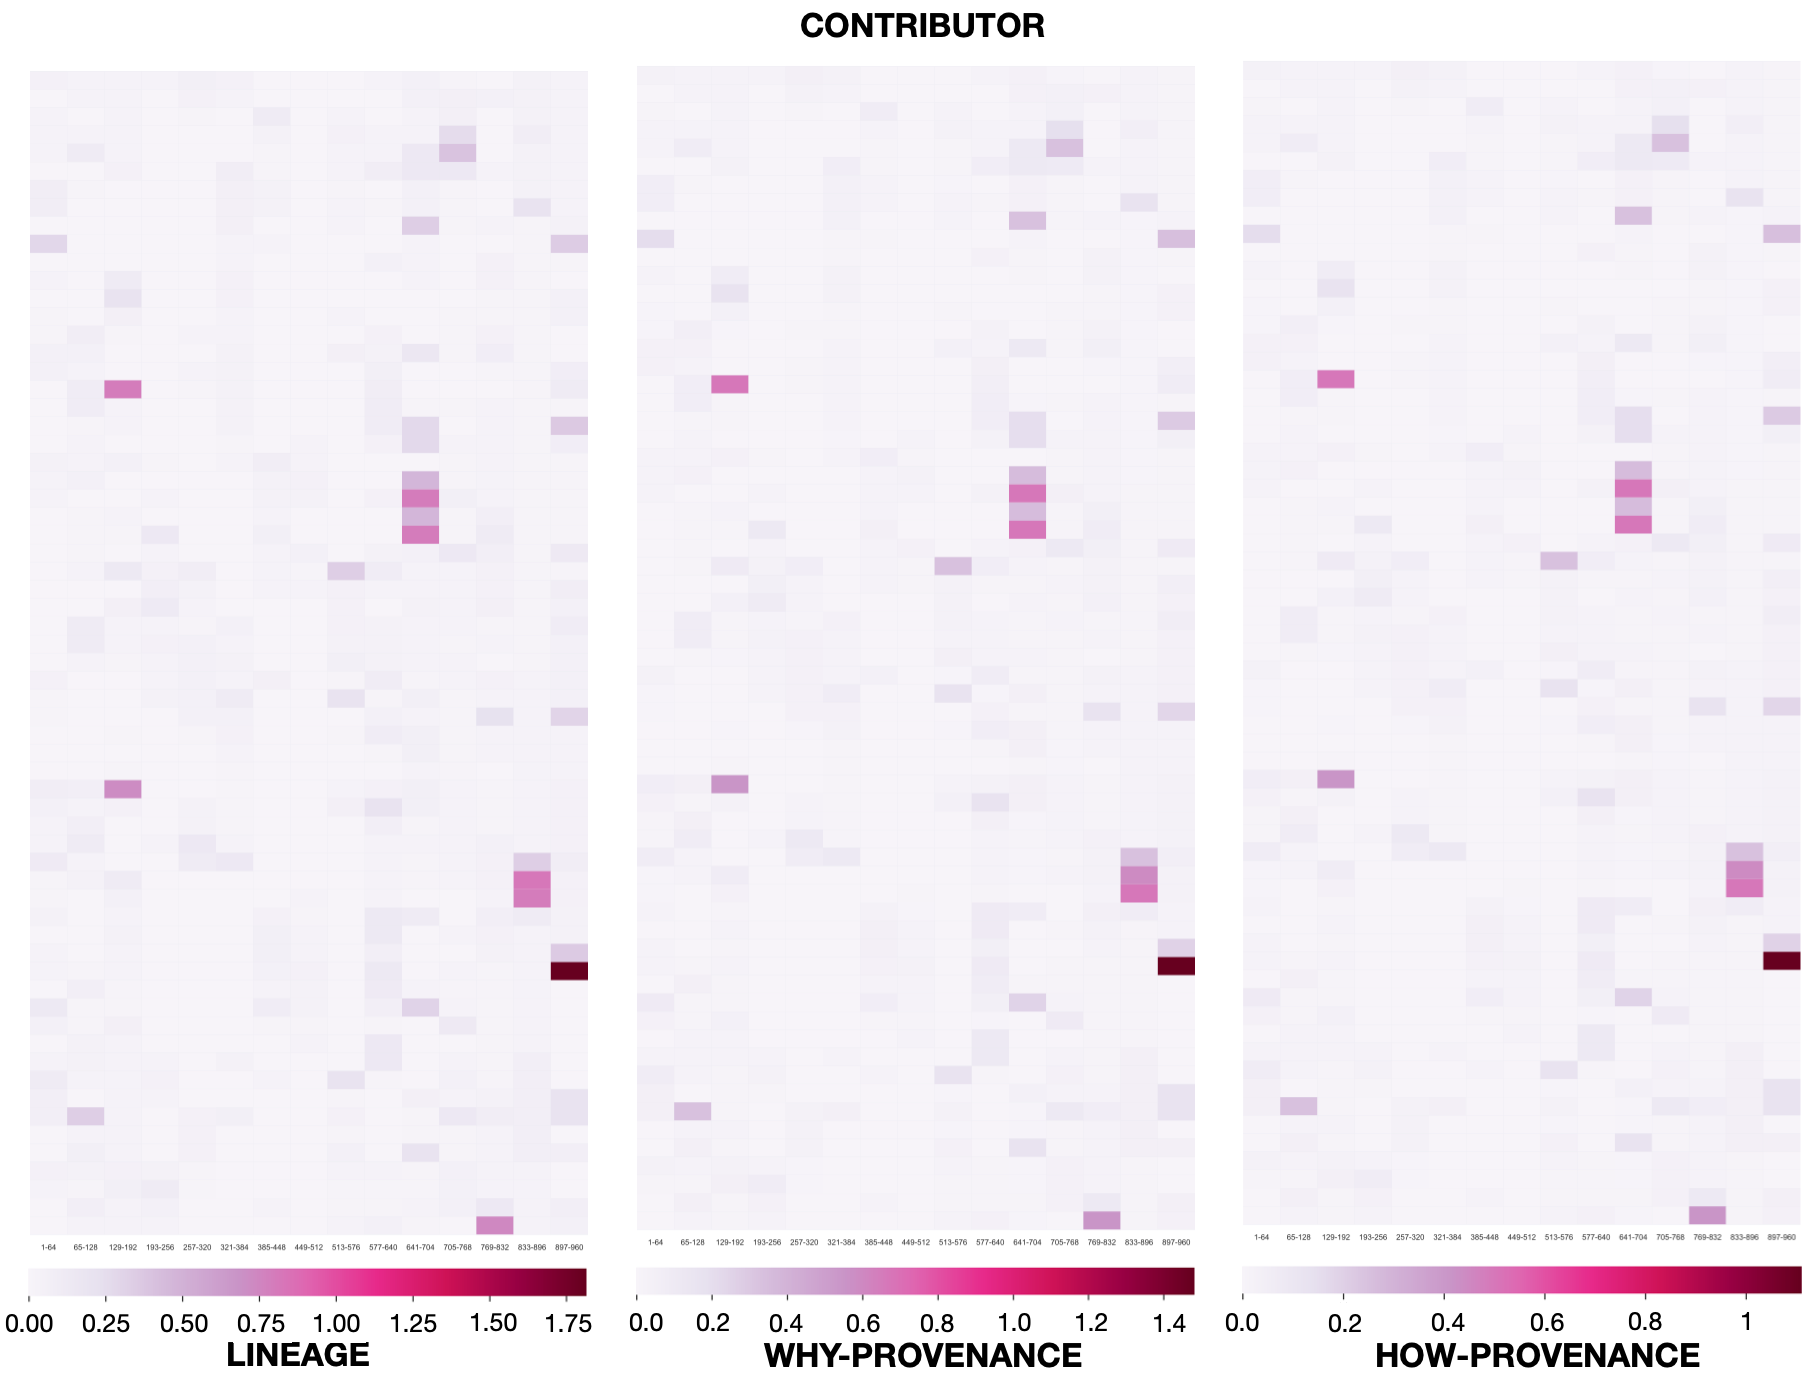
\includegraphics[width=1\textwidth]{figures/synthetic_queries}
  \caption{Comparison of three DS on the same table \texttt{family} after the distribution of the credit connected to query \texttt{Q4}.}
  \label{figure:comparison_on_synthetic_query_1}
\end{figure}

This was only one tuple among the $86$ obtained from this query. If we assign credit $1$ to all these tuples and distribute it with the different strategies, we obtain the result shown in Figure \ref{figure:comparison_on_synthetic_query_1} for the table \texttt{contributor}.
At first sight, it may appear that the three distributions produce the same result. This is only partially true: the heat maps appear equal, but the absolute values assigned to each tuple are different. 
This is more evident if we look at the legend of each heat-map, where the maximum quantity of credit is different for each distribution. The one performed through lineage is around $1.8$, the why-provenance's one is around $1.4$, and the one based on how-provenance is around $1.1$. 

To understand what is happening with this query in this specific table, consider the output tuple \texttt{<Histamine receptors>} and its provenances, as discussed above.
Let us focus on its lineage. There are a total of six authors for this family and $13$ tuples in total in the lineage. 
Thus, using the lineage-based DS, each tuple belonging to the \texttt{contributor} table (i.e. $c_{184}, c_{180}, c_{198}, c_{865}, c_{101}, c_{109}$) receives credit equal to $1/13$.
Tuple $f_{625}$ too receives a portion of credit equal to $1/13$.

Let us consider now why-provenance. Tuple $f_{625}$ appears six times in six different witnesses composed of $3$ elements each. From each witness it receives a portion of credit equal to $1/18$, thus its total credit is $1/3$.
On the other hand, all the authors appear only once in each witness, thus each of them receives credit $1/18$. 
In this case, why-provenance is recognizing more credit to tuple $f_{625}$, since it appears in each witness. The consequence is that this distribution is equally \emph{subtracting} credit from the other tuples in the witnesses and giving it to $f_{625}$. 
In Figure \ref{figure:comparison_on_synthetic_query_1} we are only looking at table \texttt{contributor}. 
This same effect is reproduced for each tuple of the output of query \texttt{Q4}, thus the \emph{absolute} credit values on the tuples vary depending on the deployed strategy. 
What happens is that the tuples in table \texttt{contributor} receive less credit than the one received using lineage, but in the same proportions. The heat map appears thus equal to the one obtained with lineage.
This same effect is also present with the how-provenance-based CDS. In this case, tuple $f_{625}$ is rewarded even more, since it appears with an exponent 2 in each monomial, thus attracting even more credit. 

This is also why when we look at the legend for each part of Figure \ref{figure:comparison_on_synthetic_query_1}, the maximum value reached with the lineage-based DS is higher than the one reached with the why-provenance-based DS, which in turn is higher than the one obtained with the how-provenance. This is because the different strategies reward less and less the tuples of table \texttt{contributor} and more the ones in table \texttt{family}. 

This clearly shows the ability of the different strategies to adapt to situations. All three of them can highlight the relevant tuples in the table. However, they differ in the way they reward the tuples. 
Depending on the task, one provenance can be preferred to the other. 
If the only interest is to highlight the relevant tuples, lineage is sufficient. 
If the interest is also to reward more the tuples that are fundamental to the output, one can also choose why- or how-provenance, knowing that how-provenance rewards even more than why-provenance the relevant tuples that are indispensable for the output.  

\end{comment}


\subsection{Synthetic queries}
\label{sec:synth_queries}
\eat{
let us consider the case reported in Figure \ref{figure:comparison_on_synthetic_polynomials_2}. 
The figure reports a distribution of credit performed on the table \texttt{family} through the generation of 10K \emph{synthetic} polynomials. 
We randomly generated provenance polynomials that might be the how-provenance of randomly generated synthetic queries, using the three GtoPdb tables \texttt{family}, \texttt{contributor2family}, and \texttt{contributor}. 
An example of a synthetic polynomial that will be used throughout this subsection is:
}

To see what happens with more complex queries, 
%highlight the differences between the three DS, 
\rone{we synthetically generated provenance polynomials in which the coefficients and exponents could be greater than one, and picked them at random from a uniform distribution.}
%that might be the how-provenance of randomly generated synthetic queries, 
The queries involve three GtoPdb tables: \texttt{family}, \texttt{contributor2family}, and \texttt{contributor}. 
\rone{The polynomials were generated as follows: first, the number of monomials was decided by  randomly choosing a number between one and six.  Then, we randomly chose a tuple from the  \texttt{family} table, one from the \texttt{contributor2family} table and one from the \texttt{contributor} table; these are the variables of the monomial. We then chose a coefficient for the monomial (between one and three) and an exponent for each tuple (between one and four). For the next monomial, we decided if we wanted to keep the same tuple from the table family as first tuple of the new monomial. To do so, we generated a random float number between zero and one. If the number was above $0.2$, we changed the family tuple.}

An example can be found in Figure~\ref{fig:syntheticDistributions}, which shows a sample synthetic provenance polynomial (the how-provenance), the corresponding why-provenance, lineage, \rtwo{the causality of the tuples of the lineage, together with their responsibility, and, finally, the Shapley values of the lineage tuples}.  The resulting credit distribution for each DS is also shown.

\begin{figure}
{\footnotesize{\bf How-provenance:}
$
3 f_1^3 c2f_1^2 c_1^2 + 2 f_1 c2f_2^3 c_2^3 + 4 f_5 c2f_{17}^4 c_{18}^3
$ }\\
\hspace{0.5in} 
{\footnotesize{\bf Credit distribution:}\\ $f_1 = \frac{59}{315}, f_5 = \frac{1}{18}, c2f_1 = \frac{2}{21}, c2f_2 = \frac{2}{15}, 
c2f_{17}=\frac{2}{9} , c_1 = \frac{2}{21}, c_2 = \frac{2}{15}, c_{18} = \frac{1}{6} 
$
}
\\
\\
{\footnotesize{\bf Why-provenance:}
$
\{ \{f_1, c2f_1, c_1\}, \{f_1, c2f_2, c_2\}, \{ f_5, c2f_{17}, c_{18}\} \}
$ 
}
\\
{\footnotesize{\bf Credit distribution:}\\
$
f_1 = \frac{2}{9}, f_5 = \frac{1}{9}, c2f_1 = \frac{1}{9}, c2f_2 = \frac{1}{9}, 
c2f_{17}=\frac{1}{9} , c_1 = \frac{1}{9}, c_2 = \frac{1}{9}, c_{18} = \frac{1}{9} 
$
}
\\
\\
{\footnotesize{\bf Lineage: }
$
\{f_1, f_5, c2f_1, c2f_2, c2f_{17}, c_1, c_2, c_{18} \}
$}
\\
{\footnotesize{\bf Credit distribution:}\\
$
f_1 = \frac{1}{8}, f_5 = \frac{1}{8}, c2f_1 = \frac{1}{8}, c2f_2 = \frac{1}{8}, 
c2f_{17}=\frac{1}{8} , c_1 = \frac{1}{8}, c_2 = \frac{1}{8}, c_{18} = \frac{1}{8} 
$}
\\
\\
{\footnotesize{\bf \rtwo{Causality:}}
\rtwo{counterfactual causes: $\emptyset$,\\
actual causes: $\{f_1, f_5, c2f_1, c2f_2, c2f_{17}, c_1, c_2, c_{18} \}$} \\
\rtwo{\textbf{Responsibility:}\\ 
$
f_1 = \frac{1}{2}, f_5 = \frac{1}{2}, c2f_1 = \frac{1}{3}, c2f_2 = \frac{1}{3}, 
c2f_{17}=\frac{1}{2} , c_1 = \frac{1}{3}, c_2 = \frac{1}{3}, c_{18} = \frac{1}{2}  
$
}}
\\
\rtwo{{\footnotesize{\bf Credit distribution:}\\
$
f_1 = \frac{3}{20}, f_5 = \frac{3}{20}, c2f_1 = \frac{1}{10}, c2f_2 = \frac{1}{10}, 
c2f_{17}=\frac{3}{20} , c_1 = \frac{1}{10}, c_2 = \frac{1}{10}, c_{18} = \frac{3}{20}  
$
}}
\\
\\
\rtwo{{\footnotesize{\bf Shapley value:}\\
$
f_1 = 0.258\bar{3}, f_5 = \frac{1}{8}, c2f_1 = 0.091\bar{6}, c2f_2 = 0.091\bar{6}, 
c2f_{17}=\frac{1}{8} , c_1 = 0.091\bar{6}, c_2 = 0.091\bar{6}, c_{18} = \frac{1}{8}  
$
}}

\caption{\rtwo{Sample synthetic provenance polynomial (how-provenance) and corresponding why-provenance, lineage, responsibility, and Shapley values, together with the corresponding credit distributions. The sum of Shapley values  is equivalent to the quantity of credit being distributed (assuming that the input credit is equal to $1$).}}
 \label{fig:syntheticDistributions}
 \end{figure}

\begin{figure}[tb]
  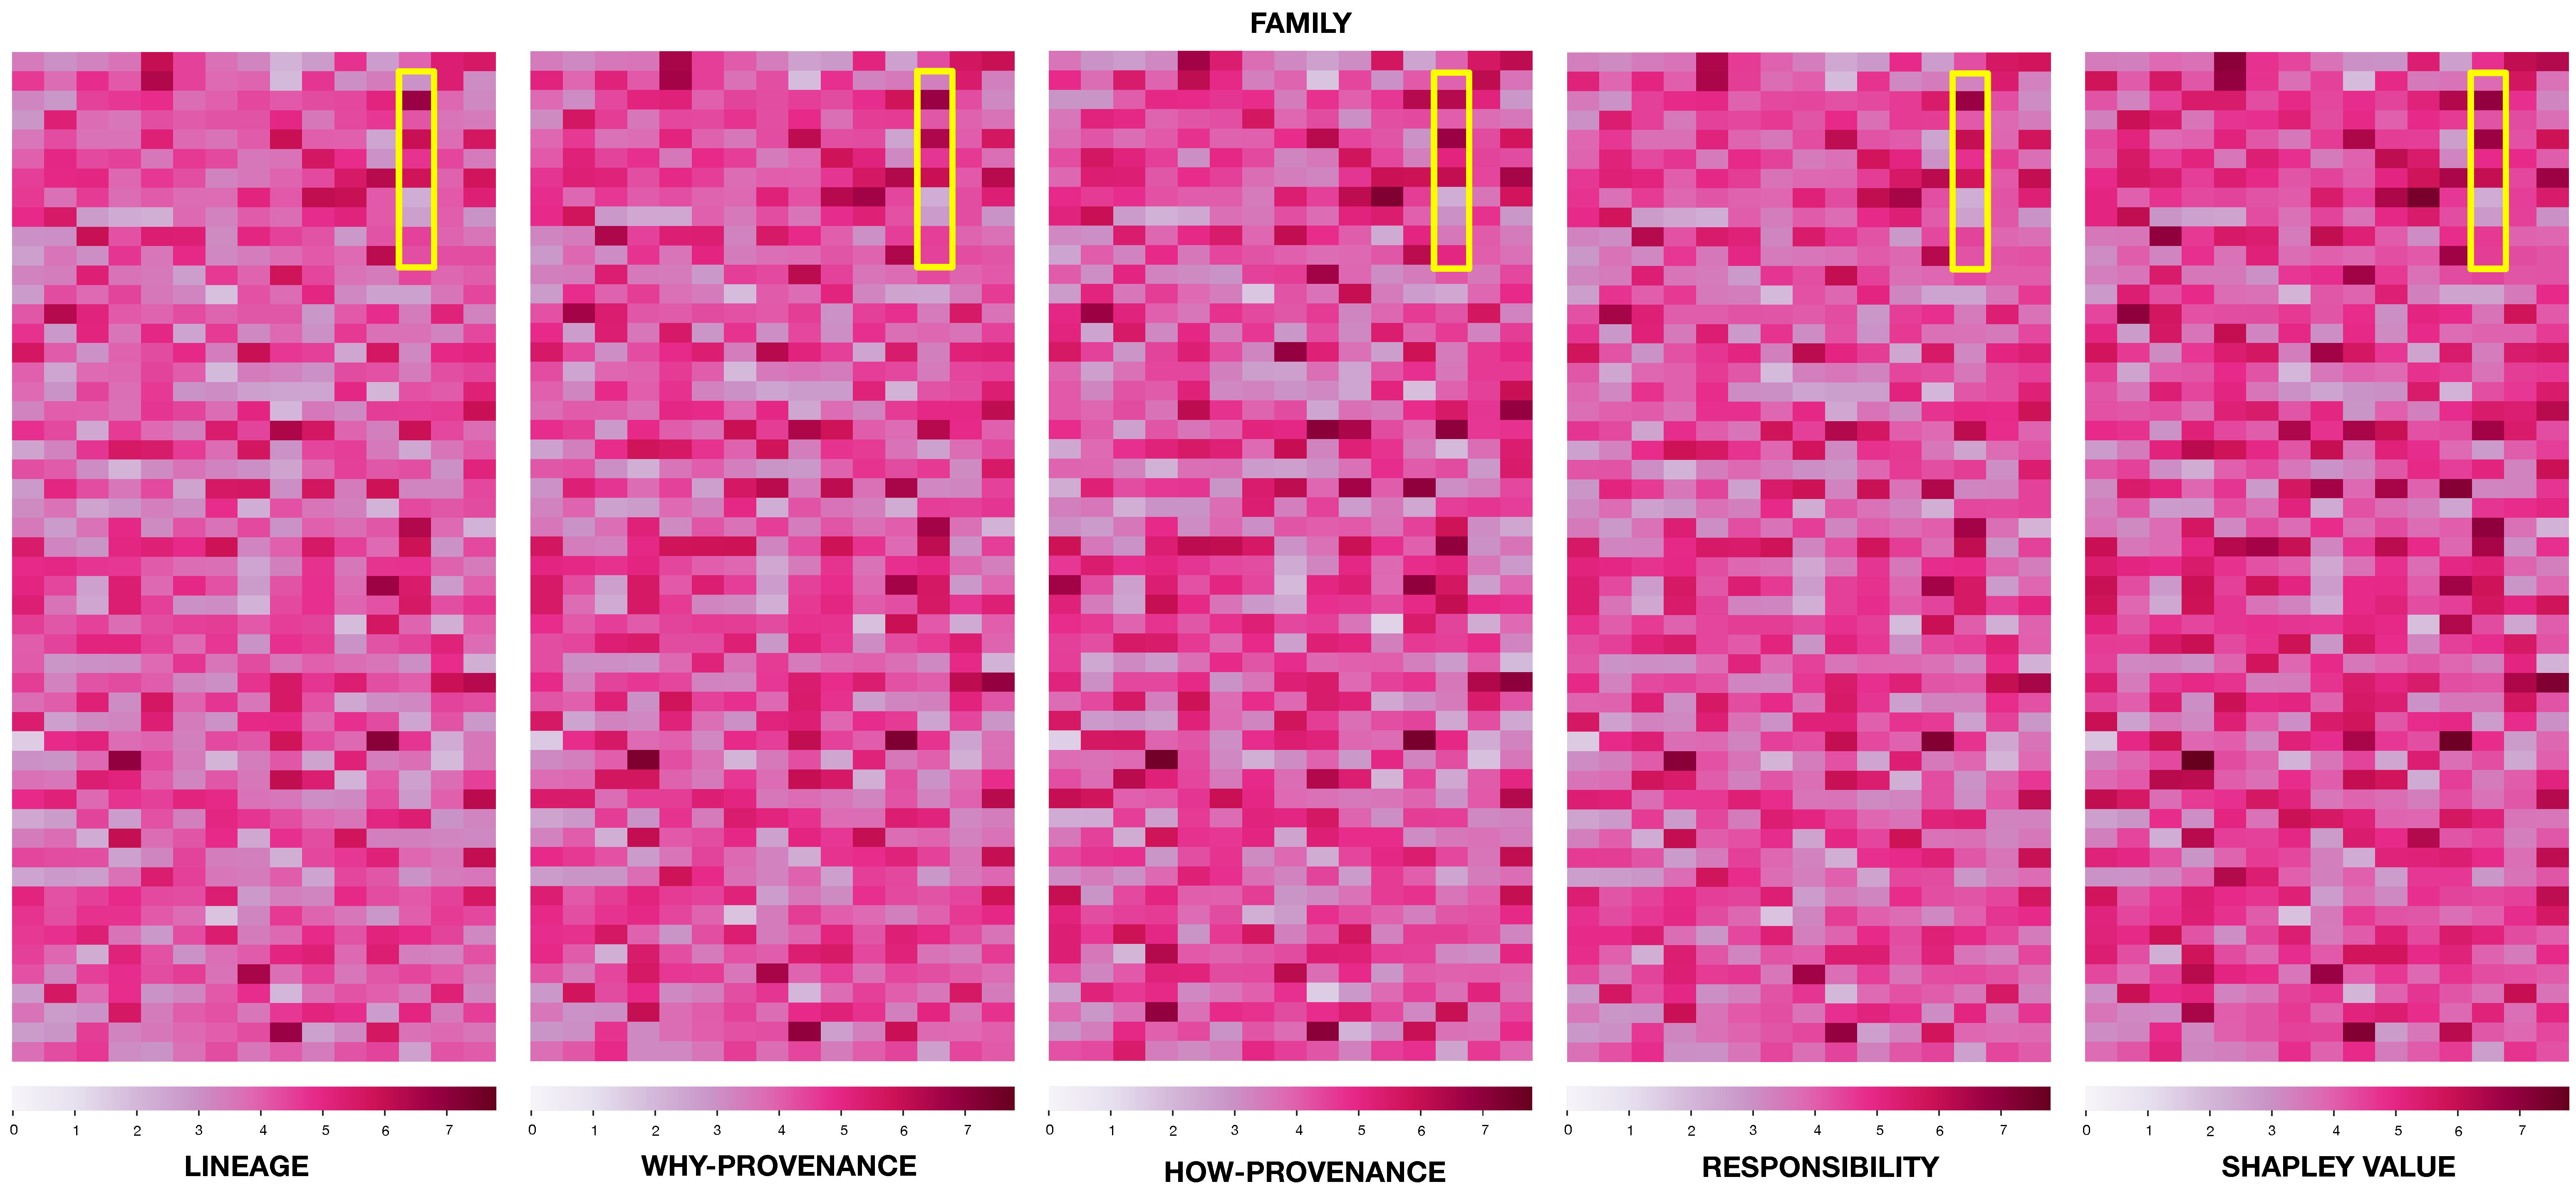
\includegraphics[width=1\textwidth]{synthetic_comparison}
  \caption{Comparison of three DS on the same table \texttt{family} after the distribution computed using 10K synthetic and randomly generated provenance polynomials. The tuples in the blue rectangles are used as example in the discussion connected to Figure \ref{fig:comparison}.}
  \label{figure:comparison_on_synthetic_polynomials_2}
\end{figure}

\eat{
An example of such a synthetic provenance polynomial is:

{\footnotesize
\[
3 f_1^3 c2f_1^2 c_1^2 + 2 f_1 c2f_2^3 c_2^3 + 4 f_5 c2f_{17}^4 c_{18}^3
\] }
The corresponding why-provenance is: 
{\footnotesize
\[
\{ \{f_1, c2f_1, c_1\}, \{f_1, c2f_2, cf_2\}, \{ f_5, c2f_{17}, c_{18}\} \}
\] 
}
and corresponding lineage is: 

{\footnotesize
\[
\{f_1, f_5, c2f_1, c_1, c2f_1, c2f_2, c2f_{17}, c_1, c_2, c_{18} \}
\]}
 
 Using {\em how-provenance}, the distribution obtained from this sample polynomial is:

{\footnotesize
\[
f_1 = \frac{59}{315}, f_5 = \frac{1}{18}, c2f_1 = \frac{2}{21}, c2f_2 = \frac{2}{15}, 
c2f_{17}=\frac{2}{9} , c_1 = \frac{2}{21}, c_2 = \frac{2}{15}, c_{17} = \frac{1}{6} 
\]
}

Using {\em why-provenance}, the distribution is:

{\footnotesize
\[
f_1 = \frac{2}{9}, f_5 = \frac{1}{9}, c2f_1 = \frac{1}{9}, c2f_2 = \frac{1}{9}, 
c2f_{17}=\frac{1}{9} , c_1 = \frac{1}{9}, c_2 = \frac{1}{9}, c_{17} = \frac{1}{9} 
\]
}


Finally, with {|em lineage}, the distribution is:

{\footnotesize
\[
f_1 = \frac{1}{8}, f_5 = \frac{1}{8}, c2f_1 = \frac{1}{8}, c2f_2 = \frac{1}{8}, 
c2f_{17}=\frac{1}{8} , c_1 = \frac{1}{8}, c_2 = \frac{1}{8}, c_{17} = \frac{1}{8} 
\]
}
}



As an example of how the distribution strategies behave with these synthetic queries, consider tuple $f_5$ in Figure \ref{fig:syntheticDistributions}.
\rtwo{  This tuple receives the highest quantity of credit using responsibility-based distribution and less credit using, in order, lineage, the Shapley value, why- and how-provenance.
On the other hand, tuple $f_1$ is rewarded more by the Shapley value, then, in order, by why-provenance, how-provenance, responsibility, and finally lineage. 
This difference is explained considering the different role of the tuples in the generation of the output and the characteristics of the distributions.
Generally speaking, the more complex the distribution (e.g., the how-provenance), the more credit is given to tuples that are more frequently used or more critical in the production of the output. Depending on the situation, i.e. on the syntax of the query, the distributions may differ among them. 
Responsibility creates a ranking among lineage's tuples describing the importance of their role in generating the output. As such, the responsibility-based DS gives more credit to $f_1, f_5, c2f_{17}$ and $c_{18}$ due to their higher responsibility values. ``Importance'' is connected to their corresponding minimal contingency sets. For example, $f_1$ has a minimal contingency set (one of the many) $\{f_5\}$, with cardinality 1. On the other hand, $c_1$ has, as minimal contingency set (one of the many) $\{f_5, c_2\}$, with cardinality two. This means that $c_1$ is the ``least important'' amongst the tuples with minimal contingency sets of lower cardinality, and this is reflected in the different quantities of credit being distributed.} 

\rtwo{The Shapley value behaves similarly, but it rewards tuple $f_1$ the most and then $f_5$, $c2f_{17}$, $c_{18}$, and last all the other tuples of the lineage. Although both Responsibility and the Shapley value create a ranking of the tuples based on their role in the generation of the output, the corresponding functions behave differently due to the syntax of the query; for this reason each different distribution strategy highlights a slightly different aspect that can be considered as ``important'' when distributing the credit.}

Despite being synthetic, these provenance polynomials are realistic:  they can be obtained by any nested query with join and union operations that use the same tuple multiple times (in which case the exponents are larger than one), and the same combination of operations more than once (in which case the coefficients of monomials are larger than one). 

\paragraph{Results} The results of credit distribution on the \texttt{family} table using 10K randomly generated synthetic provenance polynomials are shown in
Figure \ref{figure:comparison_on_synthetic_polynomials_2}. 
We set the maximum value in the heat maps to the highest value reached by a tuple in all \rtwo{five} distributions (i.e., $7.7$, with the Shapley value-based DS). 

% \scream{DD: is the table described in this paragraph below helpful? If not, please delete.}
% \rtwo{As can be seen, the five strategies generate different credit distributions, indicated by the varying hues. We reported in Table \ref{table:in_detail} the values of credit assigned to the first five tuples of the table to show how these values actually differ between the five strategies. As can be seen, the strategies in these cases all behave differently. It is not even possible to identify a strategy that consistently rewards tuples more than the others, since this changes depending on the cases, reflecting the syntaxes of the polynomials being used.}

% \begin{table}[]
% \center
%   \caption{\rtwo{Quantities of credit given using the 5 DSs on the first five tuples of table \texttt{family} (tuples ordered by the \texttt{family_id} attribute of the table).}}
%   \begin{tabular}{|l|l|l|l|l|}
%   \hline
%  lineage & why & how & responsibility & Shapley \\
%   \hline
%  3.3603537 & 3.416667 & 3.5928571 & 3.3611114 & 3.425758 \\
%  4.4893217 & 5.111111 & 4.8620114 & 5.1752524 & 5.788059 \\
%  3.1333337 & 3.7888894 & 2.9106944 & 3.5000005 & 4.200001 \\
%  2.7972224 & 3.1111116 & 3.5601408 & 3.0055559 & 3.3305562 \\
%  3.4670746 & 3.8944445 & 3.7216337 & 3.8992426 & 4.31758 \\
%  \hline
%   \end{tabular}
%   \label{table:in_detail}
% \end{table}

\begin{table}[]
\center
  \caption{\rtwo{Results of the pairwise Kendall Tau confidence value on all the DSs on the \texttt{family} table (the p-vales are all below 0.05).}}
  \begin{tabular}{|r|l|l|l|l|l|}
  \hline
 & lineage & why & how & resp. & Shapley \\
  \hline
 lineage & 1.0 & 0.88 & 0.73 & 0.91  & 0.81 \\
why & 0.88 & 1.0 & 0.75 & 0.93 & 0.92 \\
 how & 0.73 & 0.75 & 1.0 & 0.74 & 0.74  \\
 resp. & 0.91 & 0.93 & 0.74 & 1.0 & 0.89 \\
Shapley & 0.81 & 0.91 & 0.74 & 0.89 & 1.0 \\
 \hline
  \end{tabular}
  \label{table:kendall_tau}
\end{table}
\normalsize


There is a certain amount of consistency between the strategies in that tuples which are highly rewarded by one strategy are also highly rewarded by the others. This shows that the four DSs consistently reward certain tuples more than others. 

\rtwo{Table \ref{table:kendall_tau} reports the pairwise Kendall $\tau$ correlation values\footnote{The Kendall's $\tau$ coefficient is a statistic used to measure the ordinal association between two measured quantities~\cite{Kendall1938new}. Intuitively, it is high between two variables when observation have a similar rank.} for the five DSs computed on the \texttt{family} table. As we see, there are certain DS that are correlated to others, such as lineage with why-provenance, responsibility and lineage, or responsibility and why-provenance. 
The others are mildly correlated, such as the Shapley valye with how-provenance, responsibility and how-provenance, or why-provenance and lineage with how-provenance. We see, therefore, that the DS based on how-provenance is the one that correlates the least with the other DSs.}

Note that lineage-based DS gives the least credit to tuples in the \texttt{family} table, indicated by an overall lighter hue. This is because the DS  distributes credit equally to all tuples appearing in the lineage. Since these queries also use two other tables, credit is distributed to tuples in those tables.

Moving to why-provenance-based DS, we see that more credit is given to tuples in the \texttt{family} table than with the previous strategy. This is because the DS considers the different ways that a tuple is used, e.g. in joins with other tuples. If the same tuple is present in more than one witness, it will draw more credit and take it from  other tuples in the witness basis. In this case, tuples in \texttt{family} drew more credit, taking it from tuples in the other two tables, due to the role that \texttt{family}  tuples played in the queries that were executed. 

Consider the how-provenance-based DS heat-map. %  in Figure \ref{fig:comparison}. 
As with why-provenance, more credit is typically given to tuples in \texttt{family} compared to lineage-based DS, since it recognizes the role of these tuples in the queries, and the overall hue is deeper.  
The two distributions appear similar, although on closer inspection, slight differences can be seen. 
This is because how-provenance also considers the frequency with which tuples are used, not only the ways in which they are used. Therefore, although the overall distribution is similar, there are small differences due to the presence of exponents and coefficients in the provenance polynomials, influencing the distribution of credit. 

\rtwo{The responsibility-based distribution strategy has a distribution that is also quite similar to the one provided by why-provenance (which is also visible from Table \ref{table:kendall_tau}). It is often the case, for example when the witnesses of the why provenance share one common tuple, that the two distributions behave similarly.} %As a consequence, the synthetic polynomials are at times such that the two distributions behave in the same way, or very similarly.} 

\rtwo{Finally, the heat-map reporting the distribution produced by the Shapley value is the one that, at a closer inspection, shows many differences. Although the tuples that receive the biggest quantities of credit are the same, the hue of this tuple is different. The Shapley value in certain circumstances differs greatly from the other DSs, thus showing its ability to weight differently the roles of the tuples.}

We note that the lineage-based DS gives an average credit of $3.92$ to each tuple in the table, while the DS based on why-provenance assigns $4.19$, how-provenance $4.18$, \rtwo{the one based on responsibility $4.13$, and the one based on the Shapley value $4.40$}. 
Moreover, lineage distributed a total of about $3121$ units of credit to the \texttt{family} table, why-provenance $3333$, how-provenance $3331$, while \rtwo{responsibility assigned $3290$, and the Shapley value $3505$. Thus, the Shapley value is the method that accumulates the highest quantity of credit in this table.} 
%That is, the DS based on why-provenance assigns on average $50\%$ more credit to the \texttt{family} table than the strategy based on lineage.
%\scream{GMS: It could be interesting (and simple to do) to report a number to quantify the amount of credit distributed by the three strategies, so that we can say that how-provenance distributes, say, 20\% more credit than lineage or so. The number could be the sum of each tuple credit or its average. Make sense? Not sure if this is just useless info.} 


To better understand the differences between DSs, in the next subsection we consider the accrual of credit over time.  In doing so, we will focus on the ten tuples shown within the large yellow rectangles in Figure \ref{fig:comparison}.  Each small rectangle within a large yellow rectangle is a tuple, and we number them from $1$ (top) to $10$ (bottom). 
\rone{These ten tuples were cherry-picked because they allow us to see the evolution of the distribution of credit through time. There are other tuple sets that could have been selected driving us to the same considerations.}

\eat{
 Note that tuples 2, 7, 8, and 9 are awarded less credit than in either the lineage- or why-provenance strategies, whereas tuples 1 and 3 receives more credit than either of the other two strategies. 
 
However, the distribution does not reward tuple 2 in the same way. Also tuples 7, 8, and 9 that appear to be rewarded heavily in the why-provenance-based DS here are contain lower quantities of credit. Vice-versa, tuple 3 is much higher in credit with respect to what happens with the why-provenance-based DS.
This is due to the fact that this DS is even more sophisticated, since it uses all the information contained in the provenance polynomials. 
In this case, a tuple as 3 is able to attract even more credit than before. However, other tuples, such as 2, 7, 8, and 9 receive now less credit, since they role appears to be less determinant once the full information from the polynomials is taken into considerations. }
\eat{even more sophisticated, and can be taken into consideration when a user wants to distribute credit with a higher level of sensibility.}
%\textbf{ $\leftarrow$  Gianmaria: This is not clear and I suggest a rewriting of this paragraph.}

%%%%%%%%%%%%%%%%%%

\subsection{Credit accrual over time} 
Since credit accrues over time, we simulate the passage of time by varying the number of queries executed, and look at the ``snapshots" of credit for each of the strategies using synthetic queries.  The results are shown in Figure \ref{fig:comparison}.

\begin{figure}[h!]
\centering
  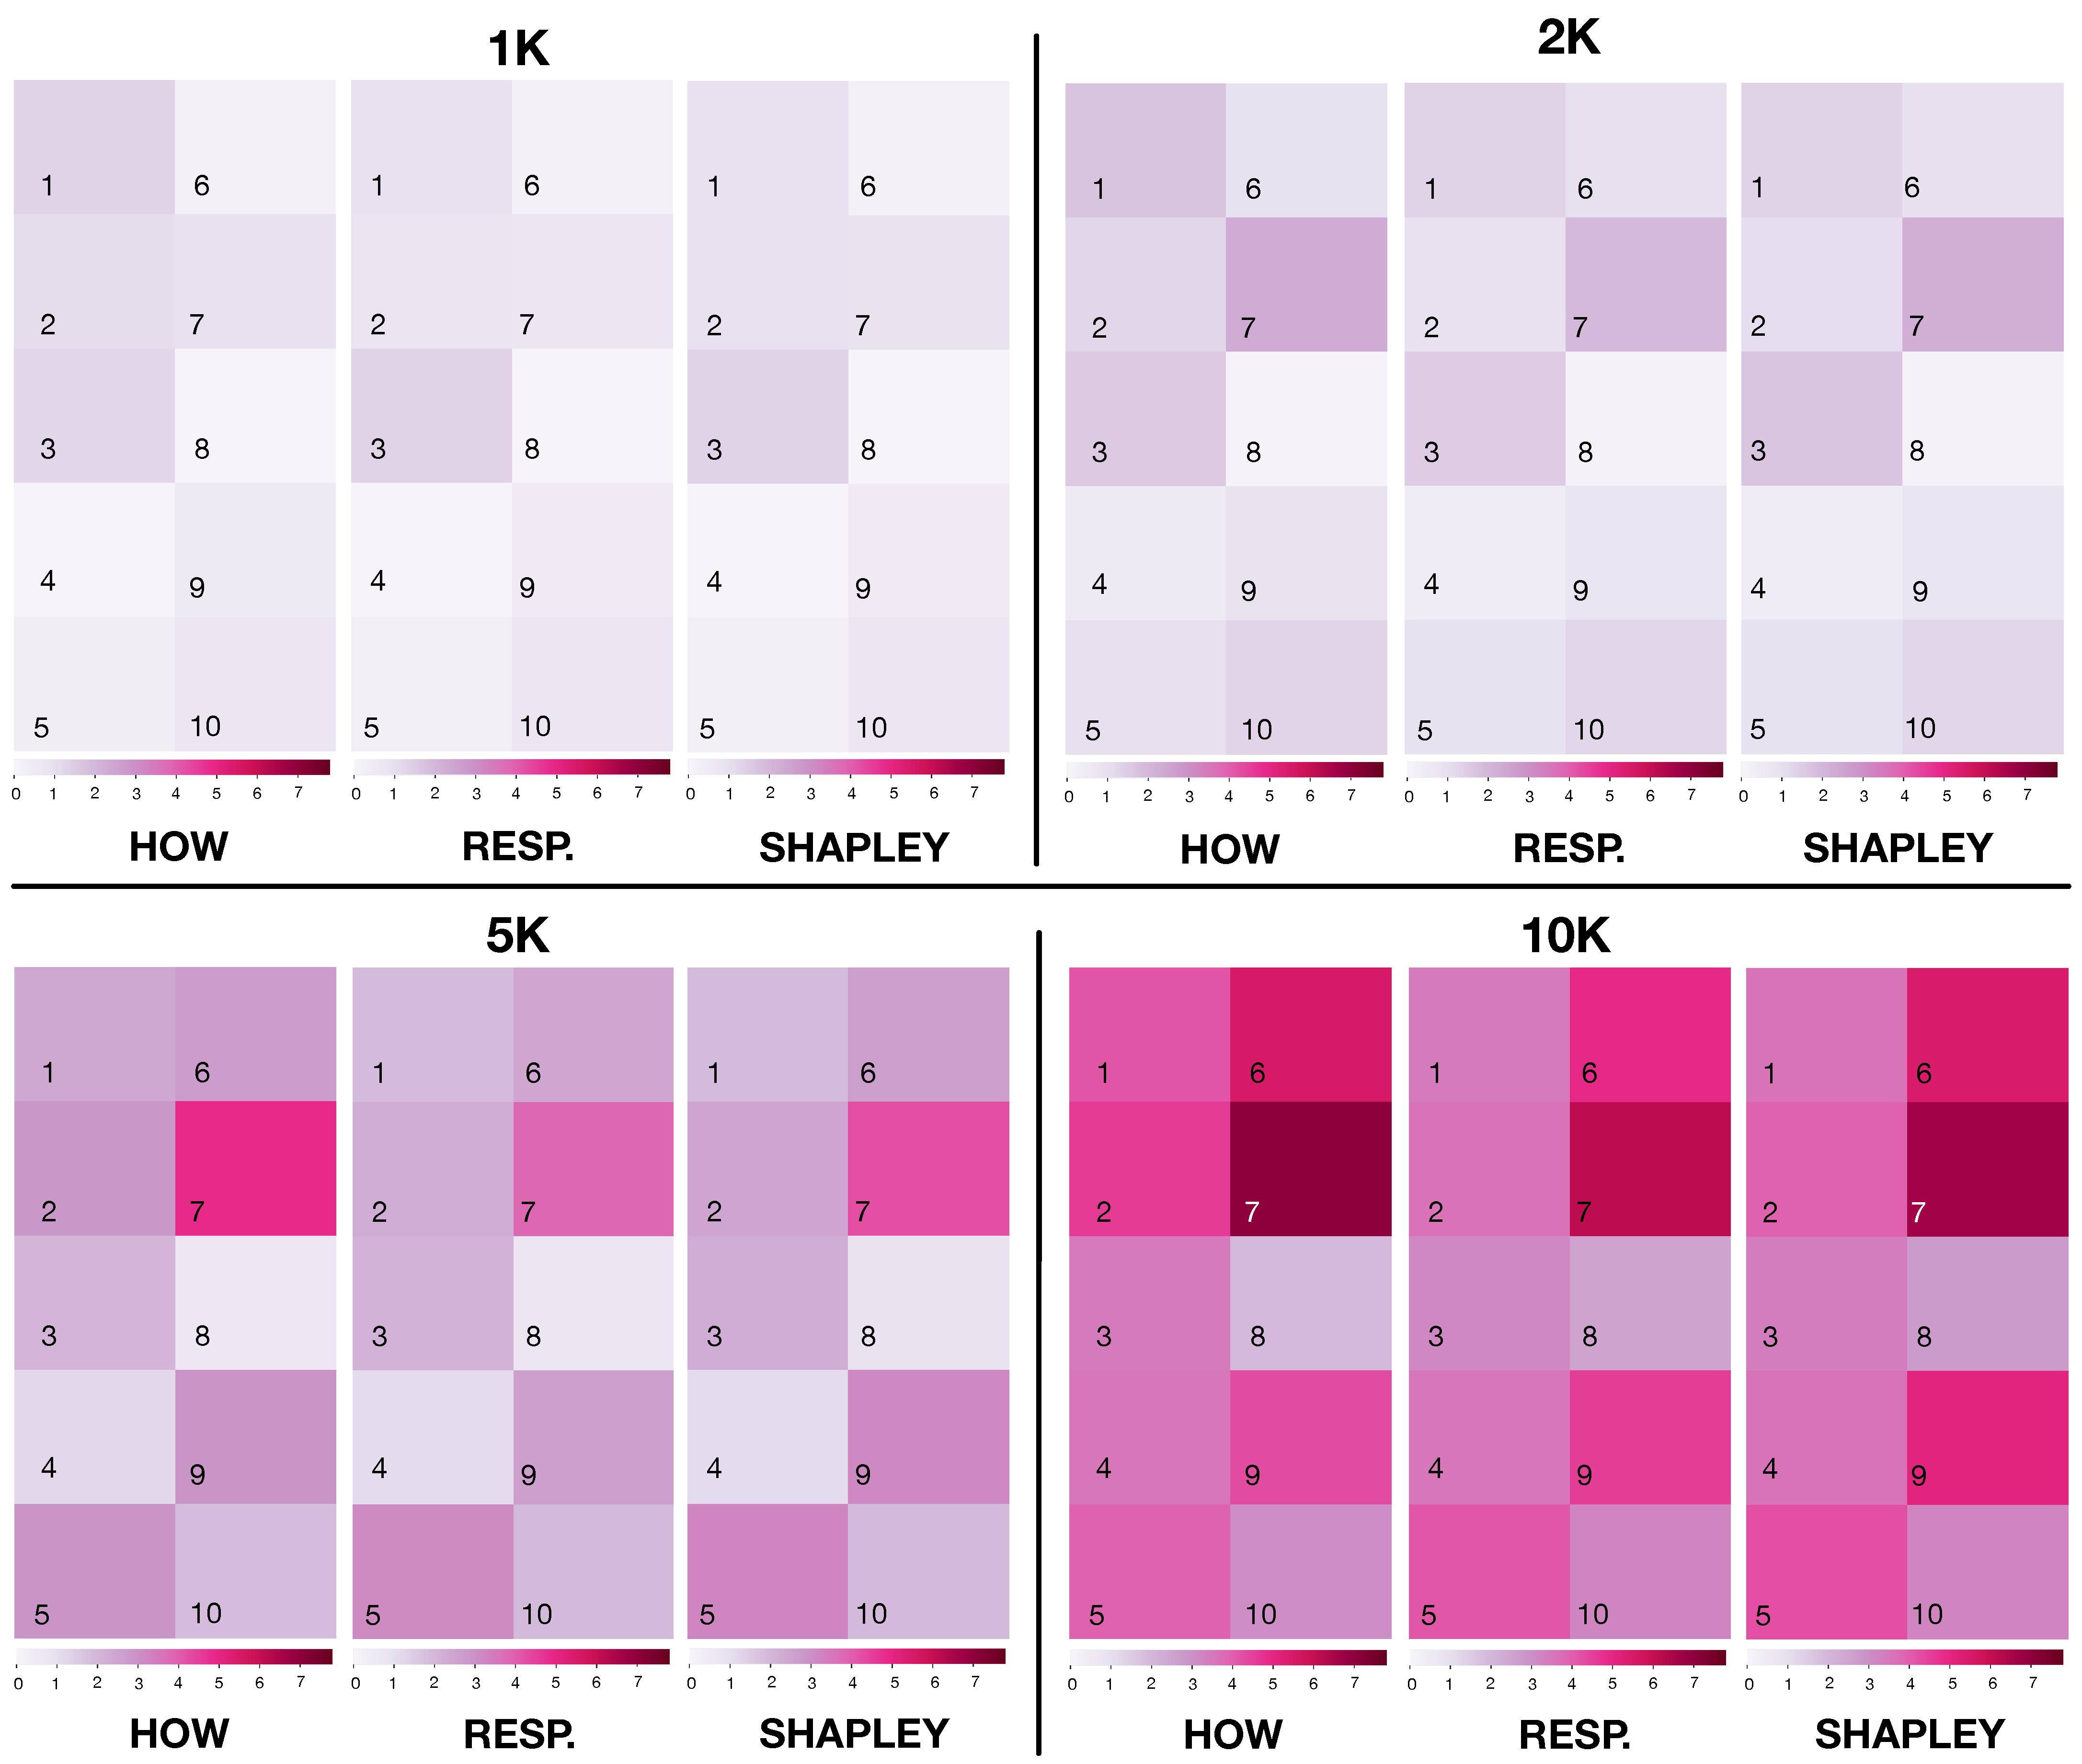
\includegraphics[width=.60\textwidth]{comparison}
  \caption{\rtwo{Comparison of the distribution of credit performed by the \rtwo{five} DSs on a subset of 10 tuples taken from the \texttt{family} table, simulating the passing of time. The number at the top of each group of heat-maps represents the number of polynomials whose credit has been distributed.}}
  \label{fig:comparison}
\end{figure}

In this figure, four groups of heat-maps are shown. Each group represents a ``snapshot'' taken %during an incremental accumulation of credit on the database 
after 1K, 2K, 5K and 10K provenance polynomials have been considered for credit distribution.  
The ten tuples in each heat-map  %from the \texttt{family} table, and
are those  highlighted in the \rone{yellow} boxes of Figure \ref{figure:comparison_on_synthetic_polynomials_2} from the \texttt{family} table.  


The polynomials used are the same as the experiment of the previous section. The range of credit in each map goes from 0 (no credit) to $7$ (the maximum quantity of credit reached -- using how-provenance -- on one of the tuples of the considered window at the ``snapshot'' with 10K queries). The color hue of the legend, as can be seen, still ranges from $0$ to $7.7$.

%\scream{I feel that this section is going into too much detail.  We should just get the big idea across.  I have "eaten" most of this text and tried to pull out the highlights. Don't bring up things unless you can explain them, or are trying to make a point.  The other problem is we can't really say why tuples wax and wane in overall credit -- it depends on the queries, which we don't go into (or want to go into).}

By the end of 1K queries, credit differentials between tuples as well as between strategies can be seen.  For example, tuple 3 is usually rewarded the most credit by all five strategies. 
\rtwo{Moreover, it can be seen that tuples $1$ receives a higher quantity of credit when how-provenance is adopted, showing how this form of provenance behaves differently from the others in this context}.
Moving to $2K$ queries, it is possible to see that tuple $3$ and $7$ are still the most rewarded by the strategies.

By the end of 5K queries, tuple $7$ emerges with the highest value of credit with all five DSs, a position which is strengthened with 10K queries. Moreover, with the passing of time, tuple $3$ ceases to be one of the most rewarded ones and new tuples, such as $6$ and $9$, emerge as being particularly rewarded at 5K, while at 10K tuples $6$ and $7$ are the most rewarded from the distributions.
This is because tuple $7$ is used several times within queries being executed, which is rewarded strongly by why- and how-provenance.
\rtwo{We also note that the responsibility-based distribution confirms its trend of being similar to why-provenance, although not identical. This is more evident at step 10K, where tuple 7 is slightly less rewarded using responsibility ($6.12$) with respect to why-provenance ($6.24$). 
The responsibility that rewards the more tuple $7$ is the one based on how-provenance (credit $7.03$), followed by the Shapley value (credit $6.64$).
This is due to the fact that tuple $7$ had, among some of the polynomials being used for the experiments, a high responsibility but it did not appear in all witnesses. This changed slightly the distribution.}


While the relative value of credit ``positions" of tuples within a DS strategy depends on what queries are being executed, the important thing to notice is the difference between the DSs over time:  overall, lineage gives less credit to tuples in the \texttt{family} table than the other strategies since credit is shared with tuples in other tables.
The other strategies recognize the more important role being played by the \texttt{family} tuples than those in the other tables.
\rtwo{The differences between why- and responsibility-based DS are, for the most times, negligible.} 
The differences between the why- and how-provenance-based DSs are also relatively minor in most cases. However, there are certain situations in which the role of a tuple is particularly critical in a query, and in this case the difference in the value of credit assigned is notably higher for how-provenance \rtwo{and the Shapley value}, as we saw with tuple 7 in the example of Figure \ref{fig:comparison}. 


\eat{
Focusing on the 1K and 2K groups, we see that credit distribution by the three DS are very similar, but that there are small differences.
We note that, in the 1K group, tuple 4 has the highest value of credit within all three strategies. Moving to the 2K group, tuple 4 still has the highest value of credit, although it has the highest value with the why-provenance DS; the other two strategies rewarded it less. 
In contrast, why-provenance and how-provenance rewarded tuples 2 and 3 more than the strategy based on lineage. 
Tuple 5 appears to be rewarded more by why-provenance and less by how-provenance, and even less by lineage. 
\scream{I don't understand what a "lower value of polynomial" is?  Do you mean lower number of queries?}
This shows that, even with these lower values of polynomials, that the strategies may differ and reward certain tuples more than others. 
We see the tendency of the lineage DS to reward tuples in this table less than the other strategies, since it does not take into consideration their importance. 
Instead, the DS based on why-provenance rewards more tuples like 4 and 5 (values 2 in both cases). 
The same can be said of the strategy based on how-provenance. However, in this case, tuples 4 and 5 are rewarded a little less (with credit values of 1.9 and 1.5 respectively). This is due to the fact that how-provenance contains more information. Thus, this DS rewarded more other tuples in the other used tables. Viceversa, tuples 2 and 3 are rewarded more by how-provenance DS (values 1.5 and 1.6) that the why-provenance DS (value 1.3 in both cases), due to the fact that their roles in the polynomials are more important.  
}

\eat{
Moving to the 5K group, we see how credit was accumulated on the tuples. Now tuple $2$ is the one with the biggest quantity of credit in this window. This shows how credit is able to track how the importance of tuples changes over time. 
In this group we see of it is more evident the difference between the distribution based on lineage and the other two strategies. The why-provenance and how-provenance based DSs appear to work similarly, that is to give similar values of credit to the same tuples. 
We can still see differences, for example on tuples like 8 and 6, that are more rewarded by the DS based on lineage.}

\eat{
Similar observations can be seen for the 10K group. We see how tuple 2 is still highly rewarded by all three provenances. In the case of lineage, however, it is at the same level with tuples 3, 4, and 8, while the other two strategies reward it the most. 
Once again we see the DSs based on why- and how-provenance operate similar distributions (we still note differences of few decimals between the values assigned to the tuples). However, it is still possible to see how tuples like $9$ are more rewarded by one DS, in this case the how-provenance one, than the other. 
This shows how the last two DS operate in a similar way. The differences between the credit assigned to the same tuple is of few decimals between the two strategies in most of the cases. However, there are certain situations when the role of a tuple is particularly critical in a query. This information is captured by the provenance polynomial, and this is why in certain cases the differences in the credit assigned to one tuple is notably different between the two strategies.  
}


To sum up, the DS based on lineage is sufficient to highlight which tuples in the database are used by a query, and distributes credit equally to these tuples. The resulting distribution rewards tuples that are used by more queries, but does not reward how many times tuples are used in the same query.  
However, a DS based on why-provenance, \rtwo{responsibility, Shapley value} or how-provenance may be better if the queries are complex, since they reward more tuples that have a critical role in generating the output. %These two DS are sensitive than the DS based on lineage (and the DS based on how-provenance is more sensible than the one based on why-provenance). 
\eat{Using the why-provenance and how-provenance DS, it is possible to change the distribution of credit to the tuple, rewarding more the tuples that have a more critical role in generating the output. The distribution based on how-provenance is most of the times similar to the one based on why-provenance. 
However, in certain instances, it differ from the other one due to the specific role of a tuple, an information that is present in the provenance polynomial but lost in the witness basis. }
In particular, these \rtwo{four} DSs may be useful for finding ``hotspots'' in the database based on the role of tuples, with the how-provenance-based and Shapley value-based DSs being preferable if a higher sensitivity to the role of a tuple in queries is required. 

%In particular, the DS based on why-provenance rewards more the tuples that are used in different ways by queries (i.e. are members of more witnesses). The DS based on how-provenance also takes into consideration how many times a tuple is used, adding even more sensibility to the distribution. 
%One may choose one other the other depending what are the aspects he wants to highlight in the data.

%%%%%%%%

\subsection{Credit vs Citations}

\begin{figure}[]
\centering
  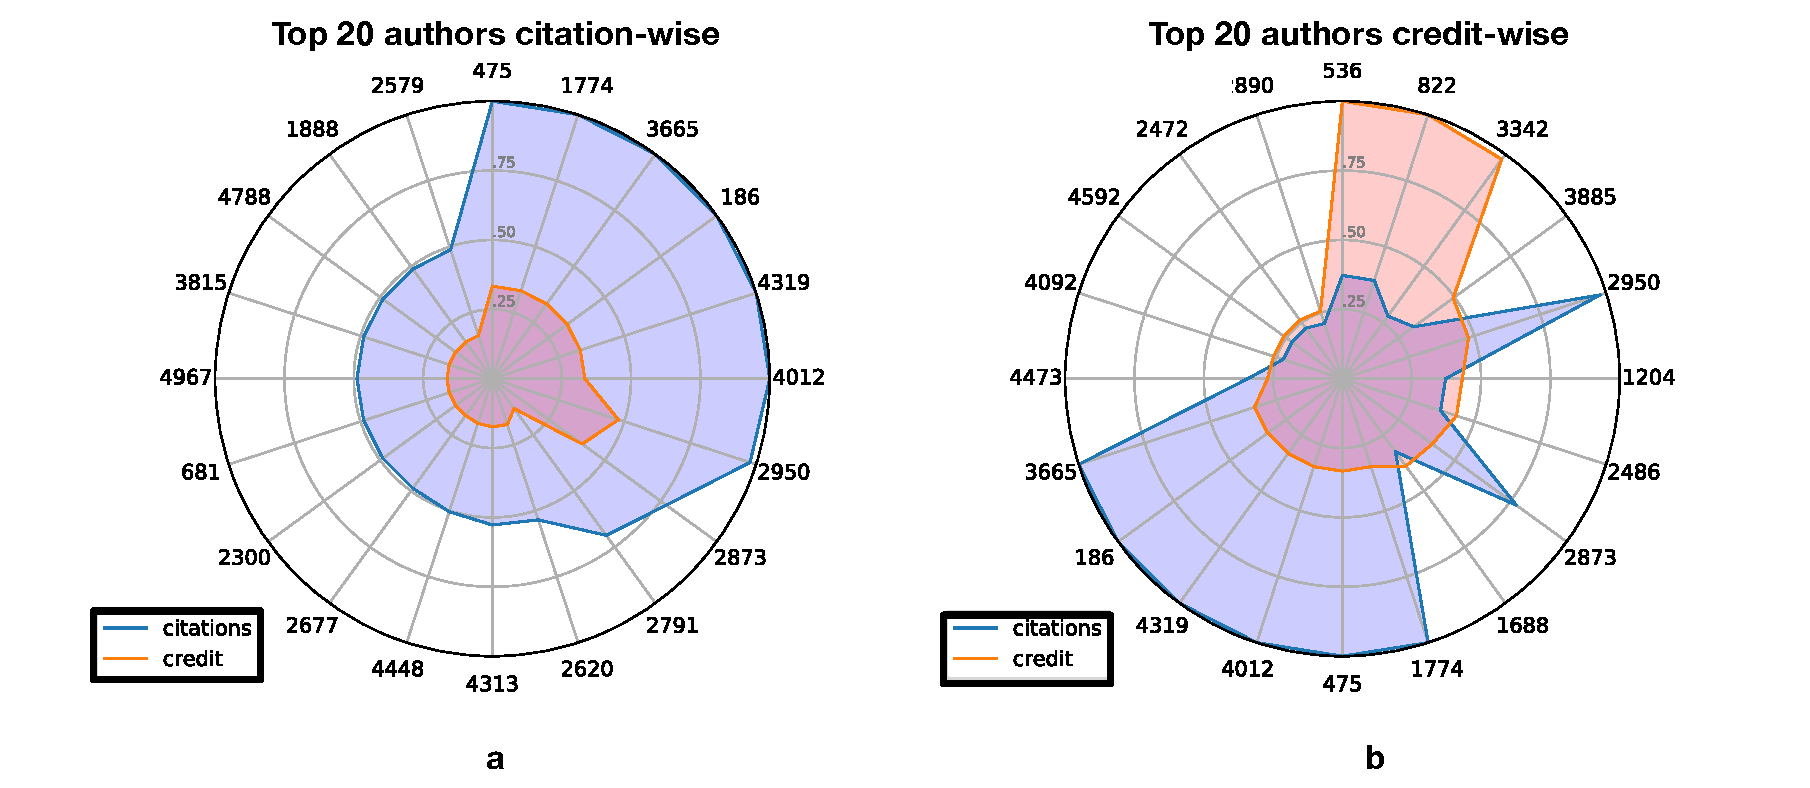
\includegraphics[width=1\textwidth]{2_radars}
  \caption{Radars presenting the top 20 authors citation-wise and credit wise, together with their (normalized between 0 and 1) values of citations and credit.}
  \label{figure:2_radars}
\end{figure}

In the last set of experiments, we compare traditional citations to the proposed credit distribution strategies to see the difference in reward for data authors and curators.  
\textcolor{correction}{Using both real-world and synthetic queries, we distribute credit to the authors responsible for the data under the different strategies. Our results show that credit rewards authors of data that is cited fewer times, but that has a higher impact on the query results.} 
%\scream{Reprise from the intro exactly what this is doing and why.}

\textcolor{correction}{To do so, we need to identify a set of authors and queries that cite data curated by them.}  
Considering GtoPdb, each target family page has a list of curators, representing the people who are co-creators and curators of the data comprising the page. This list can be obtained using the last query shown in Figure \ref{figure:family_structure}. 
Each time a target family page is cited, we assign one {\em citation} to each author associated with the page.  The authors also receive {\em credit} in the amount assigned to the data used by the query to construct the webpage, equally divided between the authors of the webpage.


\paragraph{Results: Real-world queries}
As described in Section \ref{sec:real_world_queries}, we consider real-world queries taken from papers published in the BJP which reference webpages in GtoPdb.
Since for these queries there is no difference in the distribution of credit between the DSs, only one value for credit is used.
%given in Figure \ref{figure:2_radars}. \eat{As we said, each time a webpage is cited, the authors of that webpage receive one citation, and also receive a quantity of credit that is equal to the credit assigned to the data and generated from the citation, equally divided among them.} 

The results are shown in the radar plots of Figure \ref{figure:2_radars}, in which each number on the outer circle (e.g. 475, 1774 and 3665) represents an author (id) and the blue (red) line represents the normalized value of credit generated by citations (credit), respectively. The first radar plot,
Figure \ref{figure:2_radars}.a, shows the top 20 authors in terms of {\em citations}, ordered in a clockwise direction, whereas Figure \ref{figure:2_radars}.b orders the authors based on {\em credit}. 
Comparing the author ids used in the outer circles of these two plots, it can immediately be seen that the ``top authors'' are very different using these two metrics, although there is some overlap (for example, authors 1774, 475, and 4012). 

%\scream{I don't understand what you are trying to say here.  Rewrote, putting old in eat in case I am wrong.}
Diving a bit deeper to focus on the red and blue areas in each of the plots reveals that there is a significance difference between citations and credit:
The top 20 authors in terms of citations do not have the highest values of credit (Figure \ref{figure:2_radars}.a).  Conversely, the authors with the highest values of credit do not necessarily have a large number of citations (Figure \ref{figure:2_radars}.b).
\eat{This is due to the fact that certain citations are more ``valuable'' in terms of credit, i.e. an author receive more credit from his/her citations, even if fewer, than other authors. This, in turns, happens because certain citations generate more credit than others. 
So, for example, author 536 presents the highest value of credit, although he is not even in the top 20 authors in terms of citations. This means that he receives much more credit from his relatively few citations than author 475. }
For example, author 536 has the highest value of credit, but is not even in the top 20 authors in terms of citations. This means that authors like 536, 822, and 3342 in Figure \ref{figure:2_radars}.b receive much more credit from their relatively few citations than authors like 475, who receives the largest number of citations.
That is, the data underlying certain webpages is more ``valuable'' in terms of credit than a citation to the webpage.  

\eat{Given how we prepared our experiments, the citations whose query produce more tuples, are also the ones that generate more credit, since we assumed that each output tuple carries credit $1$. Thus, the authors of the data returned by these queries are the ones that will receive more credit from these citations. Also, the authors that collaborated with fewer people will also receive a biggest share from the equal subdivision of credit. }

The reason for the difference between citation and credit is partly due to the experimental setup:  each output tuple carries a credit of $1$, and there can be many tuples used to generate a webpage.  Thus a webpage that is created from more tuples will have a higher credit value than one created from fewer tuples. Furthermore, authors who collaborated with fewer people will receive a biggest share of the equally divided credit.  However, all authors will receive a citation of one.

Credit distribution therefore rewards authors differently than traditional citations: an author who has curated larger quantities of cited data and collaborated with fewer co-authors, will receive larger quantities of credit. Thus, credit rewards them for their larger contribution to the database. 

%In other settings, where the quantity of credit can be computed considering different criteria, such as the impact of the cited data in the citing paper, credit distribution can help to identify with even deeper precision the data and the authors that contributed more to the scientific impact in the context defined by the considered citations.

%\scream{I "ate" the final paragraph. I didn't understand what other strategies you are talking about and thought it was more more in keeping with "future work"?}

%\begin{figure}[t]
%\centering
%  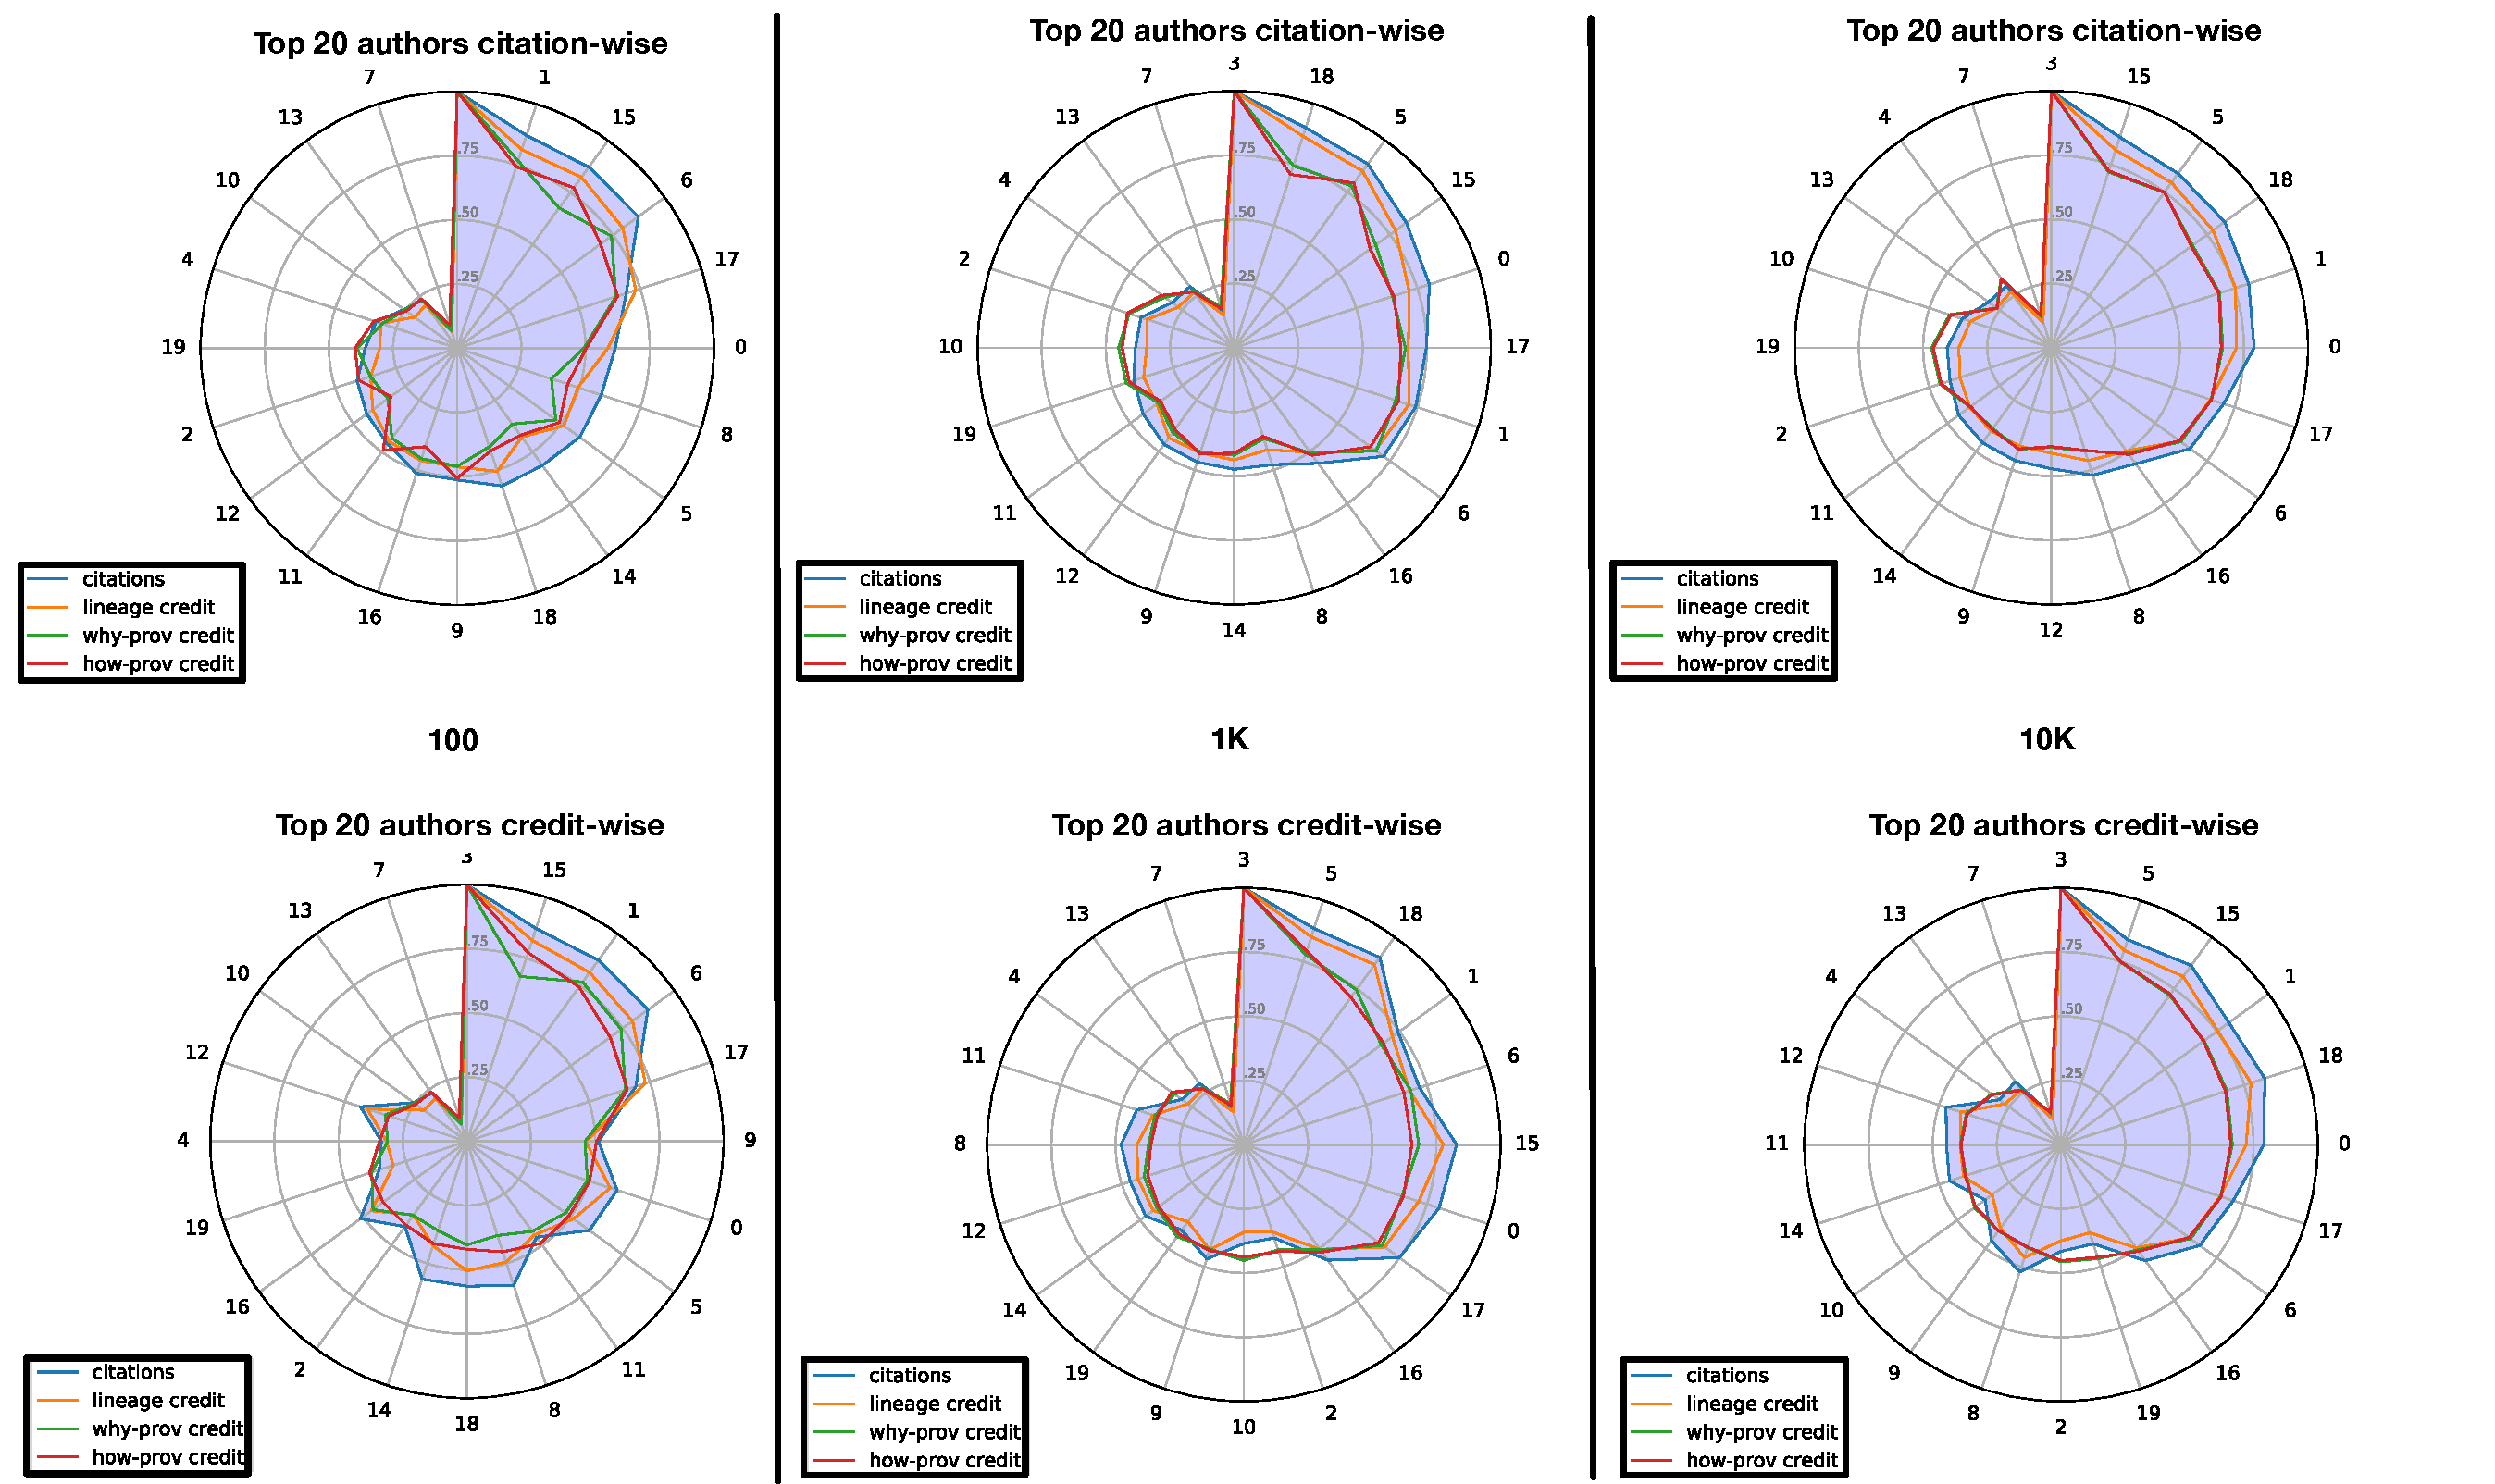
\includegraphics[width=1\textwidth]{figures/3_radars}
%  \caption{Radars presenting 20 authors ordered citation-wise and credit-wise, together with their (normalized between 0 and 1) values of citations and credit, through the execution of different numbers of polynomials (100, 1K, and 10K). The radar plots ordered by credit consider the credit assigned by the DS based on how-provenance.}
%  \label{figure:3_radars}
%\end{figure}

\begin{figure}[t]
\centering
  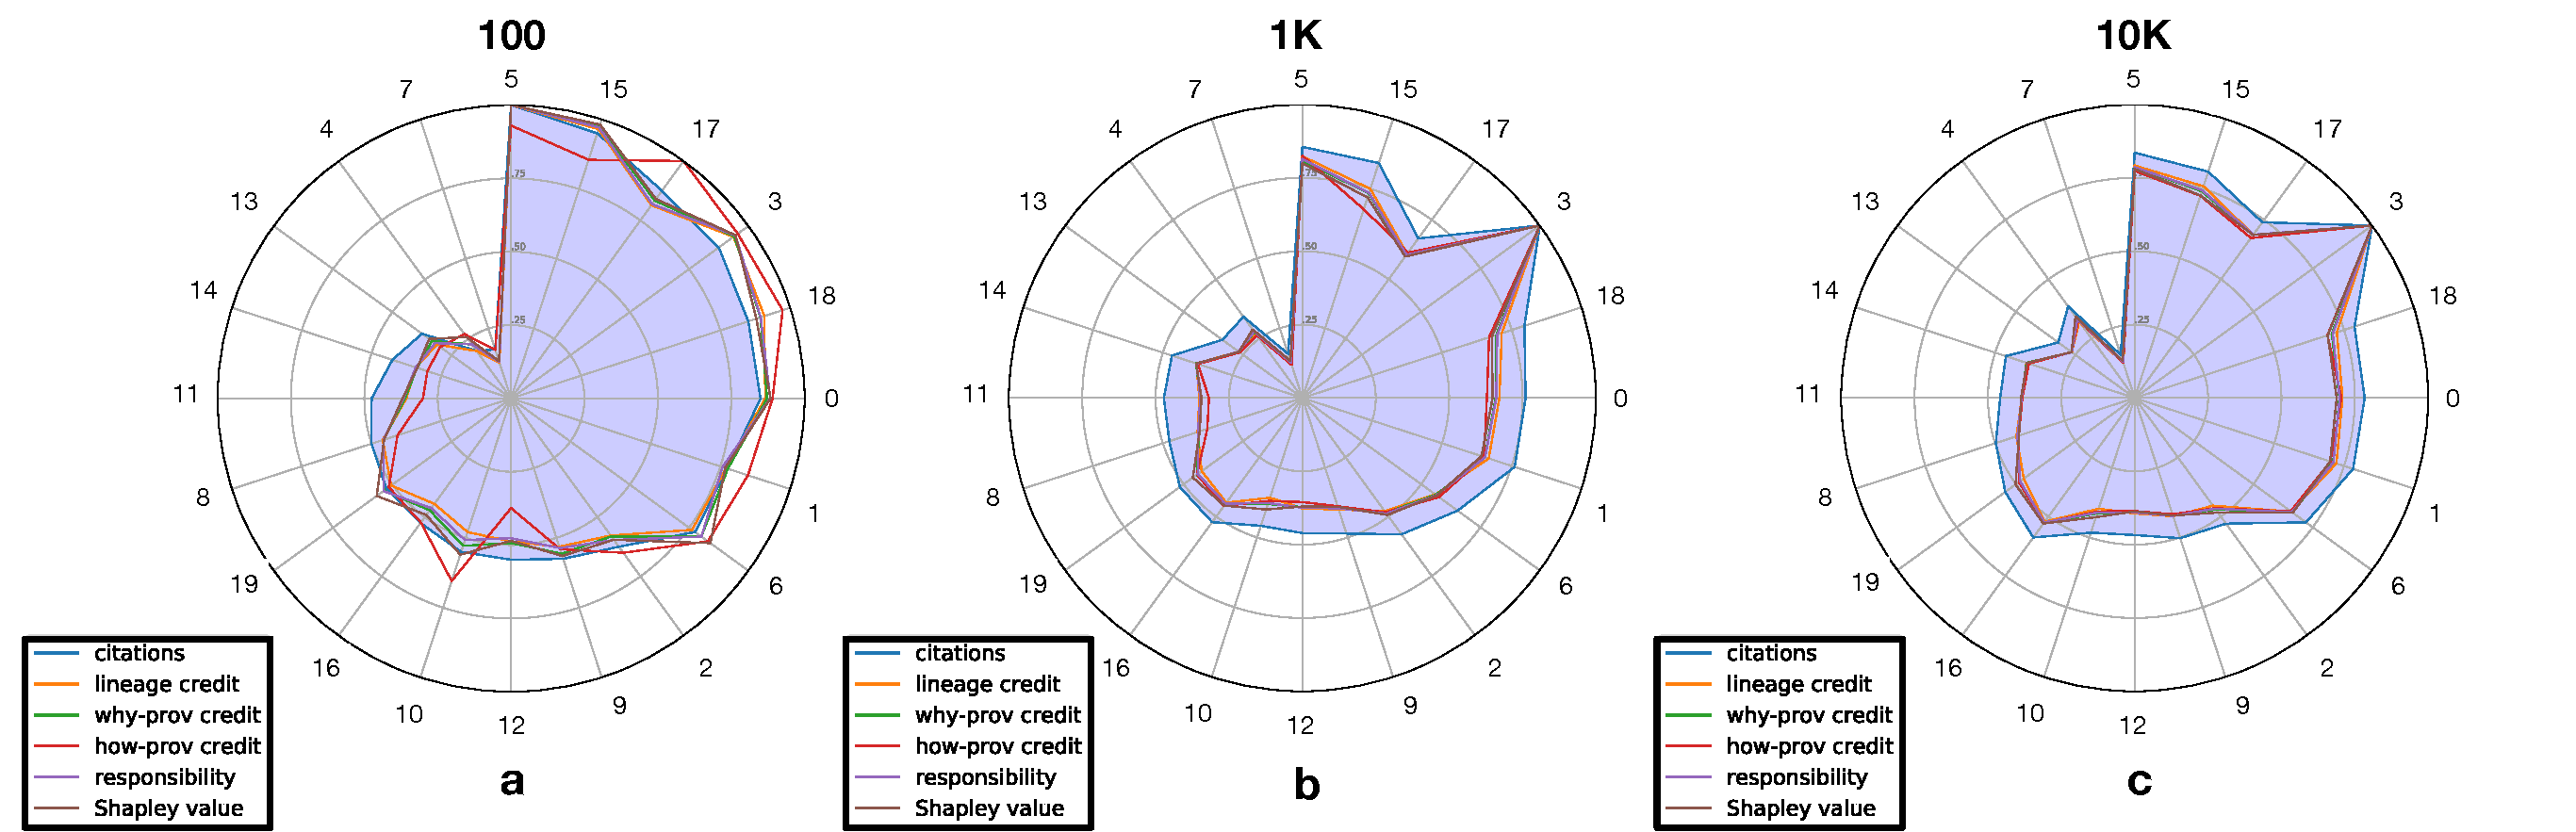
\includegraphics[width=1\textwidth]{radar}
  \caption{
\rtwo{  Radars presenting the 20 synthetic authors with corresponding citation and quantities of credit distributed through the 4 DSs (all values normalized between 0 and 1) through different numbers of polynomials (respectively, 100, 1K and 10K). 
  The order is the one defined by figure a, i.e. descending order of citations  obtained from 100 polynomials.}}
  \label{figure:3_radars}
\end{figure}

\paragraph{Results: Synthetic queries}
We used the same synthetic polynomials described in Section \ref{sec:synth_queries}, and we distributed credit with the first $100$, $1K$, and $10K$ of them.
Since these polynomials are created by randomly selecting tuples from three tables, they usually correspond to a set of data curated by  authors who, in reality, did not collaborate. To make the size of the author set more realistic, we therefore created $20$ synthetic authors, and randomly assigned one author to blocks of consecutive tuples in the database, with the size of each block varying between $10$ and $40$, to simulate different quantities of work performed by an author. 
Every time an author appears as curator of one or more tuples used in a polynomial, we assign them one citation.  
They also receive four kinds of credit, each one using a different DS.

Figure \ref{figure:3_radars} shows three radar plots, one for the results obtained with 100 polynomials, one with 1K polynomials, one with 10K polynomials.  
Each plot shows the top 20 authors in terms of citations (hence the authors and clockwise ordering is the same in each of the plots), and additionally shows the the normalized values of citation (blue line), lineage-based credit (yellow line), why-provenance-based credit (green line), how-provenance-based  credit (red line), \rtwo{responsibility-based credit (violet line), and the Shapley value-based credit (brown line)}. 

As can be seen, given the synthetic nature of the queries, the correlation between the number of citations and the quantity of credit assigned to the authors appears to be a much stronger than with the real-world queries of Figure~\ref{figure:2_radars}. In fact, for Figure \ref{figure:3_radars}.a  the linear correlation between the citation number and all four types of credit is always above 0.94 with p values in the order of 3e-8.
\eat{Nonetheless, it can still be seen that credit does not always follow the citation count. }
The credit distributed via lineage is closest to  the number of citations (a linear correlation of 0.99, p value of 2e-16 in Figure \ref{figure:3_radars}.a), while the other three types of credit behave slightly differently (a linear correlation of around 0.95 or above in all other four cases in Figure \ref{figure:3_radars}.a).  
Similar observations can be made for Figure \ref{figure:3_radars}.b and \ref{figure:3_radars}.c.

What these figures show is that, in certain cases, authors who do not have a large number of citations receive more credit than others, as for example authors 17, 18 and 10 in Figure \ref{figure:3_radars}.a, 
%or author 19 in Figures \ref{figure:3_radars}.b and \ref{figure:3_radars}.c, 
and especially when credit is distributed using how-provenance.
This again shows how credit gives a different perspective on the role of data and authors by going beyond the limitations of traditional citations.  

It is worth noting that, when scaling up to $1K$ and $10K$ polynomials, the credit distributions  become almost identical  
\eat{We note that, although not exactly overlapping, the values of credit assigned to the authors by those DS become quite similar with these higher quantities of polynomials, suggesting a sort of equivalence between the two DSs in this case, at least in the task of rewarding authors} (the linear correlation for the values of Figure \ref{figure:3_radars}.c is more than 0.99 with a p-value of 1.32e-32). This is consistent with what we observed in Figure \ref{figure:comparison_on_synthetic_polynomials_2}.


\eat{
\subsection{Execution time}
The last experiment compared the time required to calculate the credit distribution for the three strategies. The results are shown in Table \ref{table:times}.  

\begin{table}[hbt]
\centering
  \begin{tabular}{| l |c | c | c | c ||}
  \hline
    \# of polynomials  & lineage & why-prov. & how-prov. \\
    \hline
    100 & 226.6 ms & 192.0 ms & 185.5 ms \\
    200 & 431.2 ms & 392.2 ms & 403.2 ms \\
    500 & 1.013 s  & 934.2 ms & 881.8 ms \\ 
    1K  & 2.041 s  & 1.934 s  & 1.744 s  \\
    2K  & 3.773 s  & 3.491 s  & 3.510 s  \\
    5K  & 8.992 s  & 8.653 s  & 8.889 s  \\
    10K & 17.10 s  & 16.84 s  & 16.84 s  \\
    20K & 34.59 s  & 35.30 s  & 39.70 s \\
    100K & 3.289 min & 3.442 min & 3.652 min \\
    1M  & 35.91 min & 34.87 min & 37.91 min \\
    \hline
  \end{tabular}
  \caption{The times required to perform the three DS for different number of synthetic polynomials.}
  \label{table:times}
\end{table}

\scream{Perhaps you should plot these using lines?  It is not easy to see that it grows linearly.  Also, why is linage almost always slower than the why- and how-provenance?  How was the experiment performed?}
As can be seen, the execution time grows linearly with the number of polynomials that are submitted to the system. When there are a large number of polynomials (1M), the time required by the DS based on lineage and why-provenance is slightly less than the time needed for the DS based on how-provenance. This is due to the increased complexity of the how-provenance calculation.  \scream{How significant is the difference?}
We note that, since we created these polynomials on-the-fly, these values do not include the time required to compute the provenances.
Therefore, just taking into account the time required to distribute credit, the three DS are roughly the same in terms of performance. 
\scream{This seems a bit of a contraction to the previous claim of "increased complexity".}
Only when there are a large number of complex polynomials do lineage and why-provenance  become preferable to how-provenance in terms of execution time, but coming at the cost of a less equitable credit distribution strategy.
}


%\subsection{Discussion}
%
%In the previous sections we showed, through the use of different experiments, the behavior of credit and its distribution with the use of different DS. 
%It appeared that, in the case of SPJ queries, the three distributions behave in the same way on GtoPdb. 
%
%Using synthetic polynomials, we showed how the three DS actually behave differently, in particular with the passage of time, i.e. when more and more polynomials are processed. 
%The three DS are all effective ways to distribute credit, and there is not one distribution that is preferable to the other all the time. It all depends on the needs of the users. 
%
%Lineage is to be preferred when users only want to find tuples that are used in a database by queries applied to this database. With the accumulation of credit coming from many queries, the DS based on lineage is also able to create ``hotspots'' among the tuples of the relational database.
%However, lineage rewards equally the tuples used by a query.
% 
%Why-provenance is more versatile when users also want to consider how many ways a tuple is used; thus, in a way, its \emph{versatility} inside the queries that used it.
%Finally, how-provenance also counts how many times a tuple is used, its \emph{frequency} in the computation of a query. 



\section{Discussion}
\label{sec:discussion}
Before concluding, we discuss some design decisions:  the focus on Credit Distribution (as opposed to Credit Generation), and the choice of Distribution Strategies.

\subsection{Credit Generation}
\label{subsec: generation}
\rtwo{In this paper we focused on Credit Distribution, the problem of distributing credit generated by a citation to the parts of the database referenced by the query.
A different problem is Credit Generation, the task of generating credit which is then distributed. 
Credit Generation presents a series of issues which are shared by traditional citation practices. For instance, defining the  quantity of credit to be generated for a given citation is still an open problem. Different types of citations may generate different quantities of credit. 
Data cited as previous work or as useful for previous work may generate less credit than other data extensively used to produce the results presented in a paper. The computation of credit could be done manually (although we must consider the complexity of the task, human biases and the resources required to carry it out) or automatically, but it must be based on a shared definition of impact which is still not agreed upon for data or for traditional citation. For this reason, we used a uniform credit assignment.
}

\rtwo{There is also the problem of \emph{transitive credit distribution}, i.e., how to transitively propagate credit from one cited unit to another unit that was used to produce the one being cited. For this, 
%it is possible to envision 
a graph of cited units that propagate credit between the units depending on  influence could be used. How to propagate credit is an open and non-trivial problem that needs to consider the importance and impact of a citation in a work, be it a paper or data, and how to eventually compute the quantity of credit to be propagated.}


%\todo[size=\scriptsize]{GMS: I commented out a list of items I did not agree much with. Please take a look and resume what you think is good for you (if any). -- DD: Some of the points were raised because of Reviewer 2. Since we discuss about them in the first paragraph, we can keep the list out of the paper. I added another paragraph to add more meat for reviewer 2, it can be removed too.} 

%% list commented OUT (11 Dec 2021)
\eat{
\begin{enumerate}
	\item \emph{How much credit should be generated?} Different types of citations may generate different quantities of credit. Data cited as related to the results or as useful for previous work of a study may generate less credit than other data extensively used to produce the results presented in a paper. The computation of the credit could be done manually (even though we must consider the complexity of the task, human biases and the resources required to carry it out) or automatically, but it must be based on a shared definition of impact which is still far from reaching both for data and traditional citations. For this reason, for the time being, a uniform credit assignment looked more appealing and realistic to us.\todo[size=\scriptsize]{GMS: commented out the part about NLP; it does not make sense to me. and removed self-citations, that's debatable, not data specific and we do not want to go there.}
	%Different techniques may be employed to compute credit reflecting the impact of the data being cited. The manual annotation by the authors of the data that are more relevant to the economy of the paper is a possibility . Some forms of automatic annotation could be or computations performed through NLP techniques to infer the importance of a citation based on the context of the text where it is cited.
	%\item \emph{Credit produced by self-citations} Data credit, being built on top of traditional citations, inherits some of its problems. Authors, using self-citations, may generate and distribute credit to themselves, making their work appear much more impactful that it actually is. Different strategies may be exploited in this scenario, ranging from ignoring completely the credit generated from self-citations to applying a discount factor to control it.
	\item \emph{Generic citations} As we mentioned, citations may go to the whole database, or to views of the database computed using a big portion of its data. In this case, credit may be assigned indiscriminately to large portions of data, losing the ability to accurately identify parts of the database that have high impact. In this case it is also possible to ignore queries that are too ``general'' and considering only queries that are discriminative enough.\todo[size=\scriptsize, color=green]{this is not about credit generation but distribution. I do not think this is needed (+ I do not know if I agree with this. remove?)}
	\item \emph{Different types of credit} In the real world, there are different types of research communities interested in information in a database. Doctors' interests and queries may differ from the interests and queries of ophthalmologists or pharmacists. For this reason, only distributing one generic credit generated from all possible queries coming from this heterogeneous set of users may simply highlight data that are important in general, without taking into consideration the specific their specific and different needs. One possibility is to keep separated the credit generated by different types of users, e.g., have one type of credit generated from queries coming from doctors, another type of credit generated from queries submitted by ophthalmologists, etc. In this way, it will be possible to accurately tailor the process of credit distribution around the information need of different categories of users. 
\end{enumerate}
}


\eat{
\rone{Finally, in our experiments we assumed that the credit carried by an output tuple is one. Thus, each tuple in the output has equal importance. As described above, this assumption may be revised and different credit to different output tuples could be assigned.}

%% again? redundant with above
%This in general may not be true, since different tuples in the output may have different weight, depending on the context of the citation. For example, data that is fundamental for the results of a paper may have more credit than data being cited as a reference. 
%\emph{Credit generation}, i.e. the process by which the credit of the output tuples is decided, is a research problem with its own dignity and complexities, and we did not face it in this paper.}

\rone{Nonetheless, from the distribution models viewpoint no change is required since the DCD is defined for a generic value $k$. Of course, note that if the quantity of credit carried by an output tuple changes, as a consequence the final distribution will change too, since certain tuples will be more ``impactful'' (i.e., distribute more credit) than others.}
}

\rone{Finally, in our experiments we assumed that the credit carried by an output tuple is one. Thus, each tuple in the output has equal importance. As described above, this assumption may be revised and different credit to different output tuples could be assigned.  Note that from the distribution model viewpoint no change is required since the DCD is defined for a generic value $k$. }



\subsection{Choice of Distribution Strategies}
\label{subsec: DSs}
\rone{In this paper we presented four different DSs, so the natural question is which one to use.  This depends on the task at hand.   When we want to highlight the tuples being used in the database by a workload, the lineage-based DS may be sufficient. When we also want to know the relative impact of tuples in the context of the query, the other DSs should be used since they give a better understanding of the importance of data.}

% \todo[size=\scriptsize]{GMS: Not superconvinced of the following paragraph. is it good to talk about SPARQL when we say that relational DBs are still widely used? Alternative example with SQL? Or do we just remove it?}
\rone{In the real-world based experiments, the four DSs behaved the same, which was due to the specific nature of the data and the queries being used. However, the why-provenance of a query will differ from the lineage of the same query whenever the output tuples can be computed in more than one way by the query, i.e., if there is more than one witness. This is usually true when join and projection operators are used in the query.
% There are several situations where the user-submitted queries present different distribution of credit.
% For instance, the work by \citet{BonifatiMT17} showed that in the context of SPARQL query logs submitted to various databases such as DBpedia and Wikidata, more than $90\%$ of these queries are of type select, and of those more than $30\%$ perform join operations through the \texttt{and} operator. These queries contain triple patterns with cardinalities that range from one to eleven triples, thus showing some complexity that can be caught by why- and how-provenance based DSs.
} 

%\scream{SBD: this paragraph went all over the place and was confusing.  I eliminated a lot of details that you might think are important (original is in an eat environment.}

\rone{To address the question of what types of queries are likely to extract cited data, we turn to the results of published studies on the characteristics of query workloads and the complexity of their queries~\cite{Vogelsgesang2018get,Remil2021makes,Jain2016sqlshare}.  
These studies show that operations such as inner-/outer-joins and projections occur in a significant number of queries.  Therefore why- and how-provenances may become quite complex in certain cases and provide a distribution of credit that is significantly different from the one obtained with lineage. }


\eat{
\rone{To address the question of what types of queries are likely to extract cited data, we turn to the results of published studies.  In \cite{Vogelsgesang2018get}, which studies the characteristics of query workloads and the complexity of their queries, they showed that operations such as inner joins can be found in at least $4.5\%$ of queries in the considered workload, %with a maximum number of times the operator is used in the same query equal 
and used up to to $164$ times in the same query. Outer joins were found in $1\%$ of the queries, and used up to $247$ times in the same query. }
\rone{\cite{Remil2021makes} showed that in the query workload of one company 520 queries out of 140K used joins, while 3470 used projections. }
\rone{\cite{Jain2016sqlshare} shows instead that 11\% of the queries in their  workflow used outer join. Moreover, 2.5\% of the considered views access other datasets, and 10\% of the queries logged in the system access datasets that the query author does not own. It also showed that many queries are short in their considered workload in terms of ASCII characters being used (circa 20\% are under 100 characters), on the other hand the longest query range up to 11375 characters. The simple length is not necessarily equivalent to complexity, thus the authors also showed that, while many of the considered queries have less than 4 distinct operators, a percentage around 30 and 60\% of queries, depending on the workload, present a number of distinct operators between 4 and 8. Finally, the considered queries also showed a higher entropy, i.e., they were particularly different among them.}

\rone{
These works provide us evidence of the fact that, potentially, why- and how-provenances may become quite complex in certain cases and provide a distribution of credit different from the one obtained with lineage. 
}
}

% \scream{Is there more to say here? What are the general queries for which responsibility is hard to compute, and can the various provenances handle them at all?  I know that provenance semi-rings has been extended to SPJU and aggregate queries, so imagine this means the others can be extended since it is a general framework. -- DD: added more information from literature and comments}    
\rtwo{From a computational complexity standpoint, all five DSs are similar since we focused on SPJ queries. Going beyond SPJ queries, \citet{howProvenanceGreen} proposed the provenance semiring framework for SPJRU (Select, Project, Join, Rename, and Union queries), and \citet{AmsterdamerDT11} showed how to extend the framework to aggregate queries.
\eat{ queries, thus we could expand our approach to those types of queries too.  \citet{AmsterdamerDT11} showed that it is also possible to compute provenance polynomials for aggregate queries by annotating with provenance tokens also the \emph{individual values} within the tuples, using provenance to describe the values computation. 
} 
Since lineage and why-provenance can be computed starting from how-provenance, it is possible to apply the first three DSs proposed in this paper to SPJRU and aggregation queries.} 
\rtwo{Causality and subsequently Responsibility are harder to compute (NP-complete~\cite{MeliouGMS11}) for general queries. Credit Distribution is more concerned with Responsibility, which is in general hard to compute~\cite{ChocklerH04}. \citet{MeliouGMS11} proved a dichotomy result for conjunctive queries: for each query without self-joins, either its responsibility can be computed in PTIME in the size of the database, or checking if it has a responsibility below a given value is NP-hard. Queries with self-joins are NP-hard in general. This makes responsibility harder to be utilized for credit distribution in a real-world application, since for this problem it is necessary to actually know the responsibility value, not simply the ranking amongst tuples.}

\rtwo{As for the Shapley Value, \citet{LivshitsBKS20} studied the computational complexity of calculating the Shapley values in query answering. They originally showed mainly lower bounds on the complexity of the problem, with the exception of the sub-class of self-join free SPJ queries called \emph{hierarchical} queries, where they gave a polynomial-time algorithm. 
Very recently, \citet{DFKM22} proved that the Shapley value can be efficiently (polynomial-time) reduced to probabilistic query answering. This not only applies to hierarchical queries, but to general SPJ queries. This means that one can compute Shapley values using a query engine for probabilistic databases, for example, the practically effective \emph{Knowledge Compilation}~\cite{JhaS13}, making it a viable solution for Credit Distribution via SPJ queries.} 

\eat{
Another promising DS that could be developed is one based on Shapley values. This function has been widely used in knowledge representation and machine learning, and has strong theoretical justifications.  However, its use in databases as a metric for quantifying the influence of a tuple on the output of a query (thereby presenting an alternative to responsibility) has only recently been proposed~\cite{LivshitsBKS20}.    Furthermore, the initial theoretical analysis in~\cite{LivshitsBKS20} showed mainly lower bounds on the complexity of the problem, and did not suggest a feasible implementation.  However, very recently, an efficient implementation for Boolean queries (queries that output true or false) has been provided~\cite{DFKM22}, both in terms of an exact computation (which in practice works well for most queries) and an inexact one (which is extremely fast and provides the same ranking of tuples as the exact computation, but not necessarily the same values).  In future work, we will explore a Shapley-based DS and test its performance in Credit Distribution.}


\eat{
In particular, Shapley has (at least) four properties that are widely believed to be important:
\begin{enumerate}
\item 
Efficiency:  The sum of the Shapley values of all agents equals the value of the grand coalition, so that all the gain is distributed among the agents.  
\item
Symmetry:  If i and j are two actors who are equivalent in the sense that v(S U {i})= v(S U {j}) for every subset S of N that contained neither i nor j, then their Shapley values are the same.
\item
Linearity:  If two coalition games described by gain functions v and w are combined, then the distributed gains should correspond to the gains derived from v and the gains derived from w.
Shap_i(v+w)= Shap_i(v) + Shap_i(w) for every I in N.  
Also, for any real number a,  Shap_i(a*v)=a*Shap(v)
\item
Null player:  The Shapley value of a null player i in a game v is zero.  A player i is null if v(S U {I}) = v(S) for all coalitions S that do not contain i. 
\end{enumerate}

The provenance-based approaches certainly satisfy 1and 4, and I believe that at least why- and how-provenance satisfy 2.  However, they don’t satisfy linearity (Nave gave me a counterexample for this).
}




\section{Conclusions and Future Work}
\label{section:conclusions}

This paper 
%expanded on our previous work on data credit and data credit distribution in \cite{dosso2020data} by 
defines four new distribution strategies based on why-provenance, how-provenance, responsibility, and the Shapley Value, and it compares them against the lineage-based distribution strategy defined in \cite{dosso2020data}. 
The first, why-provenance-based DS, uses the concept of a witness, and gives more credit to tuples that appear in more than one witness. 
In this way, tuples that are more important to the query and are used in different ways are rewarded more. % by the strategy.
The second, how-provenance-based DS, considers the frequency with which a tuple or combination of tuples is used in the query through the information contained in a provenance polynomial. In this case, the how-provenance-based DS is more sensitive than the why-provenance-based DS to the role and importance of tuples.
\rtwo{The third DS exploits the notion of responsibility, a real value that ranks the lineage tuples based on their degree of causality in generating the output. The responsibility-based DS was shown to behave similarly to the why-provenance based DS.}
\rtwo{The fourth DS uses the Shapley value function, used to rank the facts of the database, seen as players, in producing the required result. To do so, the wealth function in the Shapley value's definition was adapted for general free-variable queries on the database.}

To show the differences between the five DSs, we performed extensive experiments based on GtoPdb, a curated scientific relational database, using both real and synthetic queries. 
In the first set of experiments, we used select-project-join (SPJ) queries extracted from citations to webpages in GtoPdb found in papers published in the British Journal of Pharmacology. 
Using these ``real" queries, we distributed credit to tuples in different tables of the database, highlighting tuples that were more frequently used. 
We showed that, with these queries, the five strategies produce the same distribution. This is because the SPJ queries were fairly simple, and did not use self-joins. Therefore the formulas underlying the different DSs had the same output.

In the second set of experiments, we synthetically produced more complex provenance polynomials, corresponding to more complex queries, that resulted in exponents and coefficients in the provenance polynomials that were greater than (or equal to) $1$.
These experiments highlighted the differences between the five DSs.
\eat{
In this way, we showed that, even though all three DS can highlight all the tuples used by the queries in the database, the three have different behaviors. }
\rtwo{While the DS based on lineage rewards all the tuples used by a query equally, the strategies based on why-provenance and responsibility give more credit to  tuples that are more critical to the query.
In particular, why-provenance considers the different ways in which a tuple is used in a query, while responsibility considers the relative importance of a tuple in the generation of the output.}  
\rtwo{The DS based on the Shapley value similarly rewards the tuples based on their participation. The more impactful the role of a tuple, the higher its reward in credit. This distribution proved to be different from the previous two and to reward even more tuples that are used in more than one witness.}
How-provenance is even more sensitive to the tuple's role: it also considers the frequency with which a tuple or a set of tuples is used. %in the case of more complex queries. Depending on the goal of a user, one provenance may be preferred to another. 

In the third set of experiments, we showed how the differences between the DS are compounded over time, i.e. when more and more queries are processed by the system.

In the fourth set of experiments we compared traditional citations to authors to the credit accrued to them via the DSs. We showed how, in both real-world and synthetic scenarios, credit rewards authors 
who contribute/curate data that has the highest impact, and therefore receives the biggest quantity of credit, and not necessarily the data with the highest citation count. 
%\scream{I don't really understand this point.}
In this sense, credit appears to be an useful new measure to discover data and their corresponding curators that have a high impact in the research world, even when they are cited few times or do not appear at all in the data that are cited (i.e. the case of data used to build the output of a query but that is not visualized in the output itself).

 
\eat{
In more complex and sophisticated scenarios, where different strategies may be implemented to decide the generated quantity of credit to be distributed, new factors beyond the only ``quantity'' of curated data can be factored in in rewarding data curators.
The result will be a distribution of credit that represents even better the actual work and worth of data curators and their impact in the scientific community.}
\eat{
\screams{I reworded to this.}
Other, more sophisticated, strategies could also be used to decide how credit is distributed between the authors, beyond the uniform distribution used here.}

In future work, we plan to explore different strategies to generate and distribute credit. In this paper we assumed that each output tuple carries credit $1$. In more sophisticated scenarios we can employ different strategies to compute credit, that reflect the importance of cited data.
Other, more sophisticated, strategies could also be used to decide how credit is distributed between the authors, beyond the uniform distribution used here, in a way to reflect the work performed by them on the cited data.  
There are also a number of other intriguing applications for credit over relational databases.
One such application is \emph{data pricing}, which gives a price to a query submitted by a user who wants to buy the produced information. Currently, a common strategy used for data pricing is based on query rewriting:  A database stores a set of views with their price. When a new query arrives, the system rewrites it using the stored views to obtain a query price, a process that can be computationally expensive.
We plan to distribute credit through carefully planned and representative queries, and use credit information to define a new, faster, and potentially more flexible pricing function.

Another application is \emph{data reduction}~\cite{milo2019getting}, which addresses the problem of reducing the vast -- and rapidly expanding -- amount of data that is being produced. % in the evolving world of research and information technology. 
%Ideas that are being explored include %Data reduction deals with different aspects of dealing with huge amounts of data, such as 
%finding relevant data from the multi-gigabytes streams of data produced by big data systems every second,  and dealing with the curse of dimensionality which requires unbounded computational resources to uncover actionable knowledge patterns~\citep{ur2016big}. \scream{I'm not sure what the previous sentence means!}
Data credit can help address this problem by identifying ``hotspots'' and ``coldspots'' of data. A hotspot is data in a database (e.g. a tuple) with a high quantity of credit, which is therefore valuable for the set of queries that execute frequently over the data and distribute the credit. 
A coldspot is data with a low quantity of credit which can therefore be considered as less  important, and could be deleted, summarized, or moved to cheaper and/or less efficient memory. 



\section*{Acknowledgement}
The work was partially supported by the ExaMode project, as part of the European Union H2020 program under Grant Agreement no. 825292. 


%% The Appendices part is started with the command \appendix;
%% appendix sections are then done as normal sections
%% \appendix

%% \section{}
%% \label{}

%% References
%%
%% Following citation commands can be used in the body text:
%% Usage of \cite is as follows:
%%   \cite{key}          ==>>  [#]
%%   \cite[chap. 2]{key} ==>>  [#, chap. 2]
%%   \citet{key}         ==>>  Author [#]

%% References with bibTeX database:

%\bibliographystyle{model1-num-names}

%% New version of the num-names style
%\bibliographystyle{elsarticle-num-names}
\bibliographystyle{apalike}
\bibliography{ultimateBibliographyBib.bib}

%% Authors are advised to submit their bibtex database files. They are
%% requested to list a bibtex style file in the manuscript if they do
%% not want to use model1-num-names.bst.

%% References without bibTeX database:

% \begin{thebibliography}{00}

%% \bibitem must have the following form:
%%   \bibitem{key}...
%%

% \bibitem{}

% \end{thebibliography}


\end{document}

%%
%% End of file `elsarticle-template-1-num.tex'.